\documentclass[12pt,BSc,wordcount,oneside]{muthesis}
% \documentclass[12pt,BSc,wordcount,twoside]{muthesis}
% The regulations say that 12pt should be used
% Change the MSc option to MPhil, MRes or PhD if appropriate
% Add 'anon' to the above options to replace your name with your student ID

% --------------------------PACKAGES-----------------------------------
\usepackage{verbatim}
\usepackage{graphicx}
\usepackage{url} % typeset URL's reasonably
\usepackage{listings}
\usepackage{pslatex} % Use Postscript fonts
\usepackage{hyperref}
\usepackage[acronym]{glossaries}
\usepackage{amsmath}
\usepackage{amssymb}
\usepackage{xcolor}
\usepackage{subfig}
\usepackage{chngcntr}
\usepackage{flafter}

% --------------------------FORMAT-----------------------------------
% Uncomment the next line if you want subsubsections to be numbered
\setcounter{secnumdepth}{3}
% Uncomment the next line if you want subsubsections to be appear in
% the table of contents
\setcounter{tocdepth}{3}

% Uncomment the following lines if you want to include the date as a
% header in draft versions
%\usepackage{fancyhdr}
%\pagestyle{fancy}
%\lhead{}  % left head
%\chead{Draft: \today} % centre head
%\lfoot{}
%\cfoot{\thepage}
%\rfoot{}

\hypersetup{
    colorlinks,
    citecolor=blue,
    filecolor=blue,
    linkcolor=black,
    urlcolor=blue
}
\DeclareMathOperator*{\argmax}{argmax}

\definecolor{codegreen}{rgb}{0,0.6,0}
\definecolor{codegray}{rgb}{0.5,0.5,0.5}
\definecolor{codepurple}{rgb}{0.58,0,0.82}
\definecolor{backcolour}{rgb}{0.95,0.95,0.92}

\lstdefinestyle{mystyle}{
    backgroundcolor=\color{backcolour},   
    commentstyle=\color{codegreen},
    keywordstyle=\color{magenta},
    numberstyle=\tiny\color{codegray},
    stringstyle=\color{codepurple},
    basicstyle=\ttfamily\footnotesize,
    breakatwhitespace=false,         
    breaklines=true,                 
    captionpos=b,                    
    keepspaces=true,                 
    numbers=left,                    
    numbersep=5pt,                  
    showspaces=false,                
    showstringspaces=false,
    showtabs=false,                  
    tabsize=2
}

\lstset{style=mystyle}
% --------------------------VARIABLES----------------------------------
\def\SUPERVISOR{Dr Terence Morley}
\def\AUTHOR{Jack Pay}
\def\STUDENTID{10820869}
\def\UNI{University of Manchester}
\def\DEPARTMENT{Department of Computer Science}

% RESULTS
%   Note these are structured as "\metricexperimentsubexperiment
    % experiment 1
\def\accuracyone{0.8394}
\def\lossone{1.7144}
\def\werone{0.1606}

    % experiment 2
\def\accuracytwo{0.8895}
\def\losstwo{0.4798}
\def\wertwo{0.1105}

    % experiment 3
\def\accuracythree{0.8998}
\def\lossthree{1.0172}
\def\werthree{0.1002}

    % experiment 4
\def\accuracyfourone{0.8838}
\def\accuracyfourtwo{0.9670}
\def\accuracyfourthree{0.7938}
\def\lossfourone{0.4490}
\def\lossfourtwo{0.3953}
\def\lossfourthree{1.3048}
\def\werfourone{0.1162}
\def\werfourtwo{0.0330}
\def\werfourthree{0.2062}

    % experiment 5  
\def\accuracyfiveone{0.8189}
\def\accuracyfivetwo{0.9567}
\def\accuracyfivethree{0.8656}
\def\accuracyfivefour{0.9704}
\def\accuracyfivefive{0.9305}
\def\lossfiveone{0.5370}
\def\lossfivetwo{0.1374}
\def\lossfivethree{0.3540}
\def\lossfivefour{0.0949}
\def\lossfivefive{0.2111}
\def\werfiveone{0.1811}
\def\werfivetwo{0.0433}
\def\werfivethree{0.1344}
\def\werfivefour{0.0296}
\def\werfivefive{0.0695}

    % experiment 6
\def\accuracysix{0.8807}
\def\losssix{0.4006}
\def\wersix{0.0490}

    % experiment 7
\def\accuracyseven{0.8724}
\def\lossseven{0.3437}
\def\werseven{0.1276}

    % experiment 8
\def\accuracyeight{0.9203}
\def\losseight{0.2730}
\def\wereight{0.0797}

    % experiment 9
\def\accuracynineone{0.9076}
\def\accuracyninetwo{0.7412}
\def\accuracyninethree{0.8068}
\def\lossnineone{2.6221}
\def\lossninetwo{1.9542}
\def\lossninethree{1.7748}
\def\wernineone{0.2187}
\def\werninetwo{0.2107}
\def\werninethree{0.1765}
% --------------------------ABBREVIATIONS------------------------------
\makeglossaries

\newglossaryentry{lrw}
{
        name=LRW,
        description={Lip Reading in the Wild (LRW) is the first large-scale dataset for English lip reading~\cite{Lip-Reading-In-The-Wild}. It is an annotated dataset including 500 English words, each being uttered 1000 times}
}
\newglossaryentry{lrs2}
{
        name=LRS2,
        description={Lip Reading Sentences in the Wild (LRS2) is a large-scale dataset for English lip reading~\cite{LRS2}. It was collected as a follow-up to the popular \gls{lrw} and intended to instead understand full sentences}
}
\newglossaryentry{lrs3}
{
        name=LRS3-TED,
        description={LRS3-TED is one of the largest datasets for English lip reading~\cite{LRS3}. It was collected from a set of TED talks to avoid restrictions associated with the data and to better compare different lip reading systems}
}
\newglossaryentry{glips}
{
        name=GLips,
        description={GLips is a dataset for German lip reading~\cite{GLips}. It is a collection of 250,000 videos from speakers in the Hessian Parliament}
}
\newglossaryentry{lrw1000}
{
        name=LRW-1000,
        description={LRW-1000 is a dataset for Chinese Mandarin lip reading~\cite{LRW-1000}. It is a collection of 718,018 videos}
}
\newglossaryentry{speech_disfluency}
{
        name=speech disfluencies,
        description={Speech that doesn't flow well and may contain repeated words, self-corrections and filled pauses~\cite{disfluency}}
}
\newglossaryentry{viseme}
{
        name=viseme,
        description={The visual counterparts to phonemes; the speech sounds that form similar lip shapes}
}
\newglossaryentry{phoneme}
{
        name=phoneme,
        description={The fundamental and distinct sounds that are made during speech, used to distinguish between different words}
}
\newglossaryentry{activation_function}
{
        name=activation function,
        description={An activation function is a mathematical function used to decide the output of a neuron within an \acrfull{ann}}
}
\newglossaryentry{one_hot_encoding}
{
        name=one hot encoding,
        description={A technique for encoding class labels in \acrshort{ml}, involving assigning N-dimensional vectors to samples, where N represents the number of classes. Within these vectors, a 0 is stored at position $i$ if the sample does not belong to the class $i$, and 1 if it does}
}
\newglossaryentry{overfitting}
{
        name=overfitting,
        description={Overfitting refers to the problem of an \acrshort{ann} not generalising to data. Models that have overfit perform well on the training data but not on external, unseen data~\cite{what_is_overfitting}}
}
\newglossaryentry{underfitting}
{
        name=underfitting,
        description={Underfitting refers to the problem of an \acrshort{ann} not generalising to data at all. The model is unable to capture the structure of the training, testing or validation datasets}
}
\newglossaryentry{feature_extraction}
{
        name=feature extraction,
        description={Feature extraction refers to the process of identifying and extracting intrinsic features from data for various other processes, from classification to clustering~\cite{Feature-extraction-methods:-a-review}. There are different methods for feature extraction, varying based on the task required. Feature extraction is the first step among many computer vision and \acrshort{nlp} processes, putting data into a format so that it can be easily processed}
}
\newglossaryentry{transformer}
{
        name=Transformer,
        description={The Transformer architecture is another \acrshort{ann} architecture. It is made unique by its use of multi-head attention blocks, positional encoding and \emph{Add\&Norm} layers~\cite{original_transformer}. The Transformer architecture has been used to great success for various visual~\cite{Transformers_in_vision:_A_survey, OG_vit, A_survey_of_visual_Transformers} and \acrshort{nlp} applications}
}
\newglossaryentry{multi-class}
{
        name=multi-class classification,
        description={Classification of data samples into multiple classes. Can be single-label or multi-label}
}
\newglossaryentry{multi-label}
{
        name=multi-label classification,
        description={Classification of data samples into a set of multiple classes. Single samples can be classified into possibly several classes}
}
\newglossaryentry{single-label}
{
        name=single-label classification,
        description={Classification of data samples into a set of multiple classes. Single samples can be classified into only one class}
}
\newglossaryentry{dropout}
{
        name=dropout,
        description={A method to reduce overfitting~\cite{dropout_for_overfitting}. Randomly, inputs to nodes are set to 0, excluding certain nodes from training runs. Keras gives an implementation of Dropout layers\footnote{\url{https://keras.io/api/layers/regularization_layers/dropout/}}}
}
\newglossaryentry{data_augmentation}
{
        name=data augmentation,
        description={Different techniques for enhancing and increasing the size of a dataset~\cite{og_data_augmentation}. There are various methods such as geometric transformations, cropping and data flipping}
}
\newglossaryentry{fine-tuning}
{
        name=fine-tuning,
        description={A method of transfer learning where an already trained, or pre-trained, model is trained a second time on a different task. The benefit being the transferal of knowledge from the pre-trained model to a new model for a new task}
}
\newglossaryentry{corpora}
{
        name=corpora,
        description={Plural of corpus. A text corpus is a text dataset}
}

\newacronym{dhl}{DHL}{Disabling Hearing Loss}
\newacronym{lstm}{LSTM}{Long Short Term Memory}
\newacronym{cv}{CV}{Computer Vision}
\newacronym{bilstm}{Bi-LSTM}{Bidirectional Long Short Term Memory}
\newacronym{ml}{ML}{Machine Learning}
\newacronym{who}{WHO}{World Health Organisation}
\newacronym{gui}{GUI}{Graphical User Interface}
\newacronym{cnn}{CNN}{Convolutional Neural Network}
\newacronym{cnns}{CNNs}{Convolutional Neural Networks}
\newacronym{rnn}{RNN}{Recurrent Neural Network}
\newacronym{ann}{ANN}{Artificial Neural Network}
\newacronym{anns}{ANNs}{Artificial Neural Networks}
\newacronym{sgd}{SGD}{Stochastic Gradient Descent}
\newacronym{ai}{AI}{Artificial Intelligence}
\newacronym{nlp}{NLP}{Natural Language Processing}
\newacronym{p2v}{P2V}{\Gls{phoneme} to \Gls{viseme}}
\newacronym{dl}{DL}{Deep Learning}
\newacronym{gru}{GRU}{Gated Recurrent Unit}
\newacronym{bigru}{Bi-GRU}{Bidirectional Gated Recurrent Unit}
\newacronym{sru}{SRU}{Simple Recurrent Unit}
\newacronym{lr}{LR}{Learning Rate}
\newacronym{ctc}{CTC}{Connectionist Temporal Classification}
\newacronym{asr}{ASR}{Automatic Speech Recognition}
\newacronym{wer}{WER}{Word Error Rate}
\newacronym{cer}{CER}{Character Error Rate}
\newacronym{csf}{CSF}{Computational Shared Facility}
\newacronym{uom}{UoM}{University of Manchester}
\newacronym{srs}{SRS}{Simple Random Sampling}
\newacronym{gpu}{GPU}{Graphical Processing Unit}
% --------------------------DOCUMENT-----------------------------------
\begin{document}
% Uncomment the following lines to leave out list of figures, tables
% and copyright until final printing
% \figurespagefalse
% \tablespagefalse
% \copyrightfalse

\title{Computer Vision for Lip Reading}
\author{\AUTHOR}
\stuid{\STUDENTID}
\principaladviser{\SUPERVISOR}

\beforeabstract
\printglossary[type=\acronymtype, title=Abbreviations]
\printglossary
\lstlistoflistings


\prefacesection{Abstract}
%\abstracttitle
% Single spacing can be turned on for the abstract
%
{\singlespacing
Lip reading is an often ignored but crucial aspect of communication. It is essential for deaf people but is also used to a degree by those without hearing impairments. 
This project aims to research different methods for automating lip reading using Machine Learning.\\ 
We utilised \gls{lrw}, a popular lipreading dataset provided by the BBC. With this, we generated useful data using MediaPipe and Python, and conducted a set of experiments to compare different model architectures trained for lip reading.\\
We assessed the performance of basic \acrfull{cnn}, \acrfull{lstm} and \acrfull{bilstm} architectures, tuning different hyperparameters in an attempt to make the best model possible. We trained and evaluated \gls{transformer} architectures and utilised cross-attention to compare features from two separate modalities: both landmarks and image data. In an attempt to reduce the effects of \gls{overfitting}, we also assessed data augmentation and dropout.\\
In the final stages of experimentation, we also trialled different loss metrics, primarily \acrfull{ctc} loss, and changed the classes utilised for training. As opposed to the words being uttered, we tested the performance when videos are classified to the letters, \gls{phoneme}s and \gls{viseme}s uttered.\\
Overall, seventeen experiments were conducted. A summary of the best models developed for lip reading is displayed in Table~\ref{table: final models}, displaying up to 97\% accuracy, less than 10\% loss, and a \acrfull{wer} of just 13.7\%. A summary of all of the results of these experiments is shown in Table~\ref{table: all models}. A \acrshort{bilstm} model, that utilised lip landmarks as input, proved to be the best architecture. We also discovered that utilising \gls{viseme}s, rather than letters or \gls{phoneme}s produced the best loss and \acrshort{wer} for lip reading.\\
Finally, once we had assessed enough different architectures, a \acrfull{gui} was then developed. We designed the application to have two modes: inference and \gls{fine-tuning}. Inference mode was provided to run pretrained models in real-time or input videos. \Gls{fine-tuning} allowed recording of new data and \gls{fine-tuning} existing models that could then be saved or loaded in as necessary. The \acrshort{gui} was developed to enable thorough customisation over inference, such as a prediction threshold, and configuration of \gls{fine-tuning}, for example the number of epochs and \acrfull{lr}.
}



\afterabstract

\prefacesection{Acknowledgements}
Firstly, I would like to thank my supervisor, \SUPERVISOR, without whom I would not have been able to complete this project. Thank you for all of your guidance and support throughout this project.\\\\
I want to also extend my gratitude to the \UNI\ and the \DEPARTMENT. The past three years have been challenging, thrilling and unforgettable. I have learnt so much. Thank you.\\\\
I want to thank the BBC for their generous provision of valuable data that was key to developing this research.\\\\
% Furthermore, I want to thank Nimesh Patel\footnote{\url{https://www.linkedin.com/in/nimesh-patel-62226aa1/}} who taught me so much. Without his training and tutoring I would have been lost throughout this project.\\\\
% Furthermore, I want to thank my friends for their help throughout this project, whether that was trying out my occasional model or proof-reading my work. I'm sure you are all tired of hearing about \gls{viseme}s by now, but thank you.\\\\
Finally, thank you to my family for their continued support throughout my time at University. Thank you for your wise advice, a place to stay whenever it was needed and for always being there. I couldn't have done this without you.  

\prefacesection{Data Declaration}
For non-commercial individual research and private study use only. BBC content included courtesy of the BBC

\afterpreface

% TOTAL: 14,167
%   Min: 10,000
%   Max: 15,000
%   Word count includes: Word count for each chapter, not the bibliograph, appendices or abstract
\chapter{Introduction}
\label{cha:intro}


\section{Motivation}

Deafness is estimated to be the fourth leading disability globally \cite{deafness_4th_disability}. In 2018, the \acrlong{who} reported that 466 million people (over 6.1\% of the world's population) were affected by \acrfull{dhl} \cite{WHO_rising_hearing_loss}. This is estimated to reach 700 million people by 2050 \cite{WHO_deafness_stats}. If accurate, one in ten people will be affected by deafness.\\
This trend would mean that treatments for \acrshort{dhl}, such as cochlear implants and hearing aids, will rise in demand in the coming years. Accessibility features in videos, like closed captions and sign language, will become more critical. Currently, these technologies are powered mainly by processing audio clips and synchronising them in real-time to the correct place within videos. However, this is harder to do in real-time and is made even more difficult by a range of factors. Accent, \gls{speech_disfluency} and background noise can hugely impact the transcription of words being said.\\
A major factor that impacts speech processing is the shape of the moving mouth, even in those without hearing loss~\cite{lip_reading_used_by_everyone}. Incorporating visual components, in addition to audio, provides more precise speech processing results \cite{audio-visual_processing_better}.\\
Utilising visual components could improve speech recognition technology. For noise, being able to select a single talker and focus on their speech could help an individual with hearing loss to understand them. Modern-day speech recognition would become confused within this noisy environment (unless uni-directional microphones were used), possibly trying to listen to many speakers at once. This technology wouldn't just aid those with \acrshort{dhl} but also individuals with auditory processing disorders, such as Autism.\\
Currently, no software supports this functionality and there is little existing software able to overcome the difficulties present within speech.\\
Most people with \acrshort{dhl} live in low- and middle-income countries \cite{WHO_deafness_stats} and therefore have poorer access to medical treatment for their condition. Education within these regions may also be lacking, leading to individuals not learning the necessary skills to understand those around them~\cite{cochlear_implants_low_income, Disability_in_low-income...}. Without treatment, for hearing loss, deafness can become debilitating.\\
Therefore, there is a high, and rising, demand for software able to use visual cues for lip reading. With an increasing proportion of the population suffering from \acrshort{dhl}, treatment and accessibility are becoming far more important. Visual lip reading could be used to improve current speech recognition software, aid those with hearing and auditory processing conditions, and educate people first learning how to read lips.

\section{Machine Learning for Lip Reading}
\begin{figure}
\centering
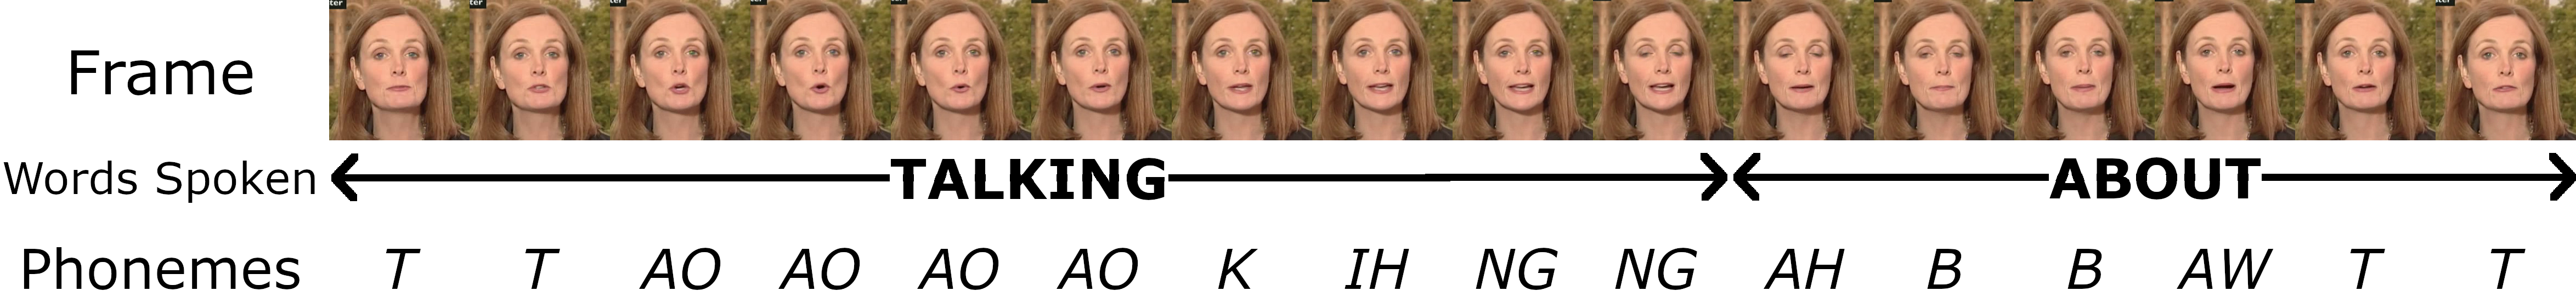
\includegraphics[width=0.9\textwidth]{resources/LRW Example.png}
\caption[A lip reading example from \gls{lrw}.]{A lip reading example from \gls{lrw} \cite{Lip-Reading-In-The-Wild}. This shows the temporal nature of speech, with words spread across frames and being comprised of \gls{phoneme}s. In the example, two words are said: ``TALKING" and ``ABOUT".}
\label{fig:LRW Example}
\end{figure}
\acrfull{ml} is now used for all manner of applications to great success. From stock market prediction to image recognition and even generating artwork, \acrshort{ml} can carry out all manner of complex jobs.\\
Lip reading using \acrshort{ml} is cheap, fast and can be improved over time. \acrshort{ml} models possess the complexity to capture essential nuances within data. Lightweight models can be produced that could run on mobile devices. This makes \acrshort{ml} perfect for the role of lip reading. Lip reading is also largely temporal in nature, as shown in Figure~\ref{fig:LRW Example}, a property that \acrshort{ml} greatly suits. The only downside of \acrshort{ml} is the vast amount of data required, countered only by the abundance of lip reading data and ease of collecting more. In the modern day, there are millions of videos of people speaking, available in just a few clicks online. The average person utters over a hundred words per minute making it easy to collect new data if necessary.\\
The purpose of this paper is to train numerous different models, in tandem, to find the best capable of recognising spoken language. We aim to explore and expand upon other findings within this field and create our own lip reading models.\\
Leading model architectures such as \acrfull{bilstm} Neural Networks, \acrfull{lstm} Neural Networks, \acrfull{cnns} and \gls{transformer}s will be investigated and compared. The performance of such architectures is outstanding for various applications such as video classification, translation and text summarisation. This makes them promising candidates for lip reading.\\
However, lip reading is no easy feat. Various factors make it extremely difficult to predict spoken words using only visual features. The rate of speech, homophones, partial visibility, local dialects, the size of the vocabularies and hard-to-distinguish \gls{viseme}s can make lip reading difficult for humans, let alone computers.\\
Context can be used to give models a way to distinguish between different word senses and homophones, however, this has its own difficulties. Dealing with context can lead to large models and complexity when designing model architectures.

\section{Applications}
The applications of lip reading are expansive. Already, there are modern applications, such as HeyGen\footnote{\url{https://www.heygen.com/}}, which do audio and visual multi-language translation, including altering lip movements to seem more realistic. Imagine being in a meeting with someone from across the world, both able to speak in your native languages, whilst \acrshort{ai} handles the translation.\\
Another application is accessibility support. Cochlear implants and hearing aids are employed by those with hearing loss but they are expensive and invasive, possibly requiring surgery. Lip reading technology could be fitted into a pair of glasses to help people with \acrshort{dhl} on the go. What about even combining the two options above? Imagine a pair of contact lenses or headphones akin to Douglas Adams' Babel fish~\cite{The_Hitch_Hiker's_Guide}.\\
Lastly, lip reading could be crucial for mediums that are visual only. The world is filled with outdated, visual-only surveillance cameras. By employing lip reading technology, words spoken by criminals could be reconstructed and used as evidence for law enforcement. Sound in videos can become corrupted and unavailable but with lip reading, important meeting notes could be reconstructed so that information is never lost. Even noise or distance in environments could be circumvented, allowing two people to communicate whilst across a busy hall without a phone call. The applications are numerous and thrilling.

\section{Aims and Objectives}
\label{sec:Aims and Objectives}
The primary aim of this research is to create a set of \acrshort{ml} models capable of lip reading to find the best architectures. To achieve this there will be various objectives:\\
\begin{enumerate}
  \item Find and gain access to annotated datasets that contain videos of participants speaking
  \item Detect people's faces and localise to their lips, giving image crops or lip landmarks
  \item Develop a data pipeline able to generate useful features for training
  \item Produce a set of models able to capture and identify words being spoken using only visual features
  \item Optimise the various models to achieve a high performance
  \item Compare different architectures and lip reading methods including:
    \begin{itemize}
        \item \acrshort{cnn} architecture followed by \acrshort{lstm} units
        \item A bi-directional architecture
        \item Lip reading based on visual features, lip features and both at once
        \item An attention-based and \gls{transformer} architecture
        \item Using \acrshort{ctc} loss to train lip reading
    \end{itemize} 
  \item Develop a basic \acrfull{gui} to assess model performance in real-time
  \item Extend the \acrshort{gui} to allow for model \gls{fine-tuning}
\end{enumerate}

\section{Report Structure}

This report is split into 5 chapters:
\begin{itemize}
  \item Chapter \hyperref[cha:background]{2} gives a thorough treatment of the background knowledge for the subject area, expanding on some of the physical complications and aspects of lip reading It explains the theory behind various \acrfull{ann} architectures used in the later chapters
  \item Chapter \hyperref[cha:design]{3} addresses the design of the various project stages, including Python software tools that were utilised and the experiment design. It explains the structure of the \acrlong{gui}, giving some examples of it in use
  \item Chapter \hyperref[cha:results]{4} evaluates the different models and experiments, analysing the metrics captured and giving interpretations
  \item Chapter \hyperref[cha:conclusion]{5} summarises the work completed and offers some insights on where this work can be taken next
\end{itemize}           %Chapter 1
%   Intro: ~ 7.5%: 1125 words
        % Current: 1197 words
\chapter{Background}
\label{cha:background}
\graphicspath{ {./resources/} }

\section{Lip Reading}
\label{sec: Lip Reading}
% Intro to what it is
Lip reading is a crucial means of communication. It is one of the few mediums of communication available for people who are hard of hearing or deaf, but all people employ lip reading to a degree. The ability to process the shape of the mouth and lips is essential to everyone during speech processing \cite{lip_reading_used_by_everyone}.\\
Lip reading, or speechreading, refers to being able to understand what a person is saying by using only the visual movements of the face. It is a multimodal communication method; lip reading requires information including the shape of the lips, movement of the tongue and position of the teeth \cite{lip_reading_multimodal}. Context is also crucial for lip reading, having been shown to have a huge impact on the ability to recognise different words \cite{Effects-of-context-type-on-lipreading}.\\
In communication, there are various methods to break down and categorise spoken language. The most popular would likely be \gls{phoneme}s: the fundamental and distinct sounds that are made during speech.
\Gls{viseme}s are another fundamental unit of language. \Gls{viseme}s represent the visual counterparts to \gls{phoneme}s. They are the speech sounds that form similar lip shapes and are thus paramount for lip reading.\\ 
\begin{figure}
\centering
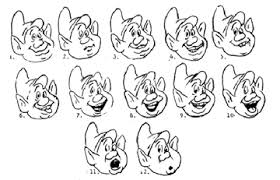
\includegraphics[width=0.5\textwidth]{disney_visemes.jpg}
\caption[The twelve classic Disney \gls{viseme}s.]{The twelve classic Disney \gls{viseme}s. These show the different lip shapes, used by Disney for the 1937 film, Snow White and the Seven Dwarfs, to express different voice noises. Image source: \url{https://docs.cryengine.com/display/SDKDOC2/Phonemes+and+Visemes}}
\label{fig:disney visemes}
\end{figure}
\begin{figure}
\centering
\includegraphics[width=0.5\textwidth]{other_visemes.png}
\caption[OneClick's DAZ Gen8.1 \gls{viseme} example]{OneClick's DAZ Gen8.1. viseme example. These show a more modern, three-dimensional representation of the different \gls{viseme}s used for animation. Image source: \url{https://crazyminnowstudio.com/docs/salsa-lip-sync/modules/recommendations/}}
\label{fig:other visemes}
\end{figure}
However, here is our first problem with lip reading: we do not have a set of consistent \gls{viseme}s. This is primarily an issue highlighted within the domain of animation; animators have to create realistic facial expressions depending on the words being spoken. In the early days of animation, animators realised that different \gls{phoneme}s shared the same facial expression and, therefore, reduced the number of different faces they had to animate. One of the most notable \gls{viseme} sets was Disney's, as shown in Figure~\ref{fig:disney visemes}, which categorises mouth positions into just twelve parts. There are typically ten to fourteen different \gls{viseme}s but there is no global \gls{viseme} set. As shown in Figure~\ref{fig:other visemes}, different animators had different sets of \gls{viseme}s.\\
\begin{figure}
\centering
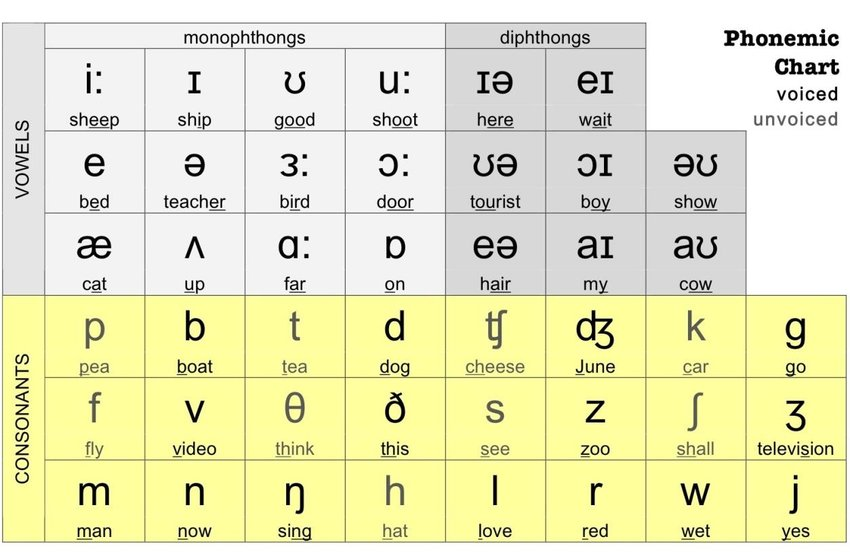
\includegraphics[width=0.5\textwidth]{phoneme_table.png}
\caption[The 44 \Gls{phoneme}s of the English Language.]{The 44 \Gls{phoneme}s of the English Language \cite{44_phonemes}. This represents the widely accepted set of English \gls{phoneme}s, as first presented by Underhil in 2008.}
\label{fig:phoneme table}
\end{figure}
There is another glaring issue with \gls{viseme}s and so lip reading, one that is similar to the everyday homophone. The various \gls{viseme} sets almost always have fewer categories than \gls{phoneme}s do. The consensus in English is that there are 44 unique phonetic sounds, presented in Figure~\ref{fig:phoneme table}. This number is far larger than any set of \gls{viseme}s, which highlights the second major issue with lip reading: the correspondence between \gls{phoneme}s and \gls{viseme}s is tenuous. This is because of visual homophones or homophenes: words that when spoken have different audio components but the same visual components. One of the most famous, and humorous, examples of this is the phrase ``I love you" and ``elephant juice". When spoken aloud these phrases are as different as can be but, for a lip reader, context is needed to tell them apart. Therefore, lip reading is made more complex by the difficult synchronisation between what is spoken and what is visualised.\\
Some studies, such as Bear's ``Which \gls{phoneme}-to-\gls{viseme} maps best improve visual-only computer lip-reading?", have examined which \gls{viseme} sets best map to the \gls{phoneme}s \cite{phoneme_viseme_mapping_review}. However, this study only analyses English \gls{phoneme}s and \gls{viseme}s. As of the time of conducting this research there are 7000 languages spoken worldwide \cite{7000_languages_globally} which might require their own set of \gls{phoneme}s and \gls{viseme}s. There do exist metaphonemes, which are cross-language \gls{phoneme}s \cite{Cross-Linguistic-Phoneme-Correspondences}. However, this would require further analysis into the mapping between these and \gls{viseme}s.\\
Lip reading suffers from all of the difficulties present within classical \acrlong{nlp}, such as homophones, the context being lost, variation in language and ambiguity.\\
Overall, lip reading is an immensely challenging task, one which many fluent speakers can struggle with. From a lack of understanding surrounding \gls{viseme}s, to the thousands of languages spoken around the world, lip reading is hard for people, let alone computers.
\section{Technologies}
This section will delve into the different technologies involved in this research. Various decisions were made surrounding the different tools to employ for data generation, producing a working lip reading model and designing a GUI to showcase the lip reading model.
\subsection{Keras, TensorFlow and PyTorch}
To train \acrshort{ml} models there are two primary libraries: TensorFlow\footnote{\url{https://www.tensorflow.org/}} and PyTorch\footnote{\url{https://pytorch.org/}}. These provide various functionality, such as being able to define \acrlong{anns}, perform mathematical operations on batched data and format sparse or big data. It is important to note that TensorFlow contains another API called Keras\footnote{\url{https://keras.io/}}.\\
There is wide discourse as to which tool is the best. PyTorch is low level, high-performance, easier to debug but less readable. TensorFlow is high and low-level, high-performance, has better readability but is harder to debug. Keras is the most popular of all three. Whilst PyTorch is written in Lua and TensorFlow in a combination of C\texttt{++}, CUDA and Python, Keras is only written in Python. Keras has lower performance but makes up for this with its simplicity and code readability \cite{Keras-vs-TF-vs-PT}. Typically, TensorFlow is regarded as being used more in industry whilst PyTorch is used primarily for research.\\
I decided to go with the popular consensus and use Keras. Its simplicity and readability would be advantageous since I have not made use of any of these tools before. Furthermore, as I am more experienced in Python, this would better suit my skill set. Although it is lower performance than the other libraries, I will only be creating relatively small models and have access to quite powerful \acrshort{gpu}s for training. Furthermore, this research may be useful to get more experience in the industry standard libraries employed for \acrshort{ml}.
\subsection{MediaPipe and Dlib}
\label{sec:mediapipe}
\begin{figure}
\centering
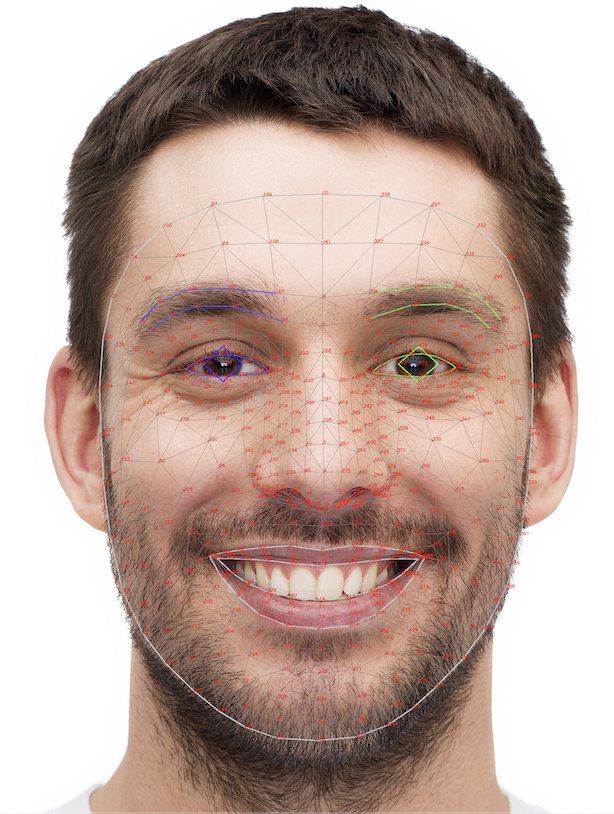
\includegraphics[width=0.5\textwidth]{mediapip_landmarks.png}
\caption[Visualizing the 478 MediaPipe facial landmark coordinates.]{Visualizing the 478 MediaPipe facial landmark coordinates. This image gives a map of the different MediaPipe facial landmarks, labelling each with its index. Image source: \url{https://developers.google.com/mediapipe/solutions/vision/face_landmarker}}
\label{fig:mediapipe landmarks}
\end{figure}
MediaPipe\footnote{\url{https://developers.google.com/mediapipe}}  is an innovative Machine Learning framework developed by Google. MediaPipe provides various functionalities such as gesture tracking, object classification, audio processing and natural language processing. The framework allows for efficient resource management, allowing both GPU and CPU utilisation to increase the performance of running \acrshort{ml} models \cite{mediapipe_info}. Shown in Figure~\ref{fig:mediapipe landmarks}, one notable tool is MediaPipe's Face Landmark Detection\footnote{\url{https://mediapipe-studio.webapps.google.com/demo/face_landmarker}}. This provides a library for detecting faces within images and estimating hundreds of facial landmarks such as the lips, eyes and nose. \\
\begin{figure}
\centering
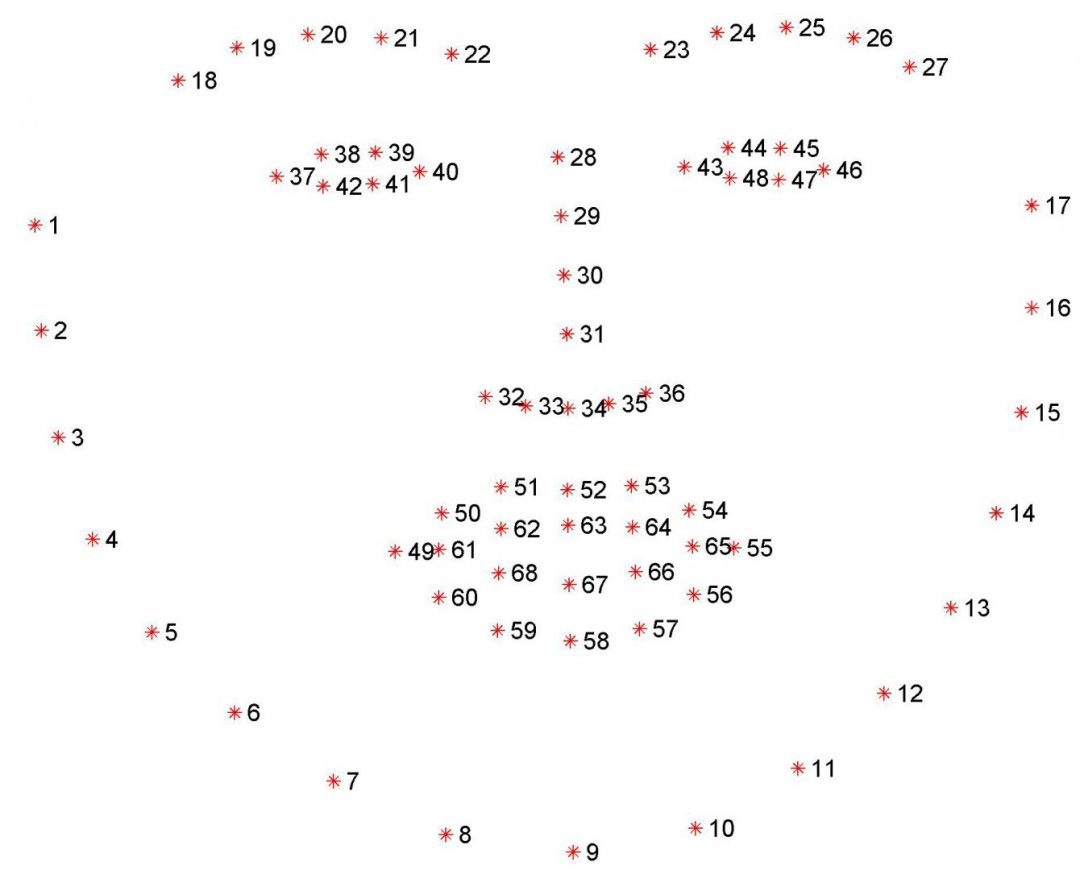
\includegraphics[width=0.5\textwidth]{dlib_landmarks.jpg}
\caption[Visualizing the sixty-eight Dlib facial landmark coordinates.]{Visualizing the sixty-eight Dlib facial landmark coordinates. This gives a map of Dlib's facial landmarks, giving the index of each different landmark. Image source: \url{https://pyimagesearch.com/2017/04/03/facial-landmarks-dlib-opencv-python/}}
\label{fig:dlib landmarks}
\end{figure}
Dlib is a C++ toolkit that contains a diverse selection of Machine Learning solutions. Dlib is primarily a collection of various software components \cite{dlib_info}, the most notable being its Face Detector\footnote{\url{http://dlib.net/face_detector.py.html}}, shown in Figure~\ref{fig:dlib landmarks}. This class can detect faces within images and return the coordinates of facial landmarks.\\
Another major technological decision was whether to utilise MediaPipe or Dlib for collecting data to train the lip reading models. A crucial step for this research is being able to localise to a person's lips to collect data for inference, much like a person does in conversation.\\
In total MediaPipe detects 478 3D facial landmarks, forty of which are directly associated with the lips. Dlib detects sixty-eight 2D facial landmarks, nineteen of which are related to the lips. Further investigation could be done into which performs the best at localising to faces but this difference will likely be insignificant. The more important difference between these two libraries is their landmark data.\\
A major part of \acrshort{ml} is \gls{feature_extraction}. Facial landmarks extracted from images could be useful to train an \acrshort{ann} to focus directly on the shape of the lips when different \gls{phoneme}s are being said. These could significantly cut down on noise within data, using transfer learning to make a more accurate model.\\
Consequently, the clear choice is to use MediaPipe. It provides more information associated with the lips: there are more than double the landmarks, all of which are a higher dimension than the landmarks generated by Dlib.
\subsection{Tkinter}
Tkinter\footnote{\url{https://docs.python.org/3/library/tkinter.html}} is a Python package that interfaces the Tk \acrfull{gui} toolkit. It is a package for producing various cross-platform GUI applications with a native look and feel \cite{An-introduction-to-tkinter}.\\
There is much discussion about which Python GUI package to use, some popular choices include PySimpleGUI\footnote{\url{https://www.pysimplegui.org/en/latest/}}, Flexx\footnote{\url{https://flexx.readthedocs.io/en/stable/}} and Ipywidgets\footnote{\url{https://ipywidgets.readthedocs.io/en/stable/}}.\\
For this project, Tkinter will be used due to its simplicity, ability to be run on different Operating Systems and its accessibility (Tkinter is pre-installed on Python) \cite{comparing_python_guis}. Tkinter has good flexibility and I have experience with this tool already. Therefore, the focus of the project will remain on lip reading rather than learning a new Python \acrshort{gui} tool.
\subsection{NLTK}
\label{sec: nltk}
% For getting phonemes
% Reference here how we get visemes
NLTK\footnote{\url{https://www.nltk.org/}} is a Python library for \acrlong{nlp} and text analytics \cite{nltk_info}. It provides various tools for processing text like lemmatisation, tagging, tokenisation and word normalisation. Moreover, NLTK contains numerous \gls{corpora}.\\
One useful tool provided by NLTK is the Carnegie Mellon Pronouncing Dictionary (cmudict)\footnote{\url{https://www.nltk.org/_modules/nltk/corpus/reader/cmudict.html}}. This reduces English words to their constituent \gls{phoneme}s.\\
As there is no standard set of \gls{viseme}s, NLTK cannot be used as a \acrfull{p2v} mapper: a tool that would be crucial for generating \gls{viseme} data. Research suggests \cite{phoneme_viseme_mapping_review} that the best correspondence between \gls{phoneme}s and \gls{viseme}s is Lee \cite{best_phoneme_viseme_mapping}. This maps \gls{phoneme}s to six consonant \gls{viseme}s and seven vowels \gls{viseme}s. It also has a silence \gls{viseme} \cite{best_phoneme_viseme_mapping}. This \acrshort{p2v} map will be hardcoded into a dictionary to easily convert from \gls{phoneme}s to \gls{viseme}s. So, NLTK could be used to convert words to their constituent \gls{phoneme}s before this \acrshort{p2v} mapping is used to convert again to \gls{viseme}s.
\subsection{JiWER}
\label{sec: JiWER}
JiWER\footnote{\url{https://pypi.org/project/jiwer/}} is a Python library that supports various \acrfull{asr} tasks. JiWER has been used to compare the performance of various \acrshort{asr} systems \cite{jiwer_example}. It provides various useful functions such as calculating the \acrfull{wer} and \acrfull{cer}, intrinsic for comparing lip reading model performance.\\
The \acrshort{wer} is defined as 
\[WER = \frac{S_w + D_w + I_w}{H_w + S_w + D_w} = \frac{S_w + D_w + I_w}{N_w},\]
where $WER$ is the word error rate, $S_w$ the number of substitutions (in the predicted phrase), $D_w$ the number of deletions, $I_w$ the number of insertions, $H_w$ the number of correct words (or hits in the predicted phrase) and $N_w$ is the number of words (in the reference phrase) \cite{jiwer_example}.\\
The \acrshort{cer} is defined similarly, although rather than looking at words it focuses on individual letters
\[CER = \frac{S_c + D_c + I_c}{H_c + S_c + D_c} = \frac{S_c + D_c + I_c}{N_c}.\]
In these equations, the subscript $w$ signifies variables at the word level and subscript $c$ at the character level.
\section{Artificial Neural Networks}
An \acrfull{ann} is a structure inspired by the brain. It is a set of connected artificial nodes, like mathematical functions, that take input from previous nodes and pass this to later nodes.\\
This section will cover various fundamental concepts for \acrshort{ml} and training an \acrshort{ann}.
\subsection{Softmax}
\begin{figure}
\centering
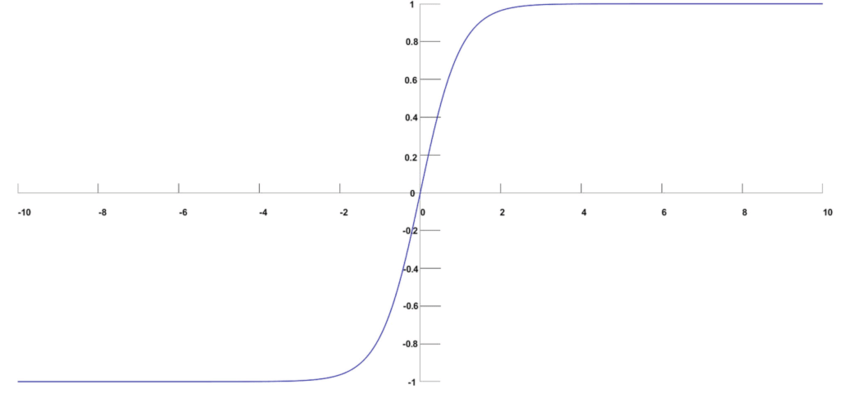
\includegraphics[width=0.7\textwidth]{Softmax-function-image.png}
\caption[Softmax function image.]{Softmax function image \cite{softmax_diagram}.}
\label{fig:softmax}
\end{figure}
Softmax is a crucial but easy mathematical function, shown in Figure~\ref{fig:softmax}, often used as the final \gls{activation_function} within \acrshort{anns}. Softmax is used to normalise a set of numbers so that they sum to 1 \cite{softmax}. Consequently, it is often used to normalise the output of an \acrshort{ann} to give the probability that data samples belong to each class within a set.\\
The Softmax, $\sigma(x)_i$, for each element $x_i$ of a vector is defined as
\[\sigma(\mathbf{x})_i = \frac{e^{x_i}}{\sum^{K}_{j=1}e^{x_j}},\]\\
where there are $K$ classes, $i, j = 1,2,...K$ and $\mathbf{x} = (x_1, x_2,...x_K)$.
\subsection{ReLU}
\label{sec: relu}
\begin{figure}
\centering
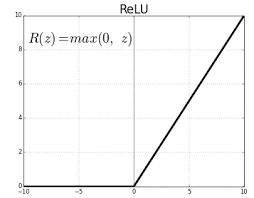
\includegraphics[width=0.5\textwidth]{ReLU Diagram.png}
\caption[Graph of ReLu \gls{activation_function}.]{Graph of ReLu \gls{activation_function}~\cite{relu_diagram}.}
\label{fig:ReLU}
\end{figure}
To train an \acrshort{ann}, the outputs of each layer are passed through a nonlinear function: an \gls{activation_function}. Shown in Figure~\ref{fig:ReLU}, ReLU is a commonly used, simple and efficient \gls{activation_function} within \acrshort{ml} \cite{relu_description}.\\
\acrshort{anns} trained using ReLU typically perform better than those trained using other \gls{activation_function}s, such as the tanh function \cite{relu_is_the_best}.\\
ReLU, $R$, will output the input, $z$ if it is positive but otherwise give the value 0.
\subsection{Cross-Entropy Loss}
\label{sec: Cross-Entropy Loss}
Loss is a crucial measurement within \acrshort{ml}. Loss measures the difference between the predicted and the true classes of data samples. Most methods for training an \acrshort{ann}, such as \acrfull{sgd}, aim at reducing loss for a set of data samples. But, depending on the task, there are many different loss measurements.\\
Cross-entropy loss is employed during training of \acrshort{ann}s that output the probability that a given data sample belongs to a class. Cross-entropy measures the difference between the true probability and a model's predicted probability. A value of 0 means that the model perfectly predicts the probability \cite{cross_entropy_loss}.\\
There are different flavours of cross-entropy, depending on the task. For example, binary cross-entropy is used when there are only two different classes of data. Categorical cross-entropy is used for \gls{multi-class}.\\
In \gls{multi-class}, an \acrshort{ann} will output the probability that a data sample belongs to each different class. Therefore, categorical cross-entropy is employed to increase this probability for the correct class of a sample and reduce the probability for incorrect classes.\\
Categorical cross-entropy will be employed during training of lip reading models as this is a \gls{multi-class} problem; we have a video containing one of $X$ words (or \gls{phoneme}s, or \gls{viseme}s).\\
The formulation for cross-entropy loss, $L$, over $N$ classes is defined as\\
\[L = - \sum_{i=1}^{N} y_i \log{p_i},\]\\
where $y_i$ is the truth value, of whether a data sample is in class $i$, and $p_i$ is the Softmax probability for the class $i$. For training, there are four classes so this can be expanded further:\\
\[L = - [ y_0 \log{p_0} + y_1 \log{p_1} + y_2 \log{p_2} + y_3 \log{p_3}].\]
\subsection{Long-Short Term Memory}
A \acrlong{rnn} is a type of \acrshort{ann} used in \acrfull{dl} for sequential data such as text, audio and videos. There are different types of \acrshort{rnn} classified by their structure, such as classic \acrshort{rnn}, \acrshort{lstm}, \acrshort{gru}, Attention \acrshort{rnn} and \gls{transformer}s. The choice of \acrshort{rnn} unit largely depends on the task being carried out, for example the \gls{transformer} architecture is primarily used for modern large language models such as  ChatGPT\footnote{\url{https://chat.openai.com/}}.\\
\begin{figure}
\centering
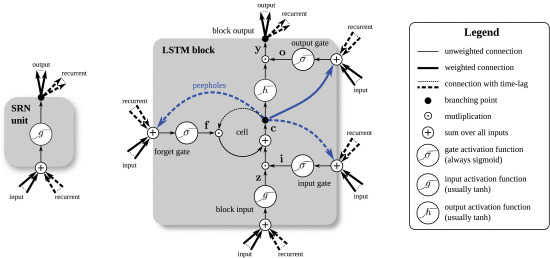
\includegraphics[width=0.9\textwidth]{lstm_diagram.jpg}
\caption[Detailed diagrams of a \acrfull{sru} and \acrfull{lstm} Unit.]{Detailed diagrams of a \acrfull{sru} and \acrfull{lstm} \cite{lstm_diagram}. A \acrshort{sru} is shown on the left and an \acrshort{lstm} block on the right as used in the hidden layers of a recurrent neural network.}
\label{fig:lstm diagram}
\end{figure}
\acrfull{lstm} is an \acrshort{rnn} cell operation first proposed to overcome the vanishing gradient problem \cite{OG_LSTM}. \acrshort{lstm} overcame many of the shortcomings of early, vanilla \acrshort{rnn}s and allowed for both short and longer term dependencies to be established within sequential data.\\
\begin{figure}
\centering
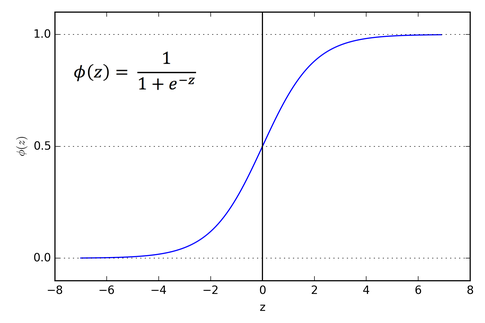
\includegraphics[width=0.5\textwidth]{Sigmoid Activation Function.png}
\caption[Graph of the Sigmoid Activation function.]{Graph of the Sigmoid Activation function. Image source:\\ \url{https://towardsdatascience.com/activation-functions-neural-networks-1cbd9f8d91d6}.}
\label{fig:sigmoid diagram}
\end{figure}
\acrshort{lstm} is comprised of three gates called the input, output and forget gates. Shown in Figure~\ref{fig:lstm diagram}, these gates give \acrshort{lstm}s the ability to alter or drop data from a sequence \cite{Deep-learning:-RNNs-and-LSTM}. This makes them useful for processing video data where there are long-term dependencies between frames and speech containing \gls{speech_disfluency} or features that need to be ignored. The gates are computed using sigmoid \gls{activation_function}s, shown in Figure~\ref{fig:sigmoid diagram}. LSTM has also been shown to be successful for video facial recognition tasks in the past \cite{facial_expression_rec_lstm}.\\
\begin{figure}
\centering
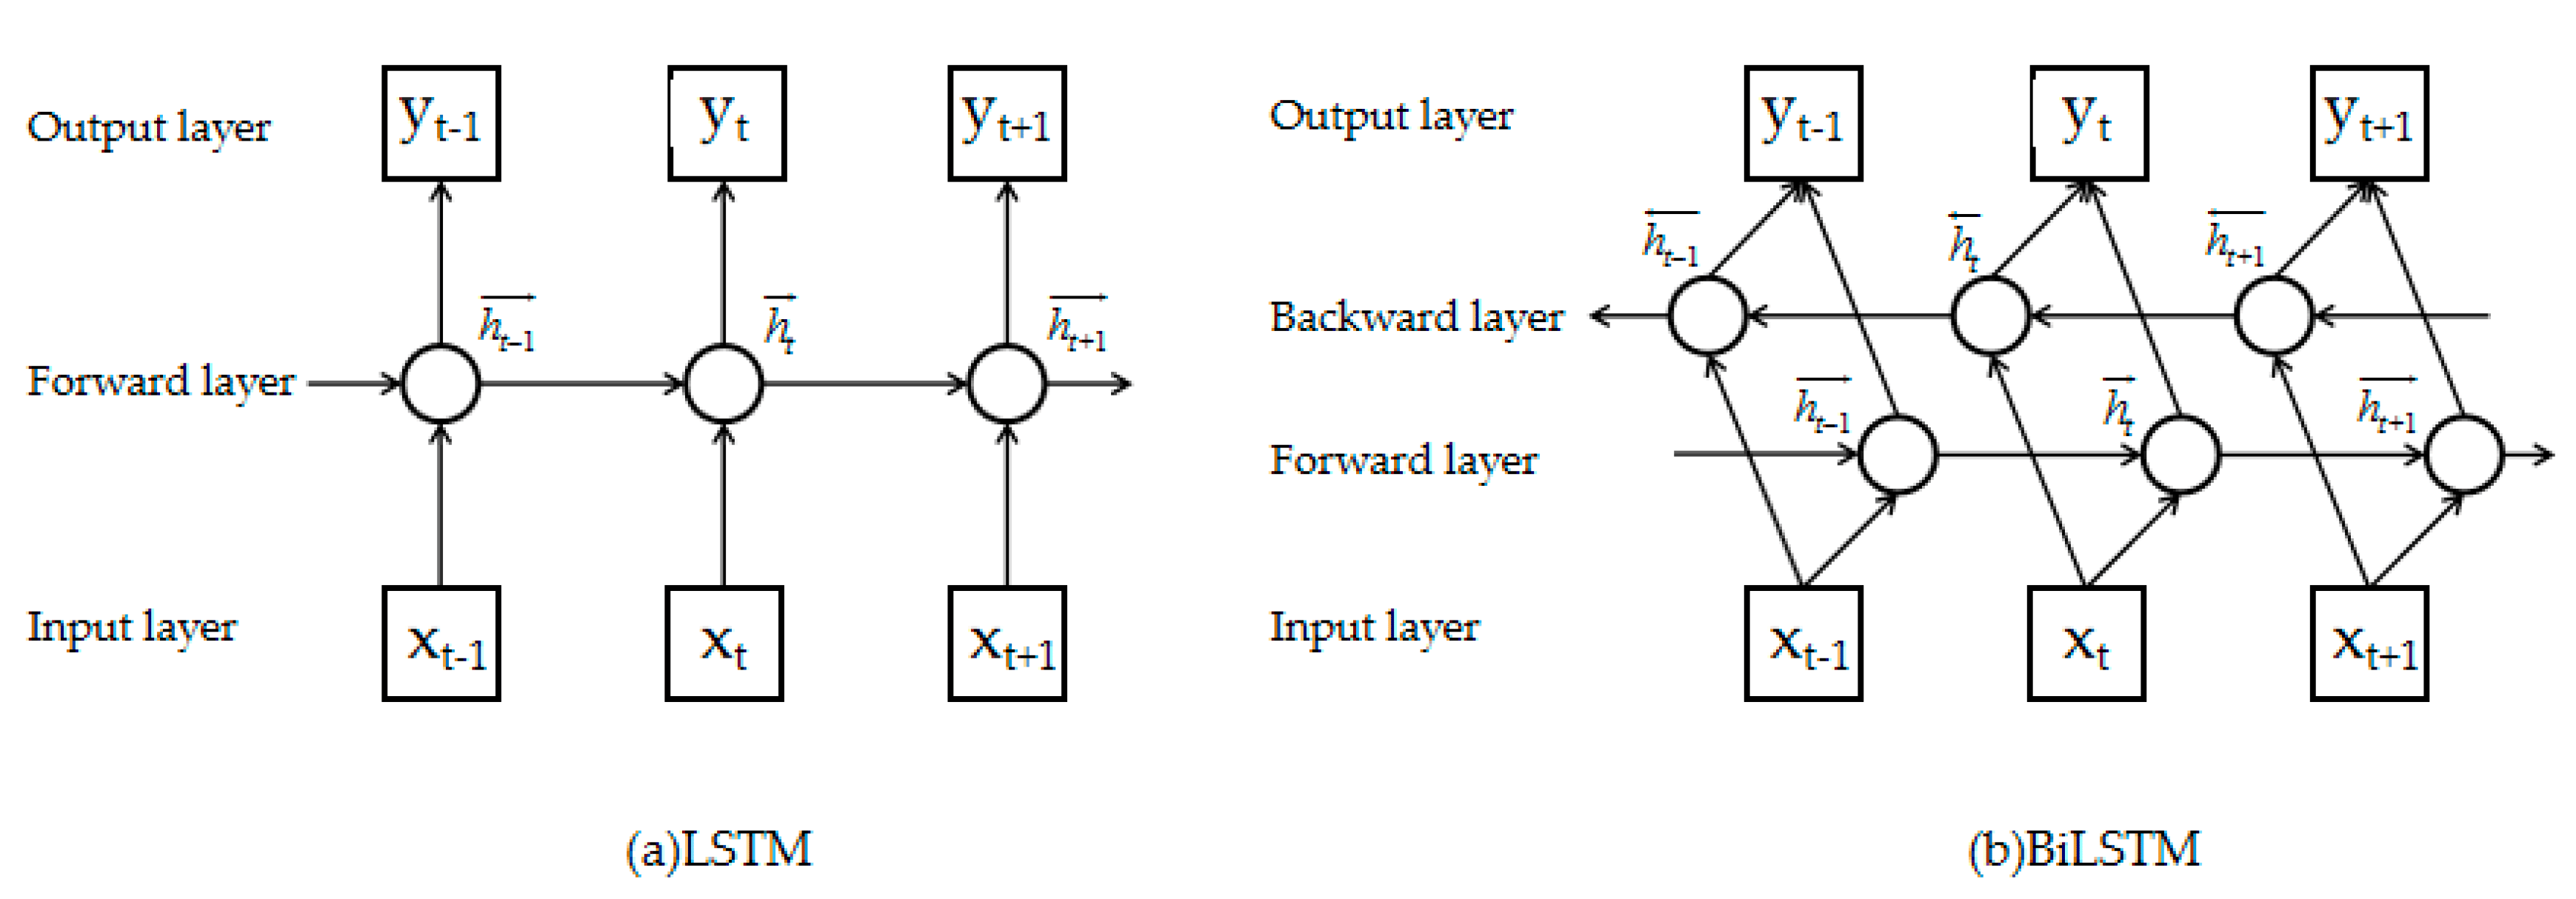
\includegraphics[width=0.7\textwidth]{bilstm.png}
\caption[The architecture of the (a) LSTM model and (b) BiLSTM model.]{The architecture of the (a) LSTM model and (b) BiLSTM model~\cite{bilstm_diagram}.}
\label{fig:bilstm diagram}
\end{figure}
A notable extension to typical \acrshort{rnn}s is that of a bidirectional \acrshort{rnn}. This allows consideration of both left and right context: events that happened in both the past and future. Bidirectional \acrshort{rnn}s have been used to derive \acrfull{bilstm} (shown in Figure~\ref{fig:bilstm diagram}) and \acrfull{bigru}. However, the main downside of these networks is that they require training two separate architectures simultaneously.
\subsection{Convolutional Neural Networks}
\begin{figure}
\centering
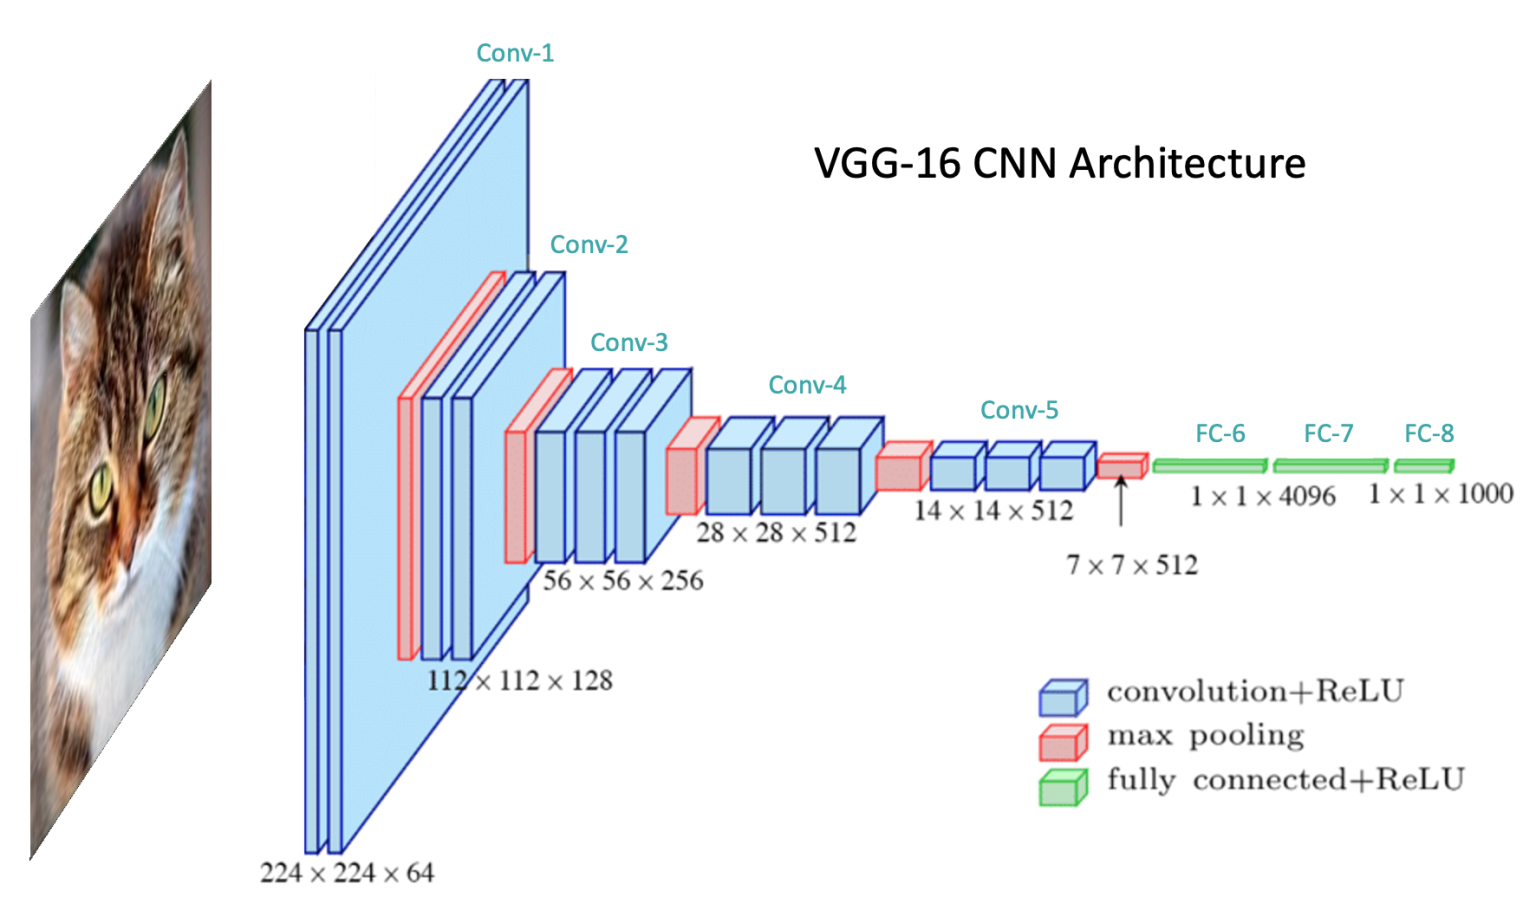
\includegraphics[width=0.7\textwidth]{CNN Diagram.png}
\caption[The VGG-16 \acrfull{cnn} Architecture.]{The VGG-16 \acrfull{cnn} Architecture~\cite{vgg_architecture}. This depicts the main features of a \acrshort{cnn}: convolutional layers, max pooling layers and a final set of fully-connected layers. Image source: \url{https://learnopencv.com/understanding-convolutional-neural-networks-cnn/}}
\label{fig:cnn diagram}
\end{figure}
Primarily used to solve image classification tasks, \acrfull{cnns} are a powerful \acrshort{ann} architecture \cite{cnn_intro, Convolutional-neural-network:-a-review-of...}. \acrshort{cnn}s are characterised by three primary components: convolutional layers, max pooling layers and a final set of fully-connected layers \cite{cnn_intro}.\\
The operation of convolutional layers hinges on filters (also called kernels), comprised of trainable parameters, that are convolved across an image \cite{Convolutional-neural-network-(CNN)-for-image-detection-and-recognition, Convolutional-neural-network:-a-review-of...}. Convolution can be done on images if the layer is the first within the network, like \emph{Conv-1} in Figure~\ref{fig:cnn diagram}, or otherwise the output from the previous layer, called a hidden representation.\\
Convolution functions by the filter being slid across the input array. The scalar product between the filter and the current image region is calculated and placed at the centre point of the filter within the image.\\
The output, $C$, of a convolutional layer at the position $(a,b)$ is thus given as
\[C_{a,b} = \sum^{f-1}_{i=0}\sum^{f-1}_{j=0}w_{i,j} \cdot X_{i+a,j+b},\]\\
where $X$ is the input, of size $N\times N$, and $w$ is the filter, of size $f\times f$.\\
Presented here is 2D convolution, however, there also exists 1D and 3D convolutional layers, the difference being the filter and data size. 3D convolution is typically used for video data and requires 3D matrices of filters.\\ 
Max pooling layers are simpler, instead being used to reduce the size of a hidden representation within a model \cite{cnn_intro}. Max pooling layers similarly convolve across the output of the previous \acrshort{ann} layer, taking the maximum value in each pooling region to be the output, thus capturing the strongest activations \cite{max_pooling_&_dropout}. This effectively reduces the effect of noise and reduces the size of data whilst remaining computationally efficient.\\
The output of a max pooling layer, $M$, at the position $(i,j)$ and the size of the output, $m$, are defined as
\[M_{i,j} = max(X_{i-(f/2),j-(f/2)},...X_{i+(f/2),j+(f/2)}),\]
\[m = \frac{N - f}{s} + 1,\]
where $s$ is the stride size: how many positions the filter is moved in each operation \cite{Pooling-methods-in-deep-neural-networks}.\\
A fully-connected layer is classified by its neurons. Every neuron of a fully-connected layer is connected to every single neuron from the previous layer \cite{cnn_intro}.\\
Overall, \acrshort{cnn}s are fantastic to better visualise and identify possible problems models may have with the underlying data thus forming useful, general models to be used for \gls{feature_extraction} or otherwise \cite{Visualizing-and-understanding-convolutional-networks}. \acrshort{cnn}s have proven themselves time and time again as excellent architectures for visual-based models.
\subsection{Attention}
\label{sec: Attention}
Attention is a modern and popular method for speech recognition and language-based problems \cite{Effective-Approaches-to-Attention-based-Neural-Machine-Translation}. It offers fantastic performance for machine translation and is capable of understanding longer utterances than those present within the training data \cite{Attention-based-models-for-speech-recognition}. Some similar work, with attention for lip reading, has even used this to great success in the past \cite{lipreading_with_attention}.\\
Attention mimics how humans form information: by selectively building connections between different parts of information, rather than considering the entire context at once \cite{A-review-on-the-attention-mechanism}. The major benefit of this, for lip reading, is that it allows for ignoring \gls{speech_disfluency}, mapping varying numbers of states within the input sequence to the output sequence and focusing on crucial details within a sequence.\\
To calculate attention, there are three main components: the key ($K$), the query ($Q$), and the value ($V$). $K$ encodes the source data feature, $Q$ is a task-related representation (often the output we want to get) and $V$ is a new data feature representation \cite{A-review-on-the-attention-mechanism}. $V$ is usually an alternate representation of the original sequence or even just the same as $K$ \cite{A-review-on-the-attention-mechanism}.\\ 
Here the standard, scaled dot-product attention will be used, rather than the other forms of attention. This is the default offered by the Keras library\footnote{\url{https://keras.io/api/layers/attention_layers/attention/}}. This is defined as
\[Attention(Q, K, V) = softmax(\frac{QK^{T}}{\sqrt{|K|}}) \cdot V,\]\\
where $Q$ is the query, $K$ is the key and $V$ is the value.\\
Self attention is defined as attention where $Q$, $K$ and $V$ are all the same sequence. This method offers the advantage of self-alignment, enabling the identification of the importance of particular states within a sequence in relation to other states \cite{self_attention}.
\subsection{Stochastic Gradient Descent}
\begin{figure}
\centering
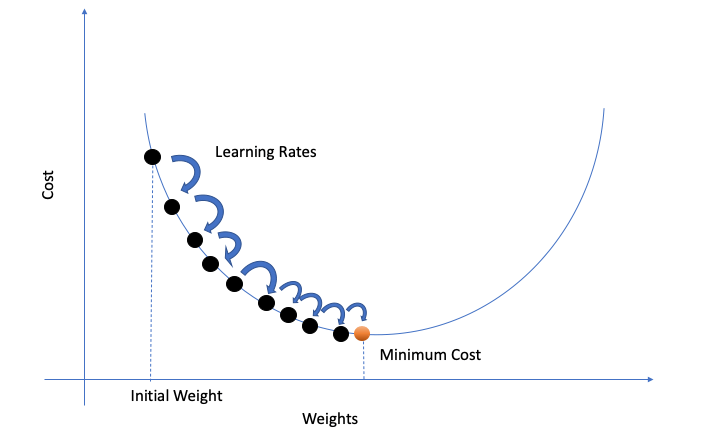
\includegraphics[width=0.7\textwidth]{Stochastic-Gradient-Descent.png}
\caption[Stochastic Gradient Descent.]{Stochastic Gradient Descent~\cite{sgd_diagram}. Here we can see how cost, or loss, is reduced via Stochastic Gradient Descent. This is the ideal for training, where we want to optimise our weights to achieve as small a loss as possible and so an optimal model.}
\label{fig:Stochastic Gradient Descent}
\end{figure}
Training an \acrshort{ann} is an iterative optimisation problem, where the goal is to find the inputs that minimise the output of an objective function \cite{Stochastic-gradient-descent}. At present, gradient descent is the most popular method for solving such a problem. Gradient descent, represented in Figure~\ref{fig:Stochastic Gradient Descent}, uses the first-order derivative to make small, iterative steps in the opposite direction to the gradient of the loss function. This leads to the minima and the most optimal \acrshort{ann} weights for a given problem.\\
Stochastic mini-batch gradient descent is a variation of this process, where each update utilises a random subset of data samples to adjust the network weights \cite{Stochastic-gradient-descent}. This is opposed to just using a single data sample or the entire dataset (stochastic and batch gradient descent, respectively). Mini-batch gradient descent boasts several advantages over other methods, such as reduced computational cost, reduced noise and \gls{overfitting} avoidance \cite{Stochastic-gradient-descent}.\\
Two parameters crucial to \acrshort{sgd} are \acrlong{lr} and batch size.\\
\subsubsection{Learning Rate}
\begin{figure}
\centering
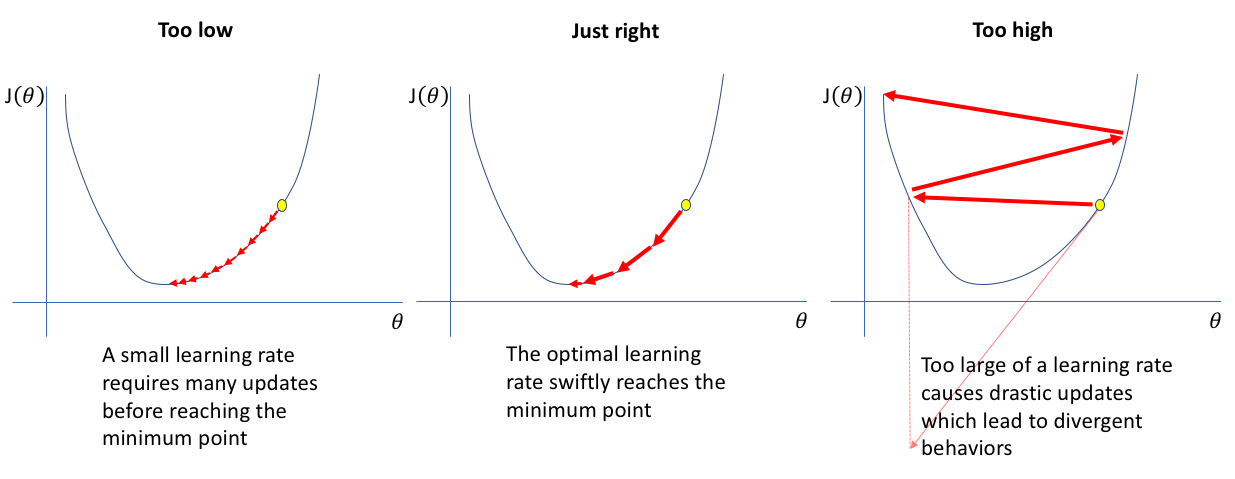
\includegraphics[width=0.7\textwidth]{Learning Rate.png}
\caption[The effects of varying \acrshort{lr}.]{The effects varying \acrshort{lr}. This shows how too high or low \acrshort{lr} can cause problems when minimising a loss function. Image source: \url{https://www.jeremyjordan.me/nn-learning-rate/}.}
\label{fig:Learning Rate}
\end{figure}
\acrfull{lr} relates to the size of steps within \acrshort{sgd}. Finding the optimal \acrshort{lr} is a difficult task requiring tuning \cite{adadelta_adaptive_learning_rate}. As show in Figure~\ref{fig:Learning Rate}, electing too high an \acrshort{lr} could prevent any minima ever being found, whilst too low could slow training significantly and find local minima \cite{adadelta_adaptive_learning_rate}. \acrshort{lr} is one of the leading causes of \gls{overfitting} within \acrshort{ml}, so is a crucial design decision \cite{learning_rate_causes_overfitting}.\\
\begin{figure}
\centering
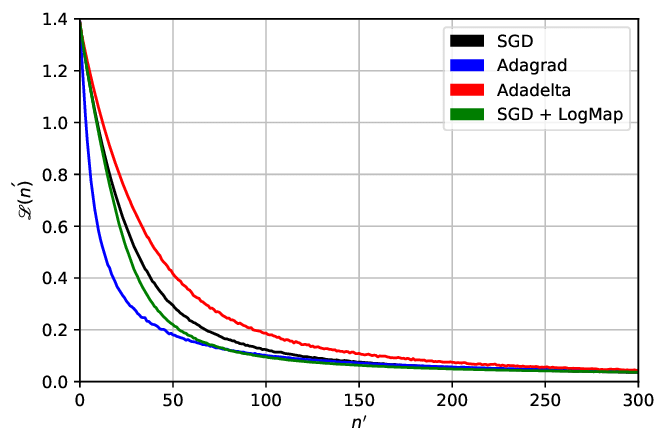
\includegraphics[width=0.7\textwidth]{Adaptive Learning Rate.png}
\caption[The advantage of Adagrad with the adaptive \acrshort{lr} over other \acrshort{lr} methods.]{The advantage of Adagrad with the adaptive \acrshort{lr} over other \acrshort{lr} methods~\cite{adaptive_learning_rate_diagram}. This shows the impact of utilising Adagrad, an adaptive \acrshort{lr} scheduler over regular \acrshort{sgd}. Here the same loss was achieved in far fewer epochs. The choice of \acrshort{lr} scheduler is crucial as it could produce worse results, such as with Adadelta.}
\label{fig:Adaptive Learning Rate}
\end{figure}
Recently multiple methods have been developed to vary \acrshort{lr} over time, rather than keeping it static throughout training \cite{Learning-an-adaptive-learning-rate-schedule}. Some of the different dynamic \acrshort{lr}s are shown in Figure~\ref{fig:Adaptive Learning Rate}. Adaptive \acrshort{lr} can save computational time whilst still finding the global minimum: the best of both stochastic and batch gradient descent.\\
The choice of \acrshort{lr} scheduler, or optimiser, is incredibly important, possibly increasing or decreasing the number of epochs required for training. Some examples include linear decay, Adadelta, Adam and exponential decay \cite{Learning-an-adaptive-learning-rate-schedule}.\\
\subsubsection{Batch Size}
\label{sec: Batch Size}
Batch size is the number of samples used within one training pass of a neural network \cite{batch-size-on-the-generalizability}. Difficult to tune, batch size dramatically impacts the performance of neural networks.\\
Various research has been done into the impact of batch size, concluding that, for image classification, a higher batch size produces better performance \cite{batch-size-on-the-performance}. However, this is not always the case. The option of batch size depends on the task being carried out and the other hyperparameters within the experiment \cite{batch-size-on-the-generalizability}. With a large \acrshort{lr} it is better to use a large batch size, and for a small \acrshort{lr}, a small batch size is better \cite{batch-size-on-the-generalizability}.\\
This is due to the roles of batch size and \acrshort{lr}. With a high \acrshort{lr} we have that the model changes dramatically based on the data but if we have a small batch size and little data, the model may become biased towards just these samples. Models could overfit, becoming too focused on the small dataset given. Alternatively, with a low \acrshort{lr} and high batch size, the model may not learn any new information or change very much.\\
Another side effect of batch size is computational cost and efficiency. Larger batch sizes necessitate more calculations thus incurring increased computational costs \cite{batch-size-on-the-performance}. However, larger batch sizes can increase computational efficiency attributed to better data and operation parallelism \cite{Adaptive-Batch-Sizes}.\\
To optimise the training process, a high \acrshort{lr} and batch size should be used initially, reducing these values throughout until only finetuning is required \cite{batch-size-on-the-generalizability}. This balances computational cost and model efficiency. Suggested values for the batch size are around 32 samples and, therefore, this will be used within the experiments unless a more suitable size is identified.
\subsection{Connectionist Temporal Classification Loss}
\label{sec: CTC Loss}
\begin{figure}
\centering

\includegraphics[width=0.7\textwidth]{CTC Audio.png}
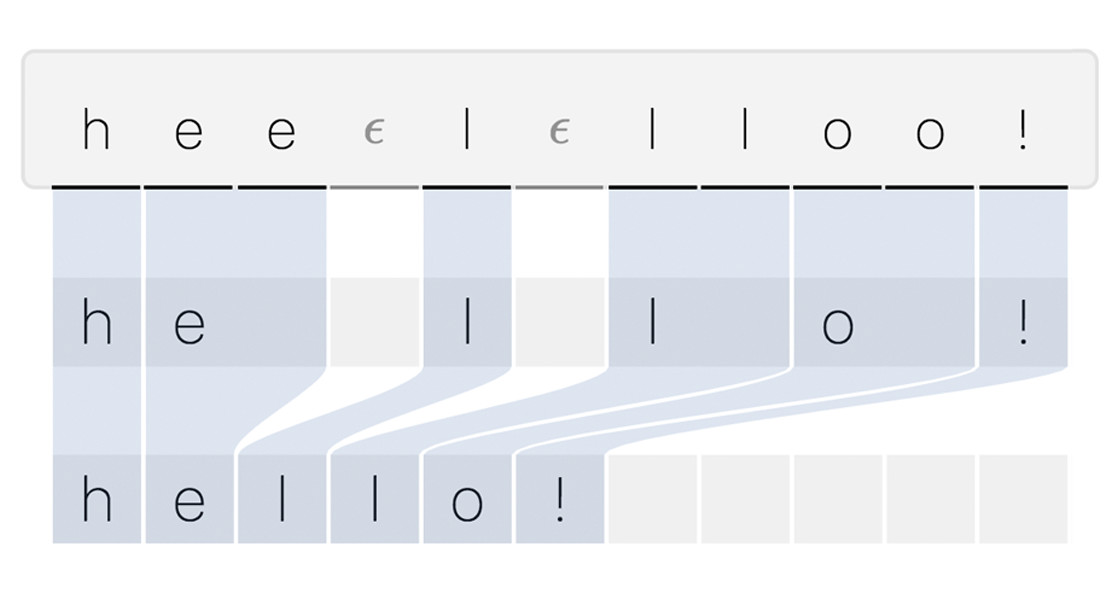
\includegraphics[width=0.7\textwidth]{CTC Loss.jpg}
\caption[\acrshort{ctc} Loss on an audio sequence.]{\acrshort{ctc} Loss on an audio sequence. This shows how CTC loss can be used to predict a sequence of tokens which can then be merged into spoken information. Image source: \url{https://distill.pub/2017/ctc/}.}
\label{fig:CTC Loss}
\end{figure}
\acrfull{ctc} \cite{original_CTC} is a loss metric utilised for sequencing labelling problems where the alignment between the sequence and labels is unknown \cite{exploration-of-CTC-acoustic-models}. The type of alignment found using \acrshort{ctc} loss is depicted within Figure~\ref{fig:CTC Loss}. \acrshort{ctc} loss is used for various speech recognition problems including \acrshort{asr} and lip reading, offering excellent performance \cite{LCANet, LipReading-with-3D-2D-CNN-and-word-CTC-models}.\\
\acrshort{ctc} loss automatically learns connections between sequence frames and labels, removing the need for individual frame labelling \cite{exploration-of-CTC-acoustic-models}. Furthermore, compared with other methods, \acrshort{ctc} loss produces models that are smaller and faster \cite{ctc_faster_models}. Much work has been done within this area and so this method will additionally be incorporated and compared with others for lip reading.\\
For lip reading, \acrshort{ctc} loss will take the form of finding the most likely words (or letters, phonemes or visemes) given the input video feed.\\
First proposed in 2006, \acrshort{ctc} loss aims to find the most likely label sequence, $Y = (y_1, y_2,..., y_U)$ for a given input sequence, $X = (x_1, x_2,...,x_T)$ \cite{original_CTC}. Here, $y(u)$ is the target symbol at time step $u$ and $x(t)$ is the input state at time step $t$. So, we can define the output sequence, $Y^*$ as
\[Y^* = \argmax_Y  P(Y|X)\]\\
This probability is simplified to
\[P(Y|X) = \Sigma_{A \in X, Y} P(A|X)\]
\[P(Y|X) = \Sigma_{A \in X, Y} \prod_{t = 1}^T P_t(a_t|X)\]
\[\therefore Y^* = \argmax_Y \Sigma_{A \in X, Y} \prod_{t = 1}^T P_t(a_t|X)\]\\
Where $A$ represents the alignments from the input to output sequence and $a_t$ the alignment at time step $t$ \cite{original_CTC}.\\
This can then be used to train the model's parameters. By trying to maximise the likelihood of the correct $Y^*$ or minimising the negative log-likelihood  (shown below), we can optimise the model's parameters \cite{original_CTC}.
\[CTC\ Loss = - \Sigma_{(X, Y)} log P(Y|X)\]\\
Training using CTC loss is computationally expensive, as finding the optimal alignments, requires dynamic programming \cite{original_CTC}.
\section{Related Work}
It is important to understand the accomplishments and failures of past work, in the field of automated lip reading, to inform a way forwards.\\
One of the most famous lip reading solutions was proposed by Chung et al.~\cite{Lip-Reading-In-The-Wild} in 2016. Chung et al. generated a huge dataset of word utterances from BBC\footnote{\url{https://www.bbc.co.uk/}} broadcasts, now referred to as \gls{lrw}. This was key to the development of lip reading models and made it possible for others to build upon their work. Their published dataset became widely used due to its easy access and high quality.\\
They proposed a series of different \acrshort{cnn} based architectures for lip reading, which exceeded the public performance benchmark at the time. Furthermore, they speculated about utilising \acrshort{lstm} units to better understand full sentences, rather than just single utterances. This forms a good place to start training.\\
In 2020, Luo et al.~\cite{Synchronous-Bidirectional-Learning-for-Multilingual-Lip-Reading} utilised an encoder and bidirectional decoder architecture to carry out multilingual lip reading by classifying phonemes. This research presented state-of-the-art performance within two benchmarks: English and Mandarin lip reading. Luo et al. proved the usefulness of phonemes, especially across different languages, and the benefit of bi-directional learning.\\  
Just before this work commenced, in 2023 Xue et al.~\cite{lipreading_with_attention} proposed LipFormer, a sequence-to-sequence \gls{transformer} that utilised self and cross attention, \acrshort{gru} units and a combination of visual and landmark features. LipFormer was proposed for the task of visual-only Mandarin Chinese lip reading and could generate both the Pinyin and Chinese characters for a given sequence. This work confirmed that lip landmarks help lip reading and can reduce the \acrfull{wer} of this task~\cite{lipreading_with_attention}.             %Chapter 2
%   Background: ~ 30%: 4500 words
        % Current: 3919 words
\chapter{Design and Implementation}
\label{cha:design}
\graphicspath{ {./resources/} }

\section{Requirements}
The following requirements are necessary to achieve the objectives outlined within Section~\ref{sec:Aims and Objectives}:
\begin{enumerate}
  \item Gain access to a suitable dataset
  \item Create a data generation pipeline to preprocess data into a usable form
  \item Find suitable hardware to accelerate data generation and model training
  \item Train various \acrshort{ann} networks in a valid and reliable experiment
  \item Contrast the results in an objective way
  \item Produce a \acrshort{gui} to showcase the models produced and investigate model improvement
\end{enumerate}
\section{Hardware Acceleration}
To train a large \acrshort{ann}, within a concise time, state-of-the-art GPUs are required. There are two primary options for hardware acceleration to speed up training:
\begin{itemize}
    \item Google Colaboratory\footnote{\url{https://colab.research.google.com/}}
    \item \acrfull{uom} provided systems such as the \acrshort{csf}\footnote{\url{https://research-it.manchester.ac.uk/services/the-computational-shared-facility-csf/}}
\end{itemize}
This section will analyse and compare these two options, justifying the choice of using the \acrshort{csf}.
\subsection{Google Colaboratory}
Google Colaboratory (or Google Colab) is an online Juypter notebook development platform offering multiple stages of hardware acceleration.\\
Colab offers great ease of use, not requiring a Google account and providing a degree of free use~\cite{Google-colaboratory}. Other benefits of this method include its control over the level of hardware acceleration, easy package installation and various extensions, such as increasing levels of data storage, to complement large projects.\\
\begin{figure}
\centering
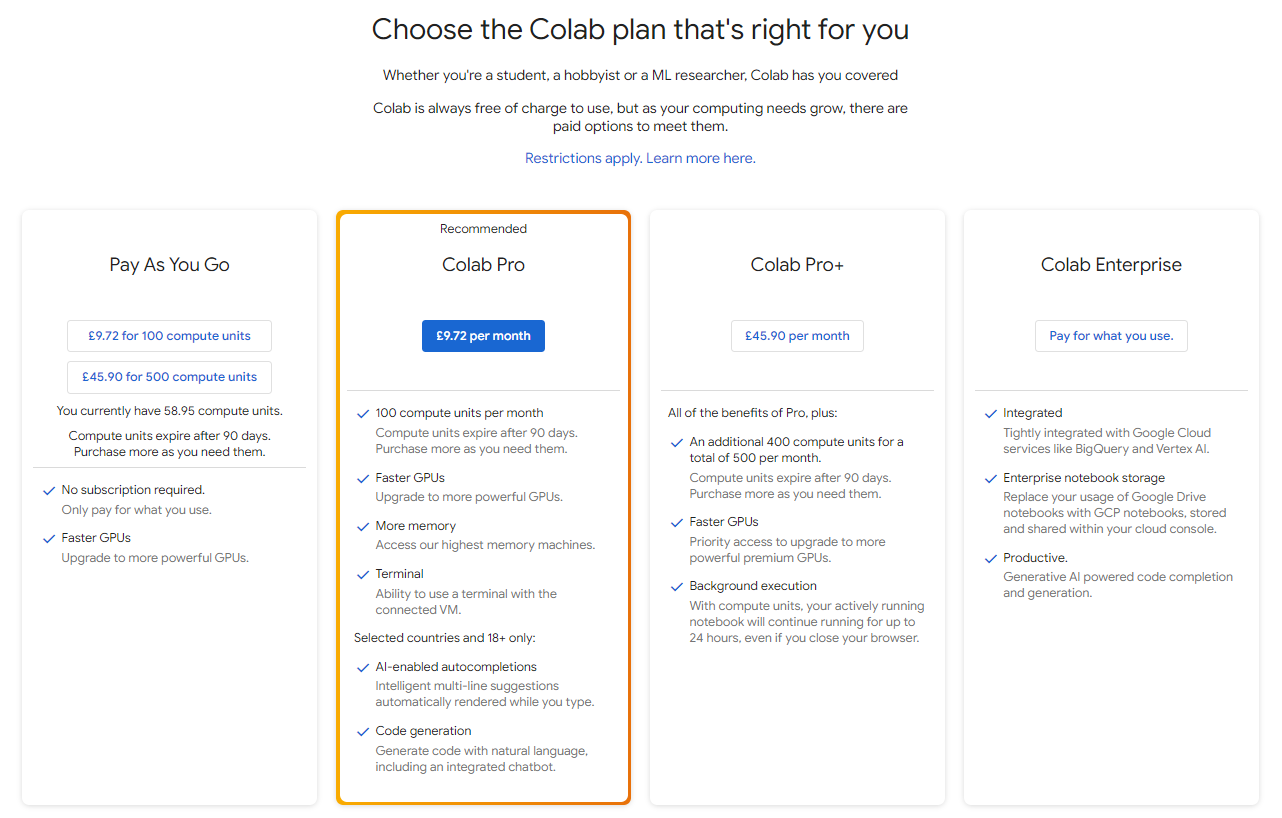
\includegraphics[width=0.7\textwidth]{Google Colab.png}
\caption[A screen-grab of the Google Colab subscription pricing as of March 2024.]{A screen-grab of the Google Colab subscription pricing as of March 2024. Image source: \url{https://colab.research.google.com/signup}.}
\label{fig:Google Colab}
\end{figure}
% -----------COULD REMOVE/CHANGE--------------
Despite its popularity, Google Colaboratory is not flawless. The biggest issue with this software is its steep pricing and quality at certain subscription levels. This section will analyse the question: are these levels worth the money?\\
As shown in Figure~\ref{fig:Google Colab}, there are four primary subscription levels. This analysis will not include ``Colab Enterprise" as this is typically used by larger bodies such as whole companies or research groups.\\
The free version of Colab, not shown in Figure~\ref{fig:Google Colab}, allows execution of small Python programs with a low power \acrshort{gpu}. One major problem with this level is that access to this acceleration is limited by an unspecified number of computation units. After you have used up your units, you are blocked from utilising this \acrshort{gpu} again. Furthermore, a lack of background execution makes this subscription level unstable, with cache eviction causing the webpage to lose the current runtime, along with potential training runs and results. Altogether, this makes the free level of Colab limited, unstable and not suitable for training large \acrshort{ml} models.\\
The ``Pay As You Go" level gives limited access to more powerful \acrshort{gpu}s. The amount of compute units given at this level is often used quickly, especially at the beginning of research when many different things are being trialled. Moreover, Google provides no recovery for interrupted runtimes, meaning that if credits run out halfway through a training run, results can be lost. This results in high money wastage.\\
The ``Colab Pro" level, kindly marked as recommended by Google, is an evil twin to the ``Pay As You Go" level. Although it provides similarly powerful \acrshort{gpu}s, more memory for running sessions and a terminal, it locks users into a subscription. The extra memory is a useful extension as notebooks can occasionally fill up RAM if too much data is loaded or variables are not cleared.\\
``Colab Pro" contains all the disadvantages of ``Pay As You Go" and the benefits are not significant enough to constitute entering into a subscription. Google does at least make it easy to cancel subscriptions\footnote{\url{https://colab.research.google.com/cancel-subscription}}.\\
I recommend utilising “Colab Pro+” as opposed to “Colab Pro”. This subscription level gives a huge 500 compute units, access to the fastest \acrshort{gpu} acceleration and background execution. The pricing of this level also saves at least £2.7 compared to ``Pay As You Go". Background execution saves money, time and effort by preventing runtimes from dying. However, this pricing is still very high, especially if this amount of credits is not required.\\
Overall, Google Colab is a double-edged sword; it is a useful tool, allowing fast development to those without access to hardware acceleration, however, it is an expensive option. Google Colab will not be used for this project due to the pricing and the alternative option of the \acrshort{csf}.\\
% My recommendataion, if Google Colab must be used, is to closely monitor compute unit amounts. ``Colab Pro+"``Colab Pro+" should be used due to its many benefits, downgrading to ``Pay As You Go" as project demand settles in its later stages.
\subsection{Computational Shared Facility}
% ------------COULD REMOVE THIS------------
The \acrfull{uom} \footnote{\url{https://www.manchester.ac.uk/}}, provides a high-performance computing cluster dubbed the \acrfull{csf} \footnote{\url{https://research-it.manchester.ac.uk/services/the-computational-shared-facility-csf/}}. This is provided for primarily staff and PhD students to carry out computationally intensive tasks or jobs requiring possibly hundreds of cores simultaneously.\\
The \acrshort{csf} is a free-to-use resource that staff and students can request access to. It is incredibly fast, consisting of thousands of CPU cores and 100 GPUs such as Nvidia\footnote{\url{https://www.nvidia.com/en-gb/}} V100 Volta and A100 Ampere GPUs.\\
Despite the various possible benefits, many students decide not to use the \acrshort{csf} due to its steep learning curve, batch job system and on-campus requirement.\\
\begin{figure}
\centering
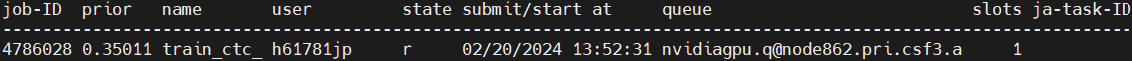
\includegraphics[width=0.9\textwidth]{CSF Example.png}
\caption[A screen-grab from MobaXTerm of a \acrshort{csf} job running.]{A screen-grab from MobaXTerm of a \acrshort{csf} job running. Here the \textit{qstat} command has been used to see the running jobs submitted from the current user. One job is running currently, titled ``train\_ctc\_based.txt".}
\label{fig:CSF Example}
\end{figure}
The \acrshort{csf} is a batch job system, requiring users to submit text files of requested commands and wait for the result. Figure~\ref{fig:CSF Example} shows an example of the job queue for the \acrshort{csf}. Below are listed some of the crucial commands for the \acrshort{csf}:
% ------------COULD REMOVE THIS------------
\begin{itemize}
  \item \textbf{qsub \textit{job\_script.txt}}: Submit a job file to be run
  \item \textbf{qstat}: See the list of jobs you have submitted. They can be listed as \textit{qw} (waiting in the job queue to run), \textit{r} (running) or \textit{Eqw} (Job has errored and will wait forever). If the job has already been completed then this command will show an empty queue
  \item \textbf{qdel \textit{id}}: Stop and delete the job with the ID specified
\end{itemize}
% ------------COULD REMOVE THIS------------
Some major hurdles encountered with the \acrshort{csf} during this project were:
\begin{itemize}
  \item Job files were prepared in Windows, causing an issue. Job files had to be prepared in a Linux format or converted using the \textit{dos2unix} command
  \item Running Juypter Notebook\footnote{\url{https://jupyter.org/}} files automatically required the use of the command \textit{jupyter nbconvert}
  \item Conda environments\footnote{\url{https://conda.io/projects/conda/en/latest/user-guide/tasks/manage-environments.html}} where required to install the correct versions of specific packages
  \item The correct and compatible versions of Cuda and TensorFlow\footnote{\url{https://www.tensorflow.org/install/source}} required installation within this environment
\end{itemize}
% ------------COULD REMOVE THIS------------
The code in Listing~\ref{lst: CSF Job} shows an example of a \acrshort{csf} job script. The script is used to automatically run Juypter notebooks for training.
\begin{lstlisting}[language=Bash, caption={[Example of a CSF job script]{Example of a CSF job script. Here the CSF Juypter module is loaded: this allows Juypter-based commands to be run. Then, the Conda environment is activated and the correct packages are installed and configured, based on debug information from the University. The notebook is then run before the environment is deactivated again.}}, label={lst: CSF Job}]
#!/bin/bash --login
#$ -cwd

#$ -l nvidia_a100=1
module load apps/binapps/jupyter-notebook/6.0.0 #Load Juypter module

source activate myenv #Activate Conda env

#Install correct Cuda and Tensorflow
conda install -y -c conda-forge cudatoolkit=11.8.0
pip install --isolated nvidia-cudnn-cu11==8.6.0.163 tensorflow==2.13.*
conda install -c nvidia cuda-nvcc --yes

#Configure based on information from UoM
CUDNN_PATH=$(dirname $(python -c "import nvidia.cudnn;print(nvidia.cudnn.__file__)"))
export LD_LIBRARY_PATH=$LD_LIBRARY_PATH:$CONDA_PREFIX/lib:$CUDNN_PATH/lib
export XLA_FLAGS=--xla_gpu_cuda_data_dir=$CONDA_PREFIX/lib

#Run the Juypter notebook experiment
jupyter nbconvert --execute --to notebook --ExecutePreprocessor.timeout=-1 --inplace proj_code/colabs/Train\ Video\ Based.ipynb

source deactivate
\end{lstlisting}
The \acrshort{csf} was utilised for this project. The \acrshort{csf} provides 4--5\,GB of RAM for free (with more requiring only a request) compared with Google Colab's 15 GB with more requiring a further subscription. The \acrshort{csf} does have a steep learning curve but it is reliable, scalable, efficient and free compared to Google Colab. The \acrshort{csf} provides the benefits of ``Colab Pro+" without the extreme pricing.\\
An SSH connection was required to access the \acrshort{csf} and submit jobs. However, due to a recent cyber incident, remote access to this network was suspended. Therefore all work was conducted on-campus via the MobaXterm\footnote{\url{https://mobaxterm.mobatek.net/}} application. This allowed for easy control over SHH connections.
\section{Data Generation Pipeline}
\label{sec: Data Generation Pipeline}
This section will outline the process used to generate useful data for training lip reading models and the source dataset selected for training. It will delve into the design decisions and processes employed for data preprocessing.\\
\begin{figure}
\centering
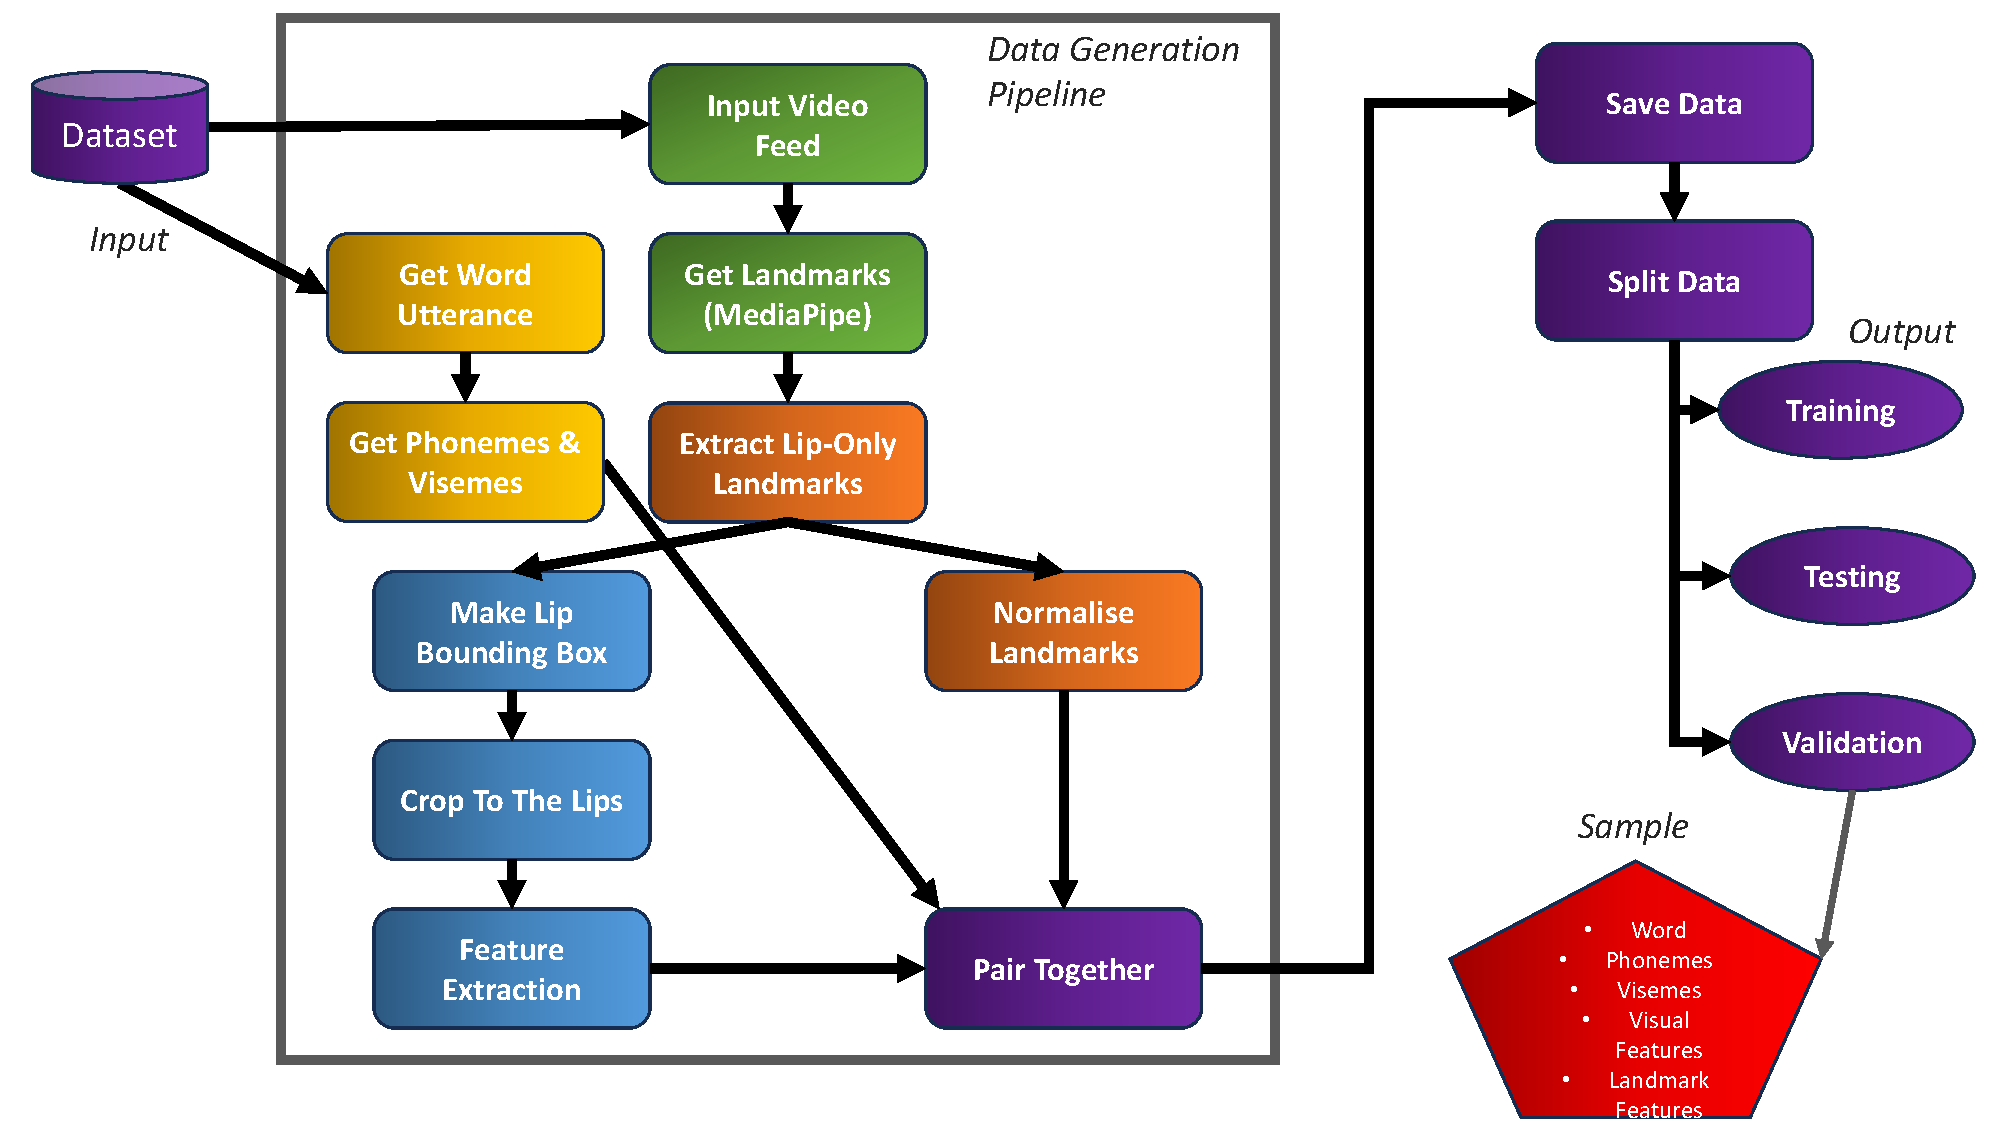
\includegraphics[width=1\textwidth]{Preprocessing Workflow.pdf}
\caption[The Data Generation Pipeline from the LRW data to split samples, ready for training.]{The Data Generation Pipeline from the LRW data to split samples, ready for training. This shows how data samples are constructed for training, combining the labels, visual features and landmark features. All data is preprocessed and saved before a data split is subsequently done.}
\label{fig:Data Gen Pipeline}
\end{figure}
The general process for data generation is shown in Figure~\ref{fig:Data Gen Pipeline}. MediaPipe was applied to each video from the dataset extracting facial landmarks which enabled a crop of the mouth to be taken. Feature extraction was done on the lip crops and the lip landmarks were normalised. This data was stored along with the word, \gls{phoneme} and \gls{viseme} utterances for the video. Data was split into three sets: training, testing and validation.\\
The overall data generation pipeline can be broken down into four primary stages:
\begin{enumerate}
    \item Landmark feature extraction, outlined in Section~\ref{sec: Landmark Feature Extraction}
    \item Visual feature extraction, outlined in Section~\ref{sec: Visual Feature Extraction}
    \item Word utterance processing, outlined in Section~\ref{sec: Word Utterance Processing}
    \item Random data splitting, outlined in Section~\ref{sec: Data Splitting} 
\end{enumerate}
\subsection{Dataset}
\label{sec: LRW Dataset}
For all of these experiments the same dataset and data split were maintained, ensuring consistent results and reliable comparison between the different models.\\
\begin{figure}
\centering
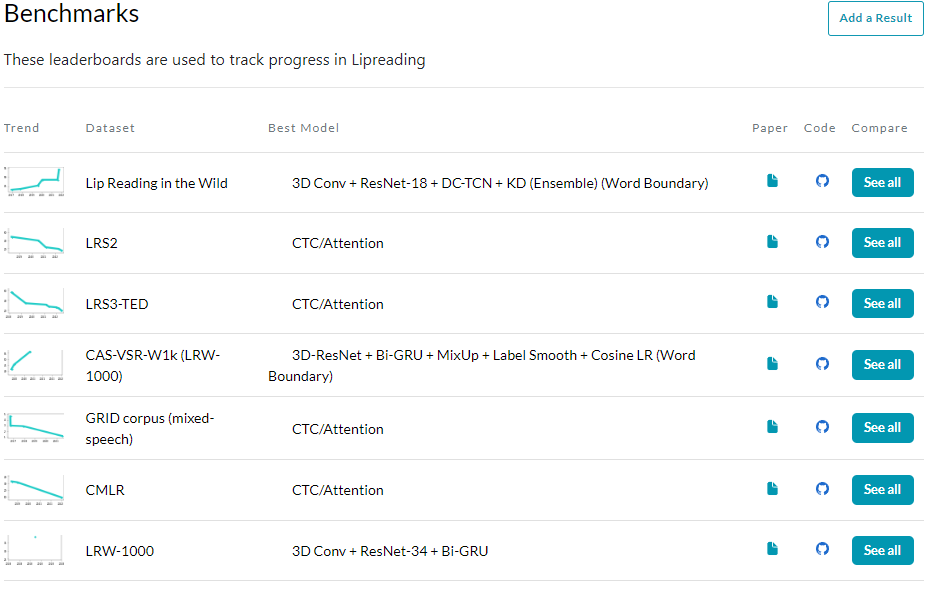
\includegraphics[width=0.7\textwidth]{Lipreading Benchmark.png}
\caption[The benchmark for lip reading via \acrshort{ml}]{The benchmark for lip reading via \acrshort{ml}. This shows some of the available datasets available for training lip reading models. Image source: \url{https://paperswithcode.com/task/lipreading}}
\label{fig:Lip Reading Benchmark}
\end{figure}
Shown in Figure~\ref{fig:Lip Reading Benchmark}, the choice of datasets was primarily between that of \gls{lrw}, \gls{lrs2}, \gls{lrs3}, \gls{lrw1000} and \gls{glips}. The final two of these were not considered because they are transcribed in alternative languages and therefore would pose an additional layer of complexity. Furthermore, \gls{lrs3} was not considered as the data is not available; the link\footnote{\url{https://www.robots.ox.ac.uk/~vgg/data/lip_reading/lrs3.html}} to this data leads to a 404 error.\\
The choice between \gls{lrw} and \gls{lrs2} depends primarily on the task being carried out. Both of these datasets are available upon request online\footnote{\url{https://www.robots.ox.ac.uk/~vgg/data/lip_reading/}}. \gls{lrw} was selected because its structure suits the task being carried out.\\
As shown in Figure~\ref{fig:LRW Structure}, \gls{lrw} consisted of a set of folders named after the primary word utterance within each video. As shown in Figure~\ref{fig:LRW Example 2}, each video consisted of 29 frames from BBC broadcasts. During these clips, a primary word was uttered, but possibly multiple other words were also spoken either before or after the primary utterance.\\
\begin{figure}
\centering
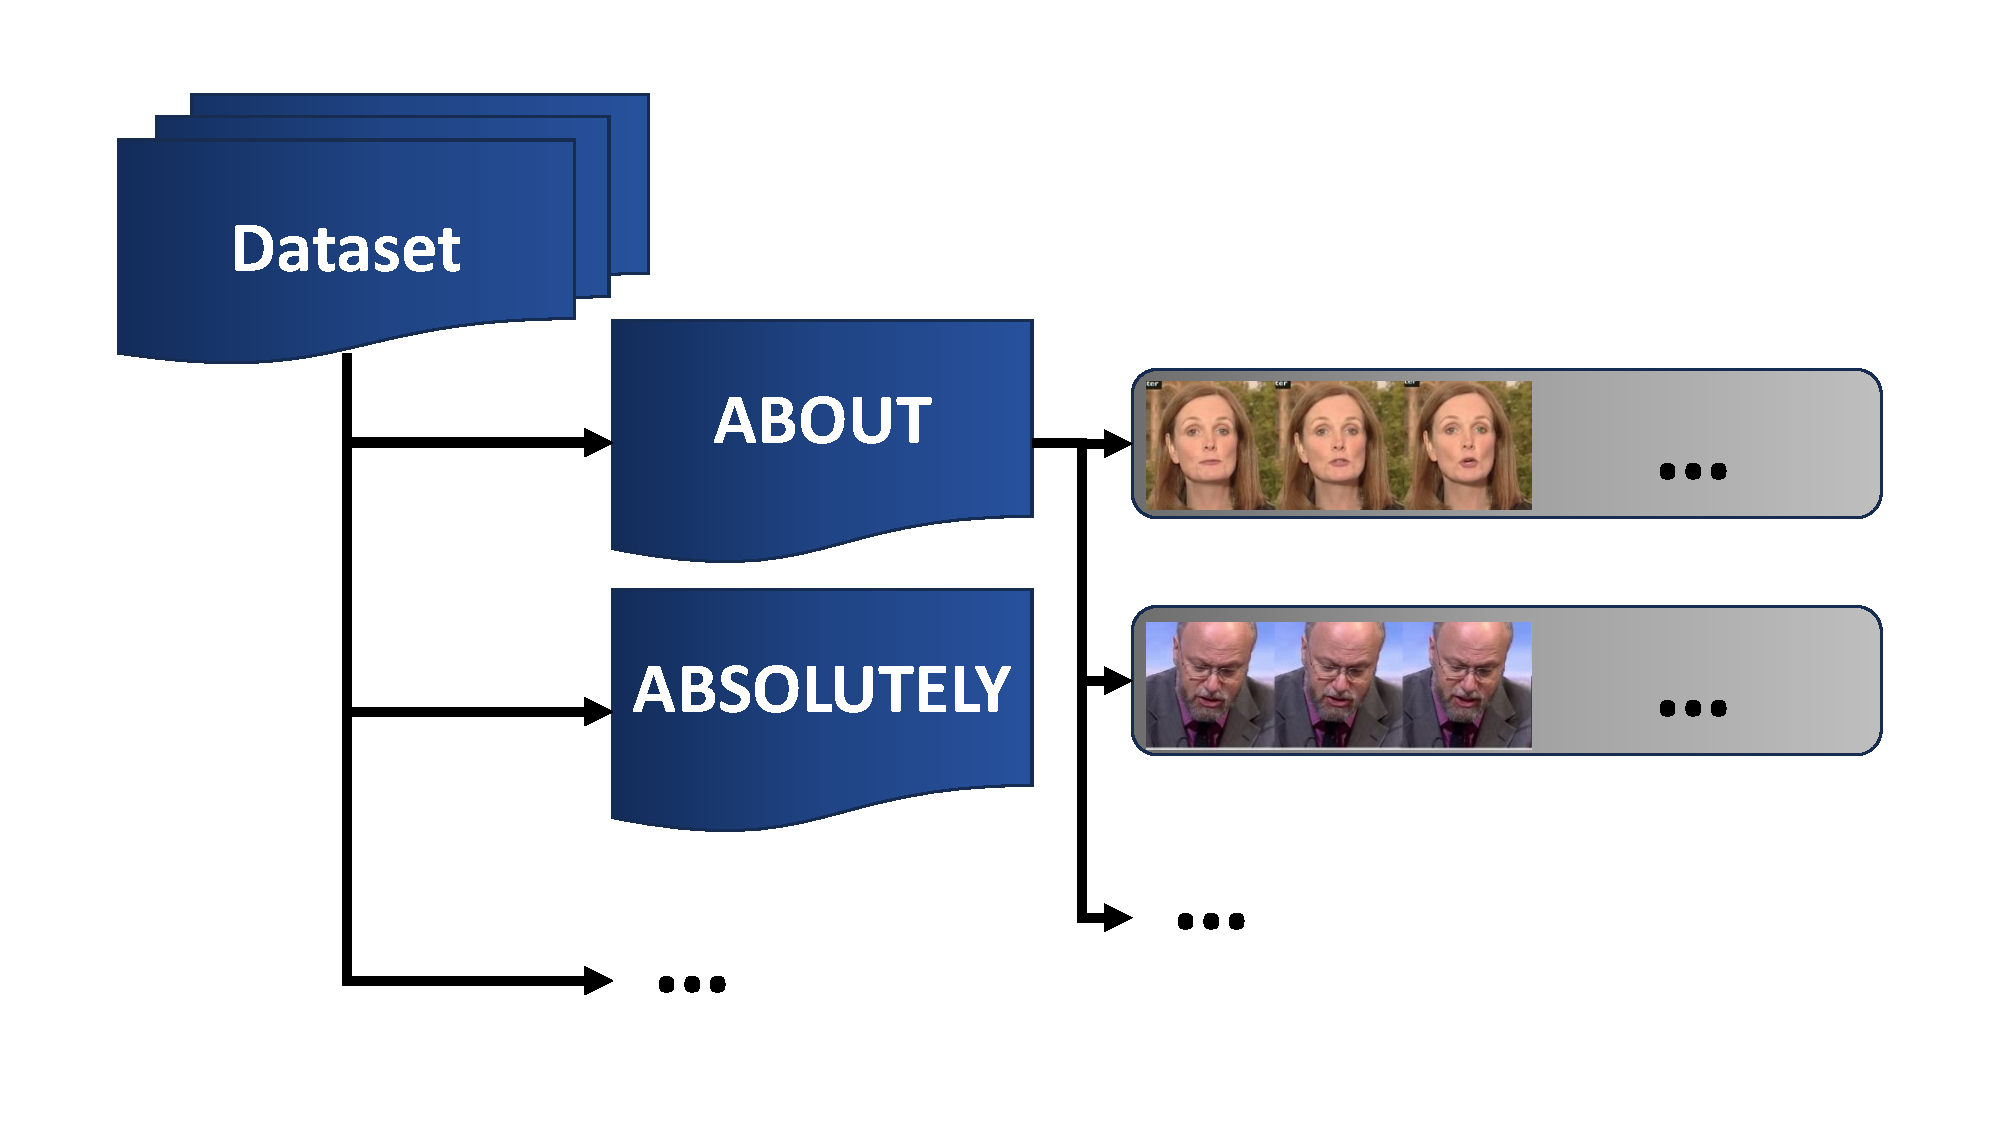
\includegraphics[width=0.7\textwidth]{LRW Structure.pdf}
\caption[The structure of the \gls{lrw} dataset.]{The structure of the \gls{lrw} dataset~\cite{Lip-Reading-In-The-Wild}. \gls{lrw} contains a set of directories labelled with the primary word being spoken. Each directory stores 1100 videos, each 29 frames long of BBC broadcasters saying a small set of words. The primary word spoken is within the middle of the video.}
\label{fig:LRW Structure}
\end{figure}
\begin{figure}
\centering
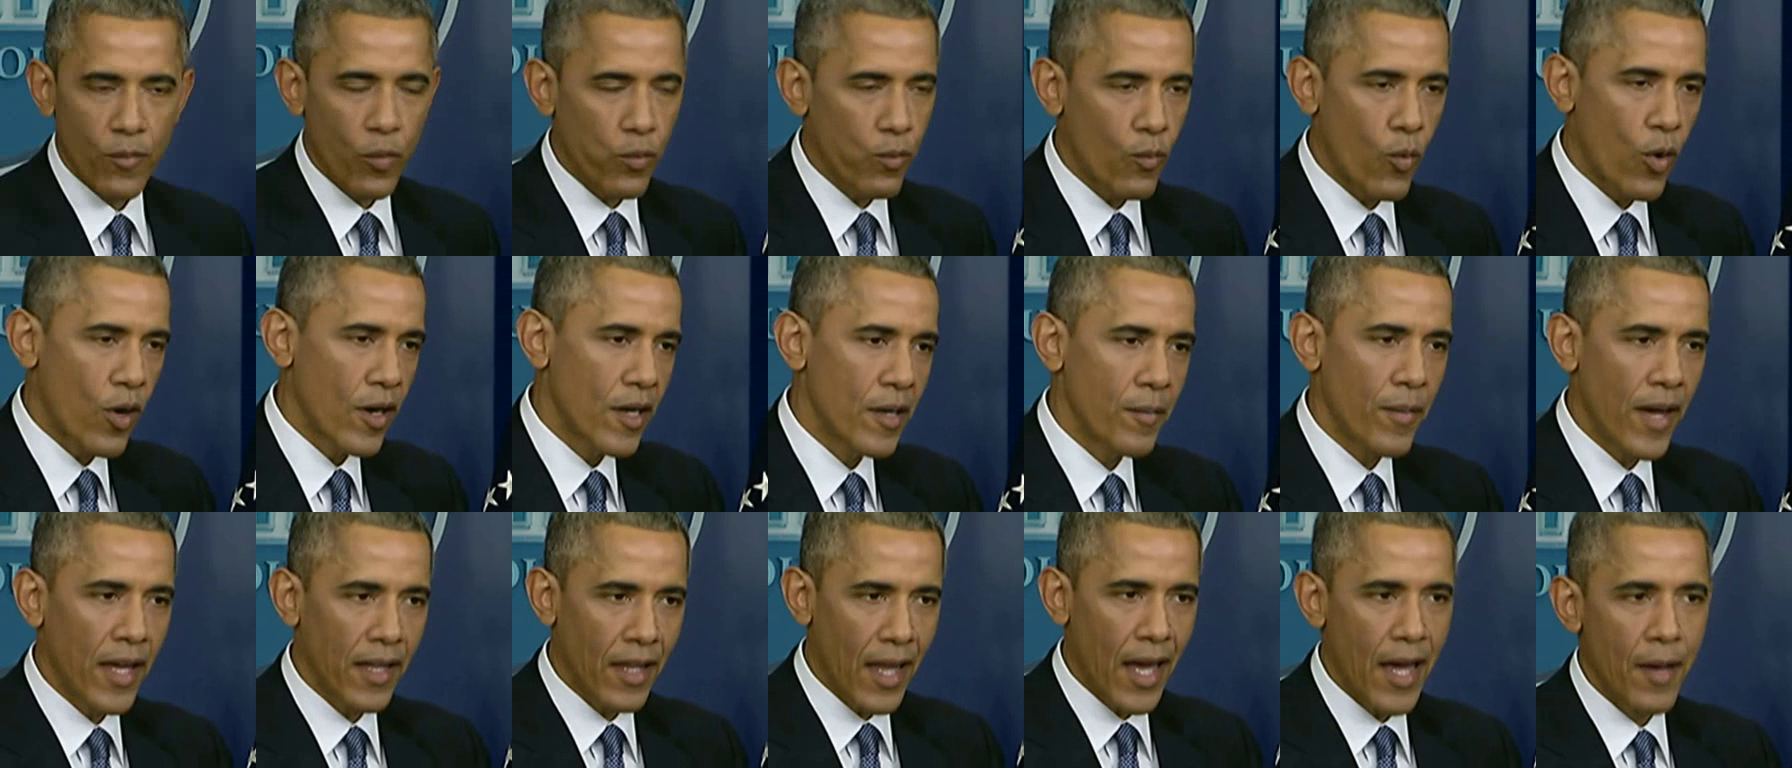
\includegraphics[width=0.7\textwidth]{LRW Example 2.png}
\caption[An extract from the \gls{lrw} dataset.]{An extract from the \gls{lrw} dataset~\cite{Lip-Reading-In-The-Wild}. This clip is labelled as ``ABOUT" but it contains the words ``worried about liability" with the final word half cut off.}
\label{fig:LRW Example 2}
\end{figure}
This structure benefits the model as it provides a large amount of data for each different word utterance, allowing training to fully understand the structure and intricacies of each word. Furthermore, the addition of extra, unlabelled words within clips adds variation to the data and produces models capable of recognising single words within sentences. This is similar to the original research carried out by Chung et al.~\cite{Lip-Reading-In-The-Wild}. The primary downside to \gls{lrw} is the possibility of \gls{overfitting} due to the extra noisy, word utterances.\\ 
The experiments involved training models capable of understanding a small subset of words. \gls{lrw} suited this better compared with \gls{lrs2} which has a collection of random videos, each with a sentence of labelled words. The diversity of words within \gls{lrs2} is useful but not for the task being carried out.\\
Four words were randomly selected for the models to be trained upon: \emph{about}, \emph{believe}, \emph{chance} and \emph{family}. These labels were transformed into \gls{one_hot_encoding}s for training. A subset of words was used to reduce training times and for model comparison. After preprocessing, 4,392 samples of these words were present within the dataset. This is slightly smaller than expected (4400) as MediaPipe could not find a valid face within some images, typically due to the orientation or clipping of faces within frames.\\
To gain access to the \acrshort{lrw} dataset, a request had to be sent to the BBC, explaining the work to be carried out. Once this request was approved, a login was provided for the \acrshort{lrw} website\footnote{\url{https://www.robots.ox.ac.uk/~vgg/data/lip_reading/lrw1.html}}, allowing data to be downloaded.\\
\gls{lrw} was split into seven parts, each approximately 10\,GB in size. Once downloaded, these parts then had to be concatenated together to form a zip file, containing the full dataset. To combine the file sections the command below was run
\begin{lstlisting}[language=Bash, caption={[Commands to combine the sections of the LRW dataset]{Commands to combine the sections of the LRW dataset. Note here that there are two separate sets of commands. The first are the commands presented on the LRW website however, this is seemingly for Linux. The second set is for Windows.}}, label={lst: Extract LRW}]
% Linux Commands:
cat lrw-v1* > lrw-v1.tar
tar -xvf lrw-v1.tar

% Windows Commands:
type lrw-v1* > lrw-v1.tar
\end{lstlisting}
At first these commands caused some issues. As the commands presented for the \acrshort{lrw} dataset are in Linux, and the development system utilised was Windows, some disparity was encountered. Running the commands above in Windows resulted in the file segments being repeatedly combined to form the zip file. After the set was concatenated once, the process was repeated seemingly infinitely.\\
Instead, a different command, shown in Figure~\ref{lst: Extract LRW}, had to be run before 7-Zip\footnote{\url{https://www.7-zip.org/}} was employed to extract these files.
\subsection{Data Preprocessing}
To prepare the data, the videos within \gls{lrw} directories specified as \emph{about}, \emph{believe}, \emph{chance} and \emph{family} were utilised. Each video within these directories was extracted and broken down into 29 individual frames. For each frame, MediaPipe was used to find landmark and visual features. The processes for these methods are detailed in the sections below. Some experiments involved just one of these data types whilst others used both.
\subsubsection{Landmark Feature Extraction}
\label{sec: Landmark Feature Extraction}
\begin{figure}
\centering
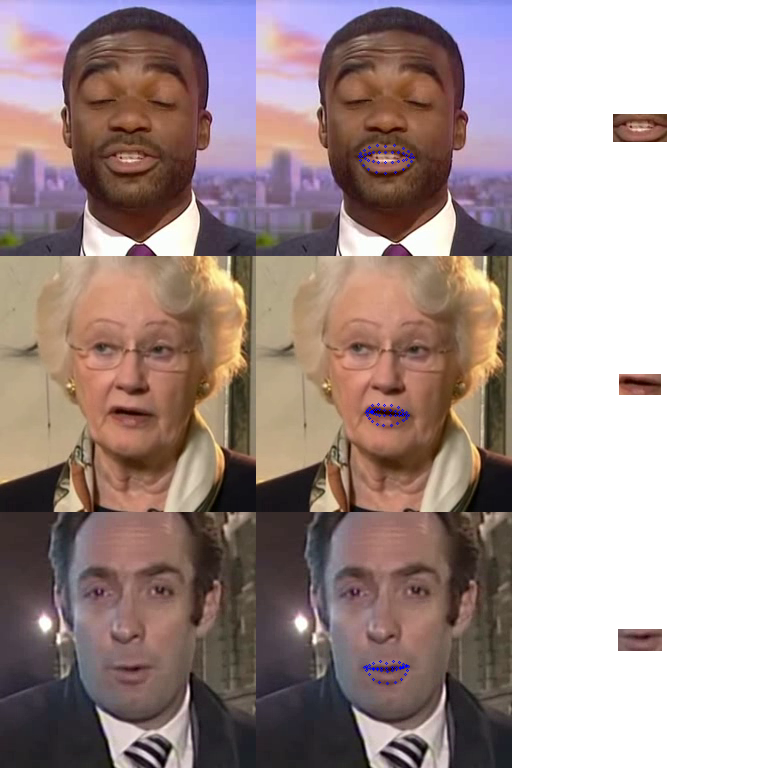
\includegraphics[width=0.7\textwidth]{MediaPipe Example.png}
\caption[An example of using MediaPipe to find the lip landmarks and lip region, from LRW data samples.]{An example of using MediaPipe to find the lip landmarks and lip region, from LRW data samples~\cite{Lip-Reading-In-The-Wild}. Here MediaPipe's Face Landmark Detection was used to generate facial landmarks which were then used to find and crop the lip region. The left images show the default image, the middle with lip-only landmarks highlighted and the right with the subsequent lip crop.}
\label{fig:MediaPipe Example}
\end{figure}
Explored in Section~\ref{sec:mediapipe}, MediaPipe provides a Face Landmark Detection\footnote{\url{https://mediapipe-studio.webapps.google.com/demo/face_landmarker}} model. This model was used to generate a set of 478 facial landmarks for each frame of the data subset used. Forty of these landmarks, specified in Listing~\ref{lst: MediaPipe Lip Indices}, corresponded to parts of the lips, so were extracted and used for training. Examples of this extraction process can be seen within Figure~\ref{fig:MediaPipe Example} and Figure~\ref{fig:Landmark Example}\\
\begin{figure}
\centering
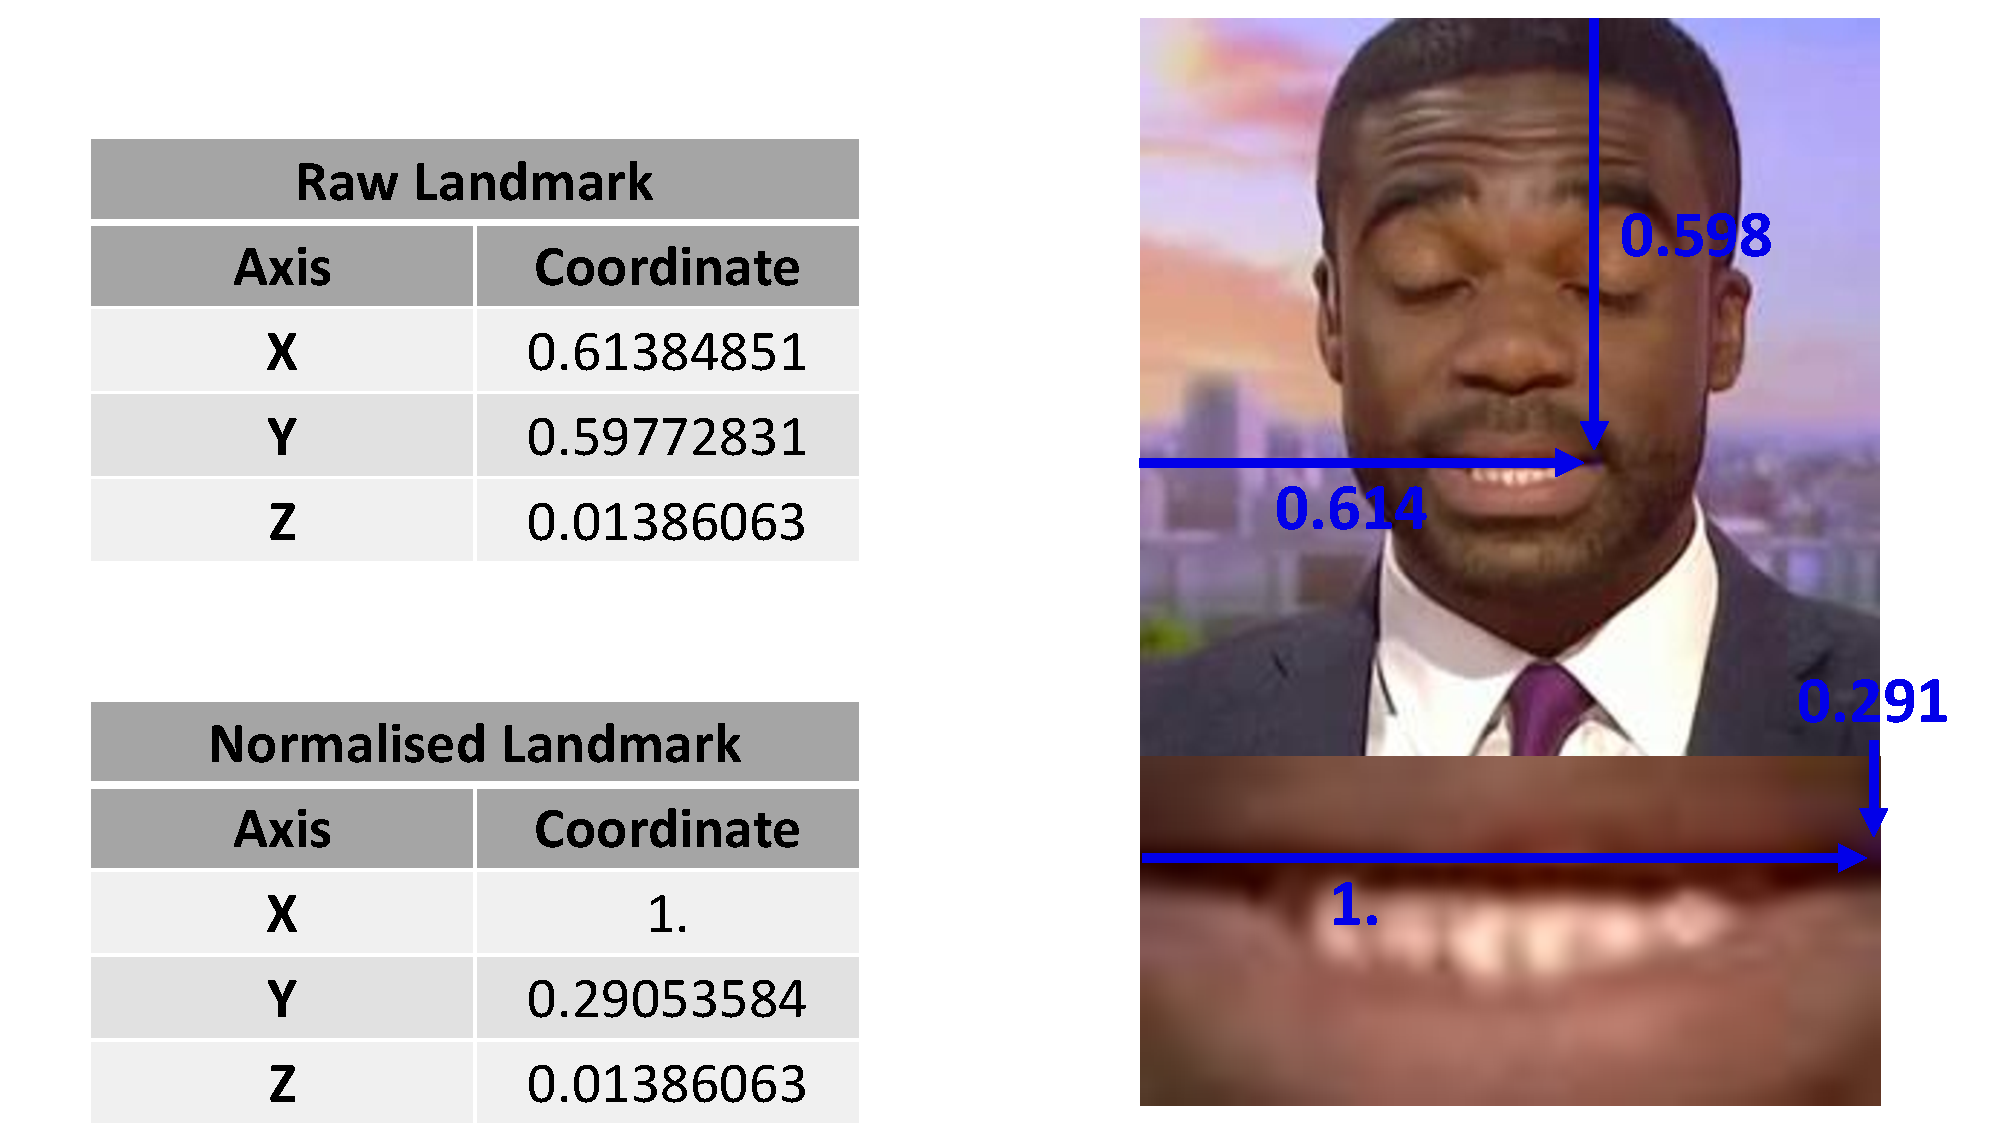
\includegraphics[width=0.7\textwidth]{Landmark Example.pdf}
\caption[An example of a normalised MediaPipe landmark]{An example of a normalised MediaPipe landmark, from the \gls{lrw} data samples~\cite{Lip-Reading-In-The-Wild}. Here MediaPipe is used to find facial landmarks. A single landmark is observed, which is displayed on the full image and the lip crop. The landmark is normalised based on the whole lip crop.}
\label{fig:Landmark Example}
\end{figure}
Landmarks are sets of $(X, Y, Z)$ coordinates relative to the position of facial landmarks within images. This is unsuitable for training as variation in the global position of faces within the video feeds can cause underfitting and make lip reading results incomparable. Therefore, normalisation was used to transform these coordinates into a proportionate form.\\
\begin{lstlisting}[language=Python, caption={[A list of the MediaPipe facial landmarks that correspond to the lips.]{A list of the MediaPipe facial landmarks that correspond to the lips. These correspond to the indices visualised within Figure~\ref{fig:mediapipe landmarks} as the facial landmarks associated with the lips.}}, label={lst: MediaPipe Lip Indices}]
lip_landmarks_outer_keys: typing.List[int] = [
    61, 185, 40, 39, 37, 0, 267, 269, 270, 409, 291, 375, 321, 405, 314, 17, 84, 181, 91, 146,
]
lip_landmarks_inner_keys: typing.List[int] = [
    78, 191, 80, 81, 82, 13, 312, 311, 310, 415, 308, 324, 318, 402, 317, 14, 87, 178, 88 95,
]
\end{lstlisting}
The mathematical function for this normalisation is shown below
\[X_i = \frac{X_i - X_l}{w},\]
\[Y_i = \frac{Y_i - Y_l}{h},\]
\[Z = Z,\]
where $(X_l, Y_l, 0)$ corresponds to the upper left coordinate of a bounding box created using all of the lip landmarks (defined in Section~\ref{sec: Visual Feature Extraction}), $(X_i, Y_i, 0)$ correspond to the coordinates of the $i$th lip landmark, and $w$ and $h$ are the width and height respectively of the lip bounding box in the image.\\
The width, $w$, and height, $h$, of the lip bounding boxes were formulated using the equations below
\[w = \max\{X_1, X_2,...X_{40}\} - \min\{X_1, X_2,...X_{40}\},\]
\[h = \max\{Y_1, Y_2,...Y_{40}\} - \min\{Y_1, Y_2,...Y_{40}\}.\]
The $Z$ coordinate was not normalised as this represents the depth of a landmark within an image. Thus, it is less useful for training and not relative to the image coordinates.\\
Once the landmarks were normalised they were saved to the preprocessed dataset.
\subsubsection{Visual Feature Extraction}
\label{sec: Visual Feature Extraction}
Landmark features are not enough on their own. There is substantial, relevant data related to speech that is not captured by the placement of the lips alone. For example, the teeth and tongue are both key to distinguishing certain \gls{phoneme}s yet not captured by MediaPipe. Utilising wider visual features is a technique adopted by various other successful lip reading systems~\cite{Lip-reading-techniques} and has been proven to produce better results~\cite{lipreading_with_attention}.\\
To produce visual features, the lip landmarks extracted in the previous stage were reused to create a bounding box around the lips. This bounding box was used to take a crop of each frame of the videos from \gls{lrw}.\\
To find the bounding box, defined by the coordinates $(X_l, Y_l)$ (for the top left corner) and $(X_r, Y_r)$ (for the bottom right corner), the following calculations were carried out:
\[X_l = \min(X_1, X_2,...X_{40})\]
\[Y_l = \min(Y_1, Y_2,...Y_{40})\]
\[X_r = \max(X_1, X_2,...X_{40})\]
\[Y_r = \max(Y_1, Y_2,...Y_{40})\]
Where $X_i$ defines the $X$ coordinate of lip landmark $i$ and $Y_i$ defines the $Y$ coordinate of lip landmark $i$.\\
InceptionV3 Imagenet \footnote{\url{https://keras.io/api/applications/inceptionv3/}}~\cite{InceptionV3} was used for visual \gls{feature_extraction} of the lip crops.\\
InceptionV3 Imagenet is lightweight and has high performance, making it useful for devices that might not use a GPU, whilst still boasting very high accuracy~\cite{InceptionV3}. It has a straightforward implementation via Keras. Possible future work could aim at experimenting with alternative feature extractors to compare performance metrics.\\
As shown in Figure~\ref{fig:Visual Feature Extraction}, lip crops were passed through the InceptionV3 Imagenet feature extractor, generating 2048 long feature vectors. Visual features were paired with the corresponding landmark features before being saved.
\begin{figure}
\centering
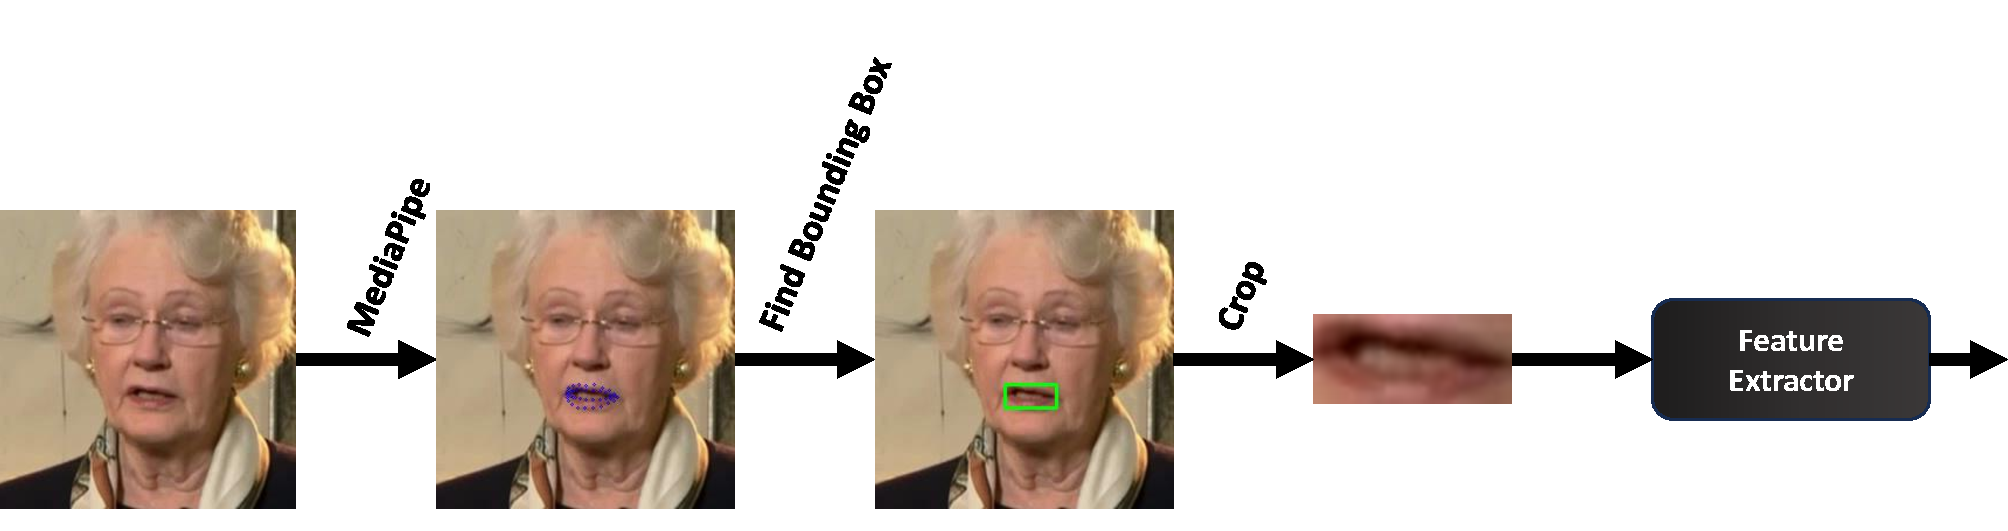
\includegraphics[width=0.7\textwidth]{Visual Feature Extraction.pdf}
\caption[The process of visual feature extraction.]{The process of visual feature extraction. MediaPipe is used to find lip landmarks. A bounding box is made surrounding all landmarks before a crop is taken. The crop is passed into a feature extractor.}
\label{fig:Visual Feature Extraction}
\end{figure}
\subsection{Word Utterance Processing}
\label{sec: Word Utterance Processing}
During training, videos were classified into a set of different classes:
\begin{itemize}
    \item The \textbf{words} spoken: \gls{multi-class} and \gls{single-label}
    \item The \textbf{letters} of words spoken: \gls{multi-class} and \gls{multi-label}
    \item The \textbf{\gls{phoneme}s} uttered: \gls{multi-class} and \gls{multi-label}
    \item The \textbf{\gls{viseme}}s expressed: \gls{multi-class} and \gls{multi-label}
\end{itemize}
\Gls{lrw} is currently annotated with only the words (and, therefore, also the letters) spoken within videos. Thus, both the \gls{phoneme}s and \gls{viseme}s for these had to be generated automatically.\\
To produce the \gls{phoneme}s, from words, the Python library NLTK\footnote{\url{https://www.nltk.org/_modules/nltk/corpus/reader/cmudict.html}} was used. Described in Section~\ref{sec: nltk}, this library can be used to convert words into their constituent \gls{phoneme}s via the Carnegie Mellon Pronouncing Dictionary (cmudict).\\
\begin{figure}
\centering
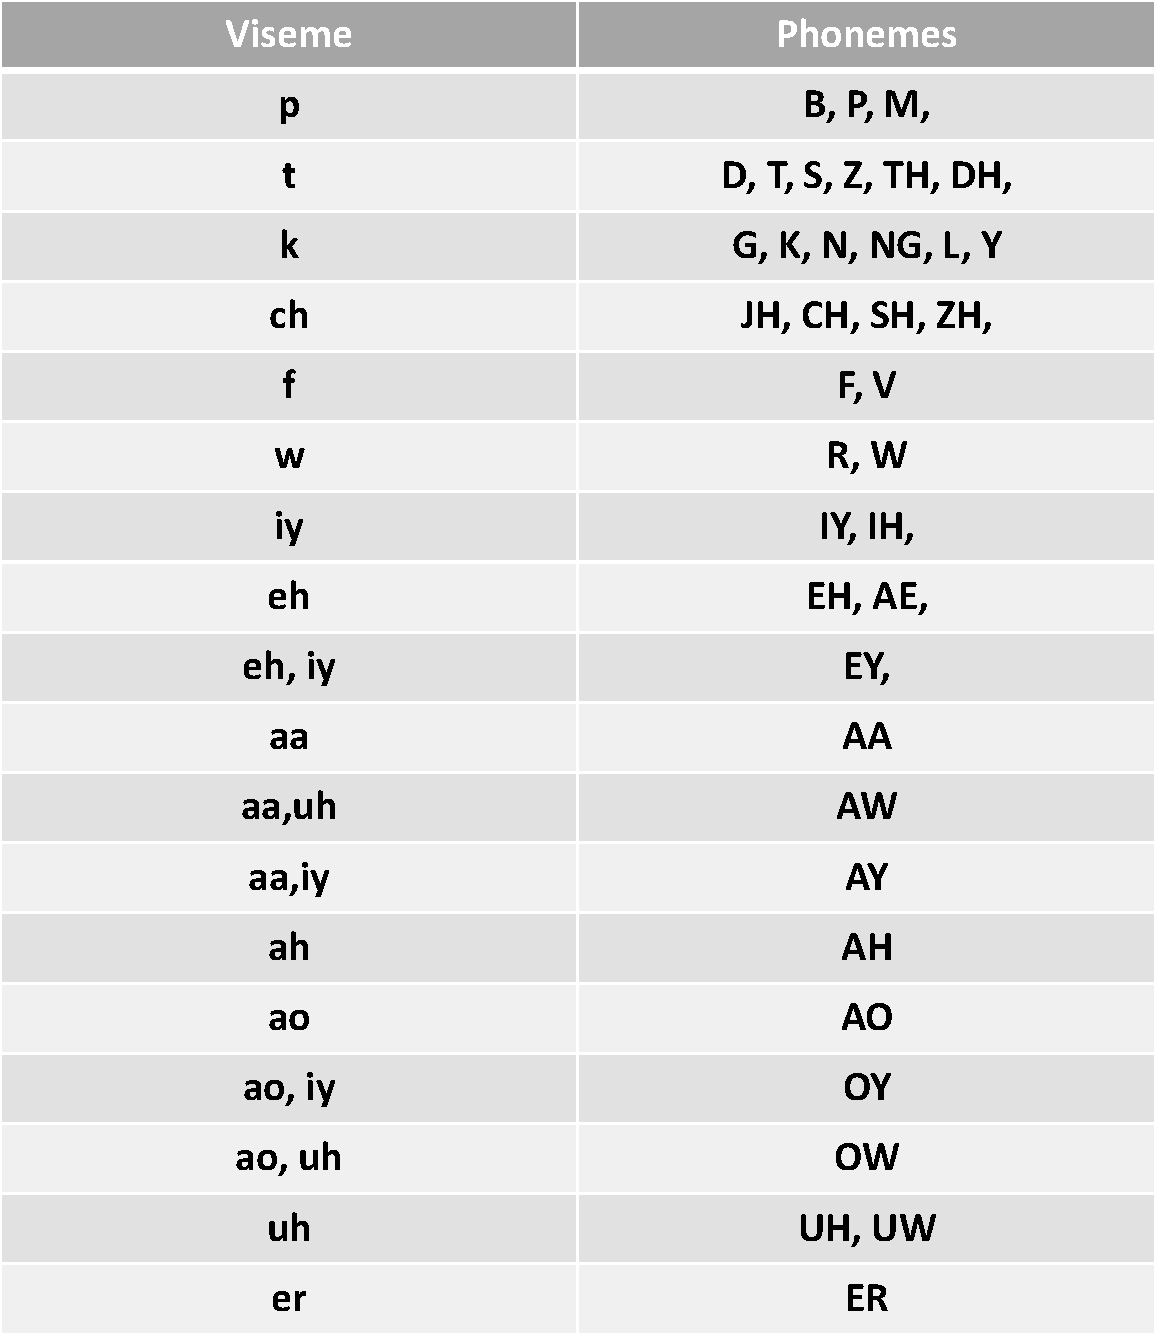
\includegraphics[width=0.7\textwidth]{P2V Mapping.pdf}
\caption[The adopted \acrshort{p2v} mapping, as proposed by Lee et al. and promoted by Bear et al.]{The adopted \acrshort{p2v} mapping, as proposed by Lee et al.~\cite{best_phoneme_viseme_mapping} and promoted by Bear et al.~\cite{phoneme_viseme_mapping_review}. This shows which \gls{phoneme}s fall into each \gls{viseme} group. Some \gls{phoneme}s are made up of multiple \gls{viseme}s and are therefore marked as such. There are thirteen \gls{viseme}s in total (and an additional blank \gls{viseme}, although this has not been added above).}
\label{fig:P2V Mapping}
\end{figure}
As explained more in Section~\ref{sec: Lip Reading}, retrieving the \gls{viseme}s of words is a harder task. Classification based on \gls{viseme}s is potentially a more fruitful endeavour for classification; \gls{viseme}s relating more closely to the visual aspects of language compared with letters or \gls{phoneme}s. However, there currently exists no defined \gls{viseme} set, let alone a tool for \acrfull{p2v} conversion.\\
For this set of experiments, as suggested by Bear et al.~\cite{phoneme_viseme_mapping_review}, the \acrshort{p2v} mapping proposed by Lee et al.~\cite{best_phoneme_viseme_mapping} was employed for \acrshort{p2v} conversion. This is shown within Figure~\ref{fig:P2V Mapping}. Note that some of the \gls{phoneme}s have two overlapping \gls{viseme}s (such as ``EY" and ``AW"). Although Lee et al.~\cite{best_phoneme_viseme_mapping} do not elaborate upon this, the reason for this is likely that some \gls{phoneme}s required multiple \gls{viseme}s to express.\\
\Gls{phoneme}s were converted into \gls{viseme}s using a Python dictionary. Once words had equivalent phonetic and visual forms, these data labels were exported with the corresponding data samples.
\subsection{Data Splitting}
\label{sec: Data Splitting}
\begin{figure}
\centering
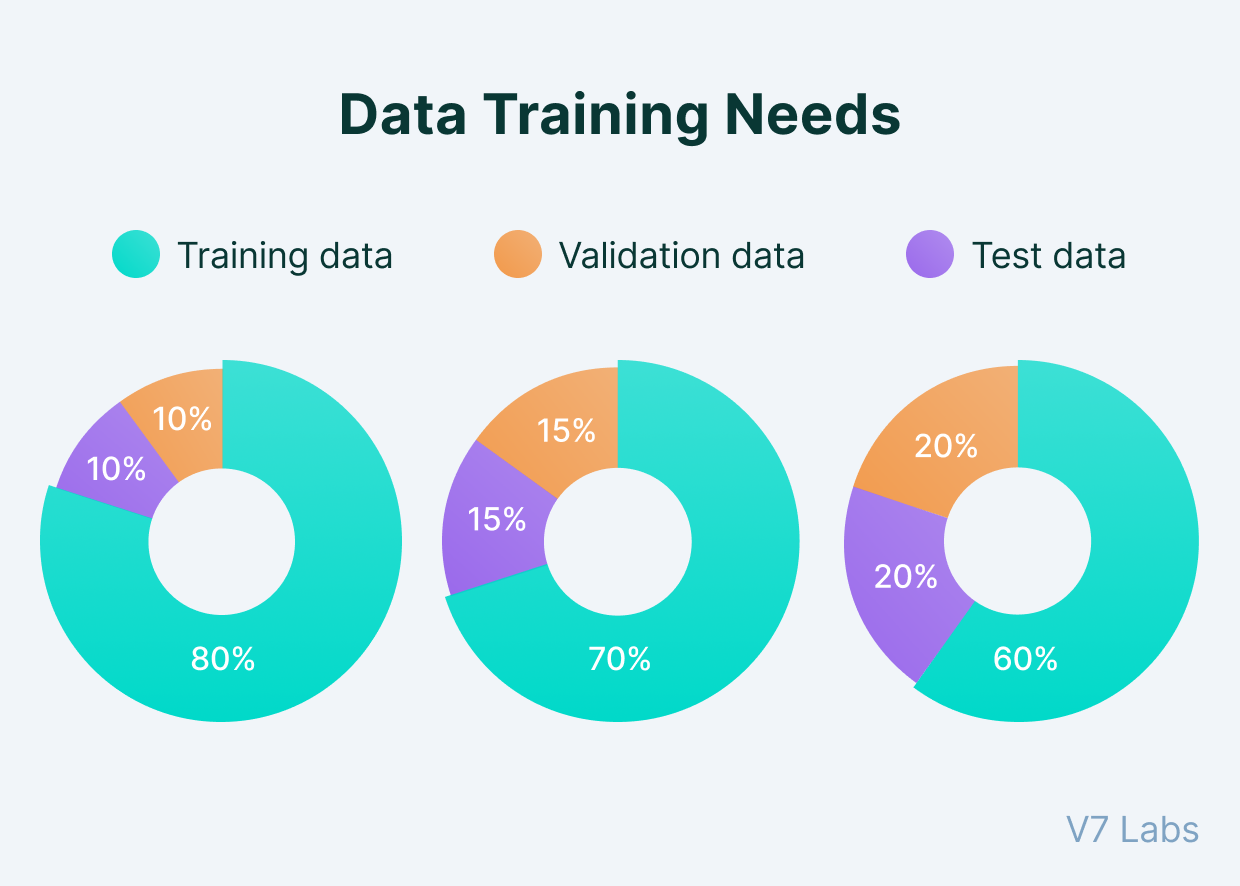
\includegraphics[width=0.5\textwidth]{Data Split Diagram.png}
\caption[A diagram of some common data split ratios used in \acrfull{ml}.]{A diagram of common data split ratios used in \acrfull{ml}.}
\label{fig:Data Split}
\end{figure}
Data splitting refers to the process of separating data into multiple sets, one to train the \acrshort{ann} and another to evaluate it~\cite{Data-Splitting_2}.\\
There are three typical sets for data splitting: training, testing and validation. The training set is used to train and optimise the model's parameters. The validation and testing sets are used to provide an unbiased view of the model's performance, kept separate to prevent \gls{overfitting}. The validation set is used to evaluate the model's performance and fine-tune its hyperparameters throughout training. The testing set is used to evaluate the model's final, overall performance and to directly compare different models.\\
There are various methods of data splitting, including but not limited to \acrfull{srs}, trial-and-error and systematic sampling~\cite{Data-Splitting}. These methods for data splitting primarily affect the variance of the model error. For example, trial-and-error sampling estimates the model error with lower variance than other methods~\cite{Data-Splitting}. For this research, the simple and easy-to-implement \acrshort{srs} was utilised during training, testing and validation even despite its high variance.\\
As shown in Figure~\ref{fig:Data Split}, there are different proportions of data split. Here data was split by randomly shuffling the data samples and selecting the first 80\% of samples for training, the next 10\% for testing and the final 10\% for validation. This is a common data split used within \acrshort{ml} projects.
\section{Design of Experiments}
This section will cover the structure of experiments covered within this research, including the many different design decisions and principles followed.
\subsection{Experiment Structure}
\begin{figure}
\centering
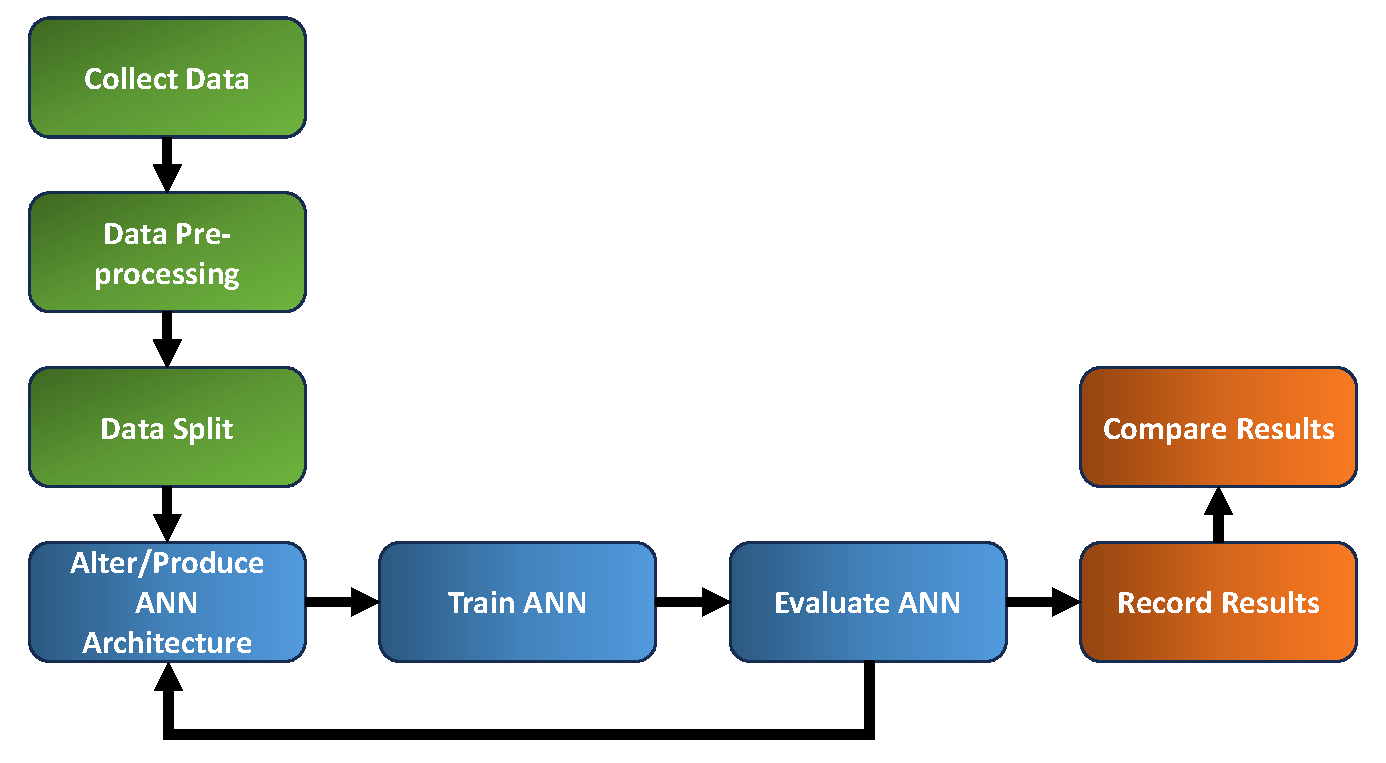
\includegraphics[width=0.7\textwidth]{Experiment Workflow.pdf}
\caption[The workflow adopted within the experiments.]{The workflow adopted within the experiments. The green section shows the steps that were carried out first and only once. The blue section was repeated several times, for each experiment. This section shows the iterative nature of the experiments, where changes are repeatedly made to gather further results. The orange section shows the critical reflection within this research.}
\label{fig:experiment workflow}
\end{figure}
The experiment structure is a key design decision that will inform the reliability of results and help to better compare alternative lip reading architectures. This structure is depicted in Figure~\ref{fig:experiment workflow}.\\
After data was collated and preprocessed, a set of experiments were carried out. The \acrshort{ann} was repeatedly altered, trained and evaluated to study the impact that various hyperparameters had on lip reading.\\
Models were trained using the training and validation sets, employing early stopping as specified within Section~\ref{sec: Early Stopping}. For each experiment, the optimal models were loaded back in and run against the testing dataset. This was used to objectively capture the performance on unseen data. The accuracy, loss and \acrfull{wer} (as defined in Section~\ref{sec: JiWER}) were observed.\\
Models were compared via their validation and testing metrics to find the best hyperparameter settings and draw conclusions as to the difficulties or benefits of different methods.\\
% Eg. Varying only 1 thing at a time. Finding the accuracy, loss & comparing them.
There were three principles fostered for these experiments:
\begin{itemize}
    \item Maintain the data split
    \item Make single changes between experiments --- changes can be large or small
    \item Maintain optimal changes to produce increasingly optimal models
\end{itemize}
The first concern is that of data. To allow for better model comparison, the same data sets should be employed to train and then evaluate the different models. This makes them directly comparable. Therefore, the data split algorithm was incorporated into the data generation pipeline, maintaining the split between the different experiments. This had the benefit of saving computation and processing by avoiding repeated, redundant data splits. The data split was made on each word class individually rather than the entire dataset. This ensured similar quantities of each data class for training, testing and validation.\\
The next concern is how to compare different experiments. Typically, only one thing should be varied between experiments to ensure that any changes in performance can be attributed directly to the change made. This is a hard task for \acrshort{ml}, where many different parameters are at play. Furthermore, this is made difficult by the definition of what a ``single change" entails: is this a single parameter change or a whole different \acrshort{ann} architecture? Early stopping, explained further in Section~\ref{sec: Early Stopping}, means that models could be trained for varying numbers of epochs which adds further variation. For this research, only one thing was purposefully altered, for example batch size or \acrfull{lr}. Changes between experiments could be more extensive, such as trying a whole different model architecture, but these changes were fully documented for this reason. Variation due to early stopping could not be avoided compared with the potential benefit this method poses to the performance of models.\\
The final principle is maintaining optimal changes to models where possible. When beneficial changes were discovered, these were maintained between experiments. This ensured an increasing performance throughout.
\subsection{Early Stopping}
\label{sec: Early Stopping}
For all training runs, early stopping was employed to save the best model weights. This was achieved using Keras's callback, ModelCheckpoint\footnote{\url{https://keras.io/api/callbacks/model_checkpoint/}}. This was configured to monitor the validation loss and save the model with the best performance. This would ensure the model is saved before \gls{overfitting} occurs and metrics worsen.
\subsection{Learning Rate}
\label{sec: Learning Rate}
The Adam optimiser was used in conjunction with exponential decay during training. Exponential decay was utilised to decay the \acrshort{lr} over time, as the local minimum was approached, thus scaling Adam's effect over time.\\
Adam, or adaptive moment estimation optimiser, is a modern \acrshort{lr} scheduler made popular due to its effectiveness, simplicity and handling of large amounts of data~\cite{Adam_OG}. In addition, Keras provides an easy-to-use Adam optimiser\footnote{\url{https://keras.io/api/optimizers/adam/}}. Adam works by selectively adjusting the \acrshort{lr} for each parameter, based on the history of that parameter~\cite{Adam_OG}.\\
Exponential decay is a method of lowering \acrshort{lr} over time, based on the current epoch. The benefit of using a decay is that a higher initial \acrshort{lr} can be employed at first, preventing \acrshort{ann}s from learning noisy data. The \acrshort{lr} is then reduced throughout, as the model converges to a global minimum in the loss. This reduces the negative impact on model performance during the early stages of training~\cite{benefit_of_decay}. Exponential decay is a popular and simple method of this, as defined below
\[lr_{new} = lr_{initial} \cdot e^{-D \cdot n},\]\\
where $lr_{new}$ is the updated \acrshort{lr} for the current epoch $n$, $lr_{initial}$ is the initial \acrshort{lr} and $D$ is the decay rate. The decay rate is a further parameter introduced with exponential \acrshort{lr} decay, used to control the rate of change.\\
In Keras, exponential decay\footnote{\url{https://keras.io/api/optimizers/learning_rate_schedules/exponential_decay/}} is configured with four different parameters. The $``decay\_rate"$ and $``initial\_learning\_rate"$ are easier to understand but for $``decay\_steps"$ and $``staircase"$ this is less the case. Keras gives the following function to define their formulation\\
\[LR = initial\_learning\_rate \times decay\_rate^{(step/decay\_steps)},\]
where $step$ is the number of total steps. This formulation is controlled by $``staircase"$ which controls the type of division used within the exponential $(step/decay\_steps)$. When set to false, this formulation will be true division, resulting in a continuous change to the \acrshort{lr}. But $``staircase"$ is set to true, integer division is employed, resulting in a discrete, staircase-like change in the \acrshort{lr}.\\
For the experiments that employ exponential decay, $``staircase"$ will be set to false, resulting in this continuous change to the \acrshort{lr}. The $``decay\_steps"$ will be configured based on the amount of data samples and the batch size. A formulation for this is defined below.
\[decay\_steps = \frac{total\_training\_samples}{batch\_size}.\]
This ensures that all samples are utilised exactly once during each training epoch.
\section{Graphical User Interface}
\label{sec: gui}
The \acrfull{gui} integrates the features of the data generation pipeline, outlined in Section~\ref{sec: Data Generation Pipeline}, and a subset of the models trained in Chapter~\ref{cha:results}. It brings these elements together to better showcase the system as a whole and test the lip reading system in practise.
\subsection{Inference Workflow}
\begin{figure}
\centering
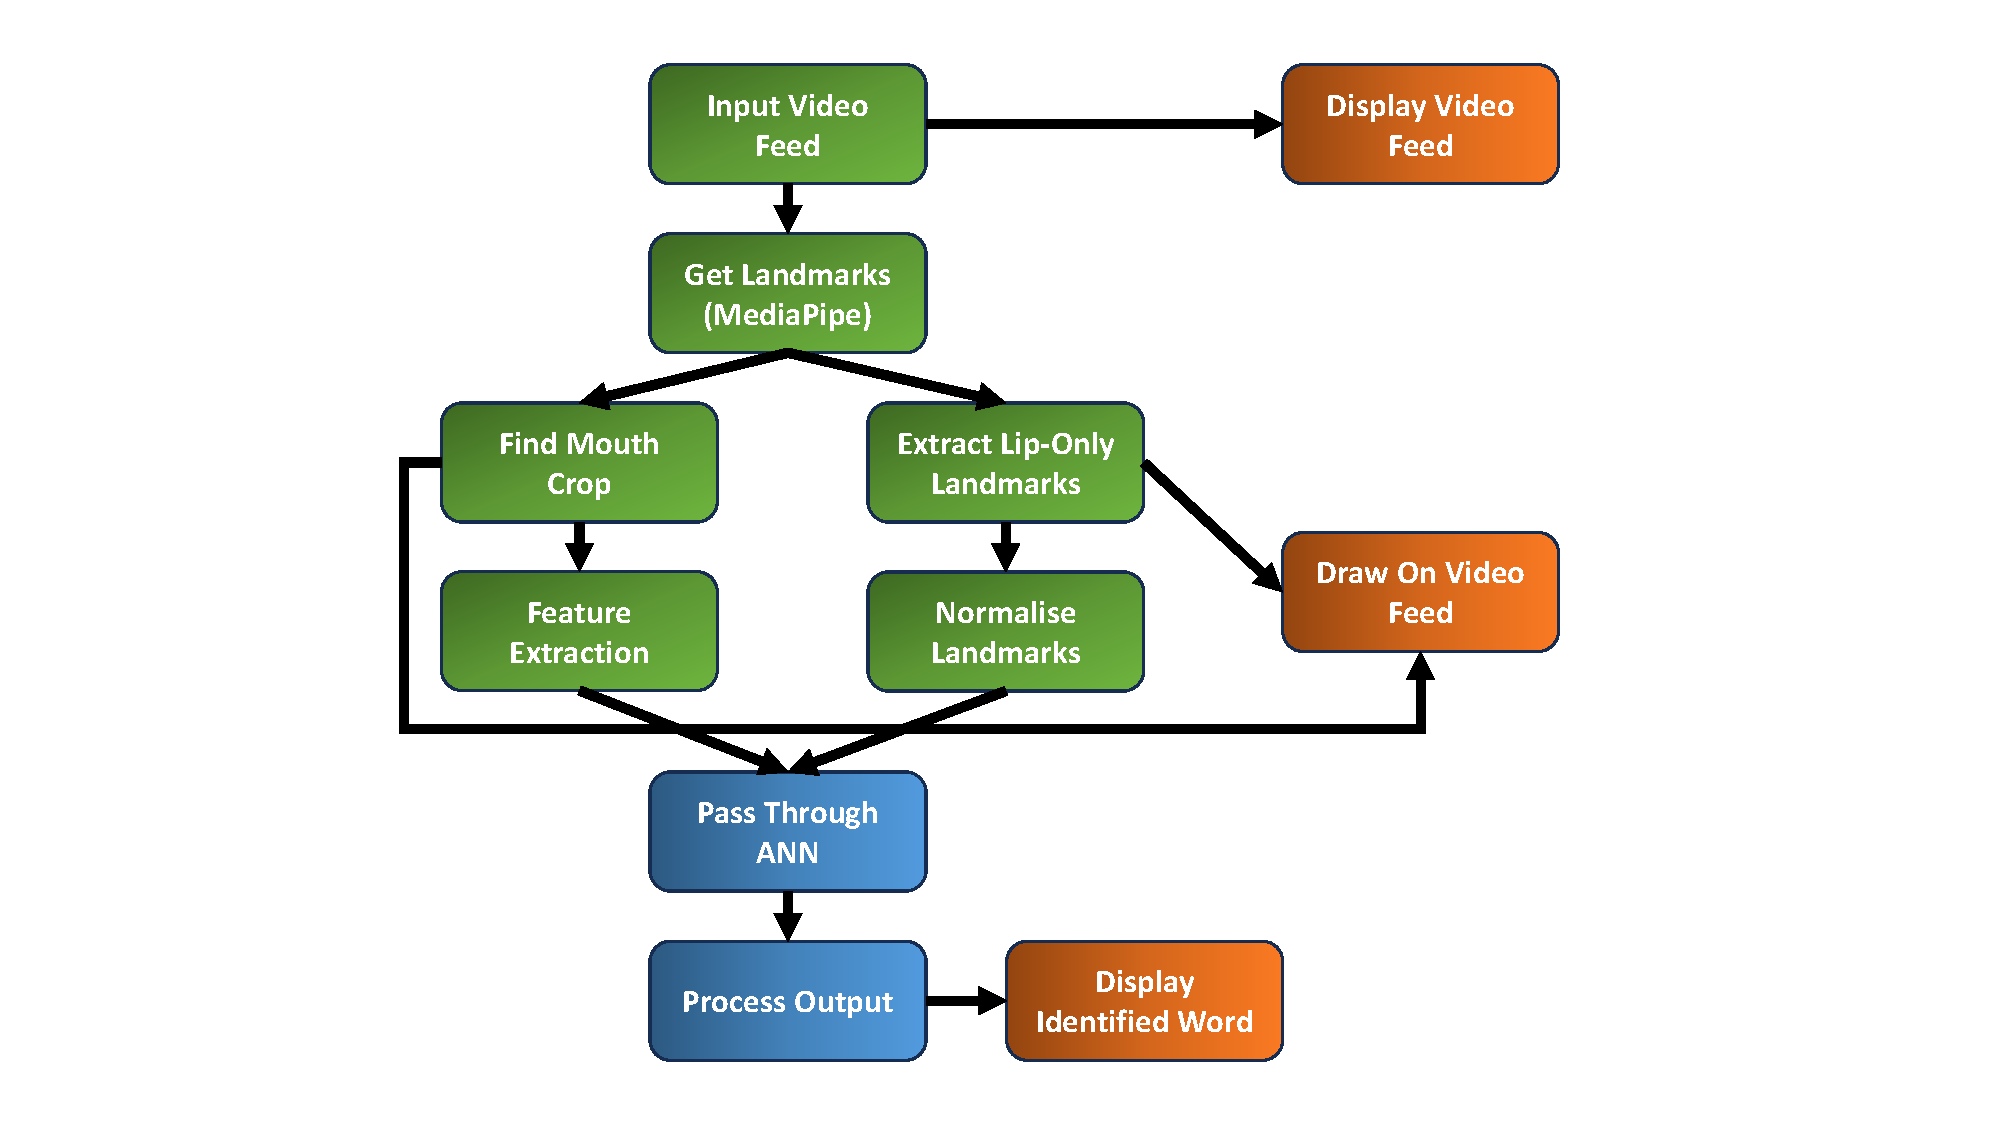
\includegraphics[width=1\textwidth]{GUI Workflow.pdf}
\caption[Inference workflow of the proposed lip reading \acrshort{gui}.]{Inference workflow of the proposed lip reading \acrshort{gui}. The \acrshort{gui} will have a constant video stream. It will detect people, extract data and pass it through the optimised model. The identified words will then be displayed on the screen. Green boxes represent stages required for data capture, blue for running the \acrshort{ann} and orange for displaying the results.}
\label{fig:gui diagram}
\end{figure}
Shown in Figure~\ref{fig:gui diagram}, the \acrshort{gui} was constructed with a specific workflow for capturing images, processing them and performing inference. The workflow was used to capture the required information to pass into the lip reading models outlined in Chapter~\ref{cha:results} and identify the words being spoken.\\
There are three main parts of this workflow
\begin{enumerate}
    \item Data capture
    \item Running the \acrlong{ann}
    \item Displaying the results
\end{enumerate}
For data capture a similar method was carried out as specified in Section~\ref{sec: Data Generation Pipeline}. MediaPipe was employed to identify faces, generate landmarks and produce visual and landmark features.\\
Running the \acrshort{ann} was a more configurable process, controlled by the \acrshort{gui}'s widgets. The visual and landmark data from data capture were passed into the \acrshort{ann} selected within the \acrshort{gui}.\\
The output of this was processed based on the selected model. The classes used were configured, as shown in Listing~\ref{lst: Model Mappings}, based on how the different models were trained. For models that were trained to classify data into whole words, the word-based dictionary was selected to translate model output.\\
\begin{lstlisting}[language=Python, caption={[The label mappings used for the different models.]{The label mappings used for the different models. This shows the mapping from the model output to the word labels for each different model output type.}}, label={lst: Model Mappings}]
word_based = {0: "ABOUT", 1: "BELIEVE", 2: "CHANCE", 3: "FAMILY"}
letter_based = {16: " ", 1: "A", 2: "B", 3: "C", 4: "E", 5: "F", 6: "H", 7: "I", 8: "L", 9: "M", 10: "N", 11: "O", 12: "T", 13: "U", 14: "V", 15: "Y",}
phoneme_based = {1: 'AE1', 2: 'AH0', 3: 'AW1', 4: 'B', 5: 'CH', 6: 'F', 7: 'IH0', 8: 'IY0', 9: 'IY1', 10: 'L', 11: 'M', 12: 'N', 13: 'S', 14: 'T', 15: 'V', 16: ' '}
viseme_based = {1: 'aa', 2: 'ah', 3: 'ch', 4: 'eh', 5: 'f', 6: 'iy', 7: 'k', 8: 'p', 9: 't', 10: 'uh', 11: ' '}
\end{lstlisting}
However, a major design decision came in the form of configuring the input to models. The correspondence of frames to labels for some models was many-to-one, whilst for others it was one-to-one. Therefore, in addition to the label translation, each model included the number of frames required for a single prediction. For the many-to-one models, a buffer of data (the ``frame buffer") was maintained for each frame ready to be passed through the model at the correct time. Only once the frame buffer was full was a prediction made before the buffer was emptied, ready for new frames to be accepted.\\
Displaying the results involved displaying the current view of the selected camera, displaying the landmarks or bounding box (according to user configuration) found using MediaPipe and displaying the processed output from the \acrshort{ann}.
\subsection{System Structure}
\begin{figure}
\centering
    \subfloat[\centering Mockup iteration 1]{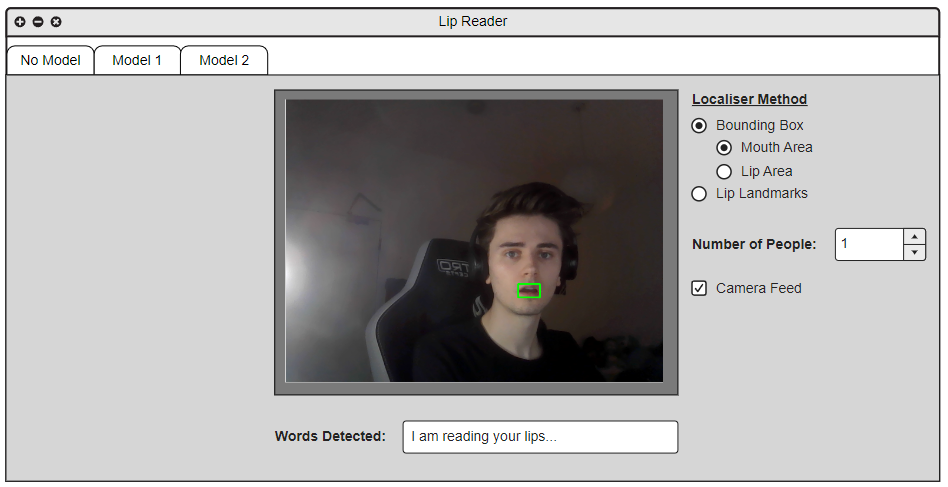
\includegraphics[width=0.5\textwidth]{GUI Mockup 1.png}}%
    % \qquad
    \subfloat[\centering Mockup iteration 2]{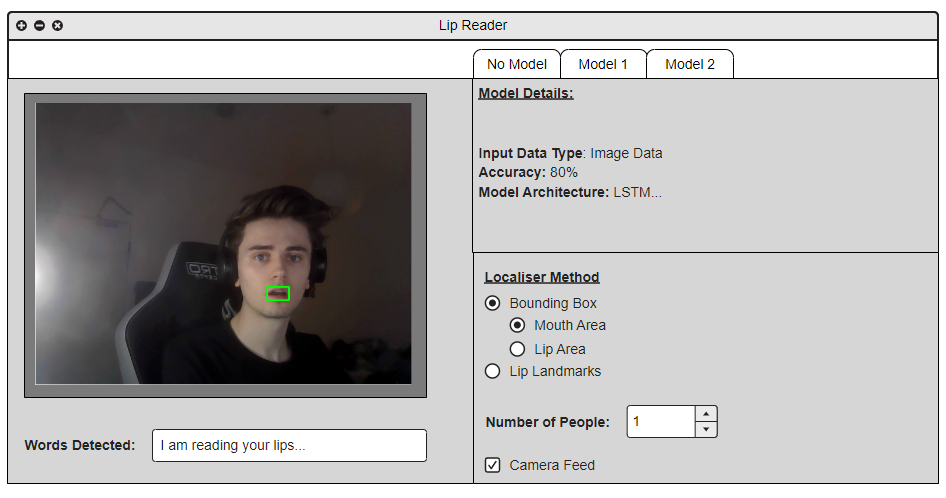
\includegraphics[width=0.5\textwidth]{GUI Mockup 2.png}}\\
    \subfloat[\centering Mockup iteration 3]{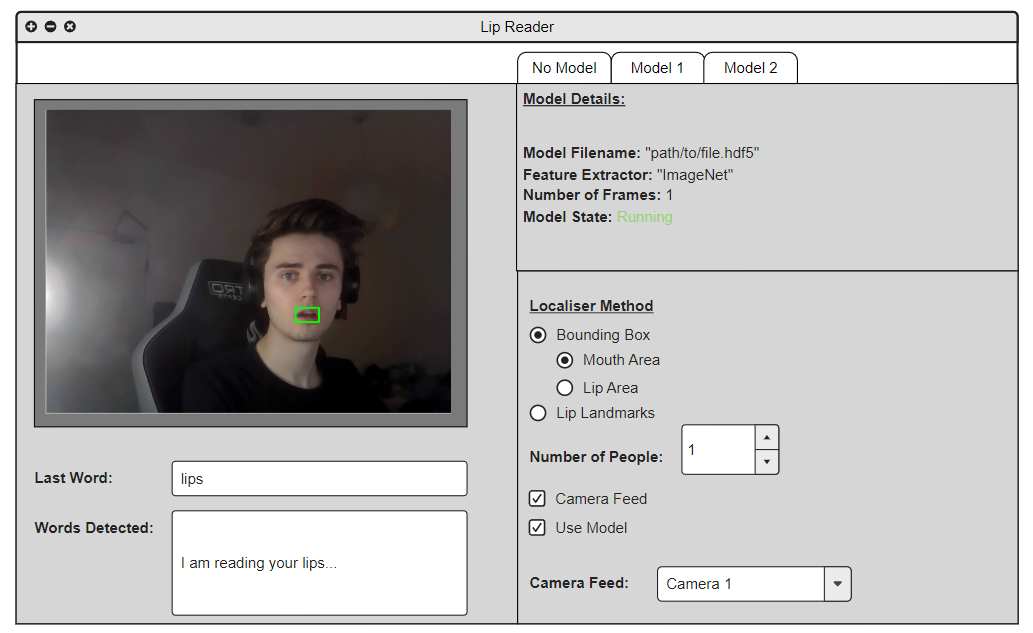
\includegraphics[width=0.5\textwidth]{GUI Mockup 3.png}}%
\caption[The three mockup iterations of the \acrfull{gui}]{The three mockup iterations of the \acrfull{gui}. The first stage included changing between models, realtime video feed and control over localisation. The second altered mainly the look of the system. The final mockup added further controls for the model, mainly in the inference methods, and more important model details.}
\label{fig:gui mockups}
\end{figure}
The design of the \acrshort{gui} went through three short iterations of mockups, as shown in Figure~\ref{fig:gui mockups}. All mockups were made using moqups\footnote{\url{https://moqups.com/}}. After these mockups were developed, the main \acrshort{gui} was produced using Tkinter. The remaining time within this project permitted the \acrshort{gui} to be extended, adding an extra tab within the window for model \gls{fine-tuning}. This is shown further in Figure~\ref{fig:annotated gui}.
\begin{figure}
\centering
    \subfloat[\centering Inference Tab]{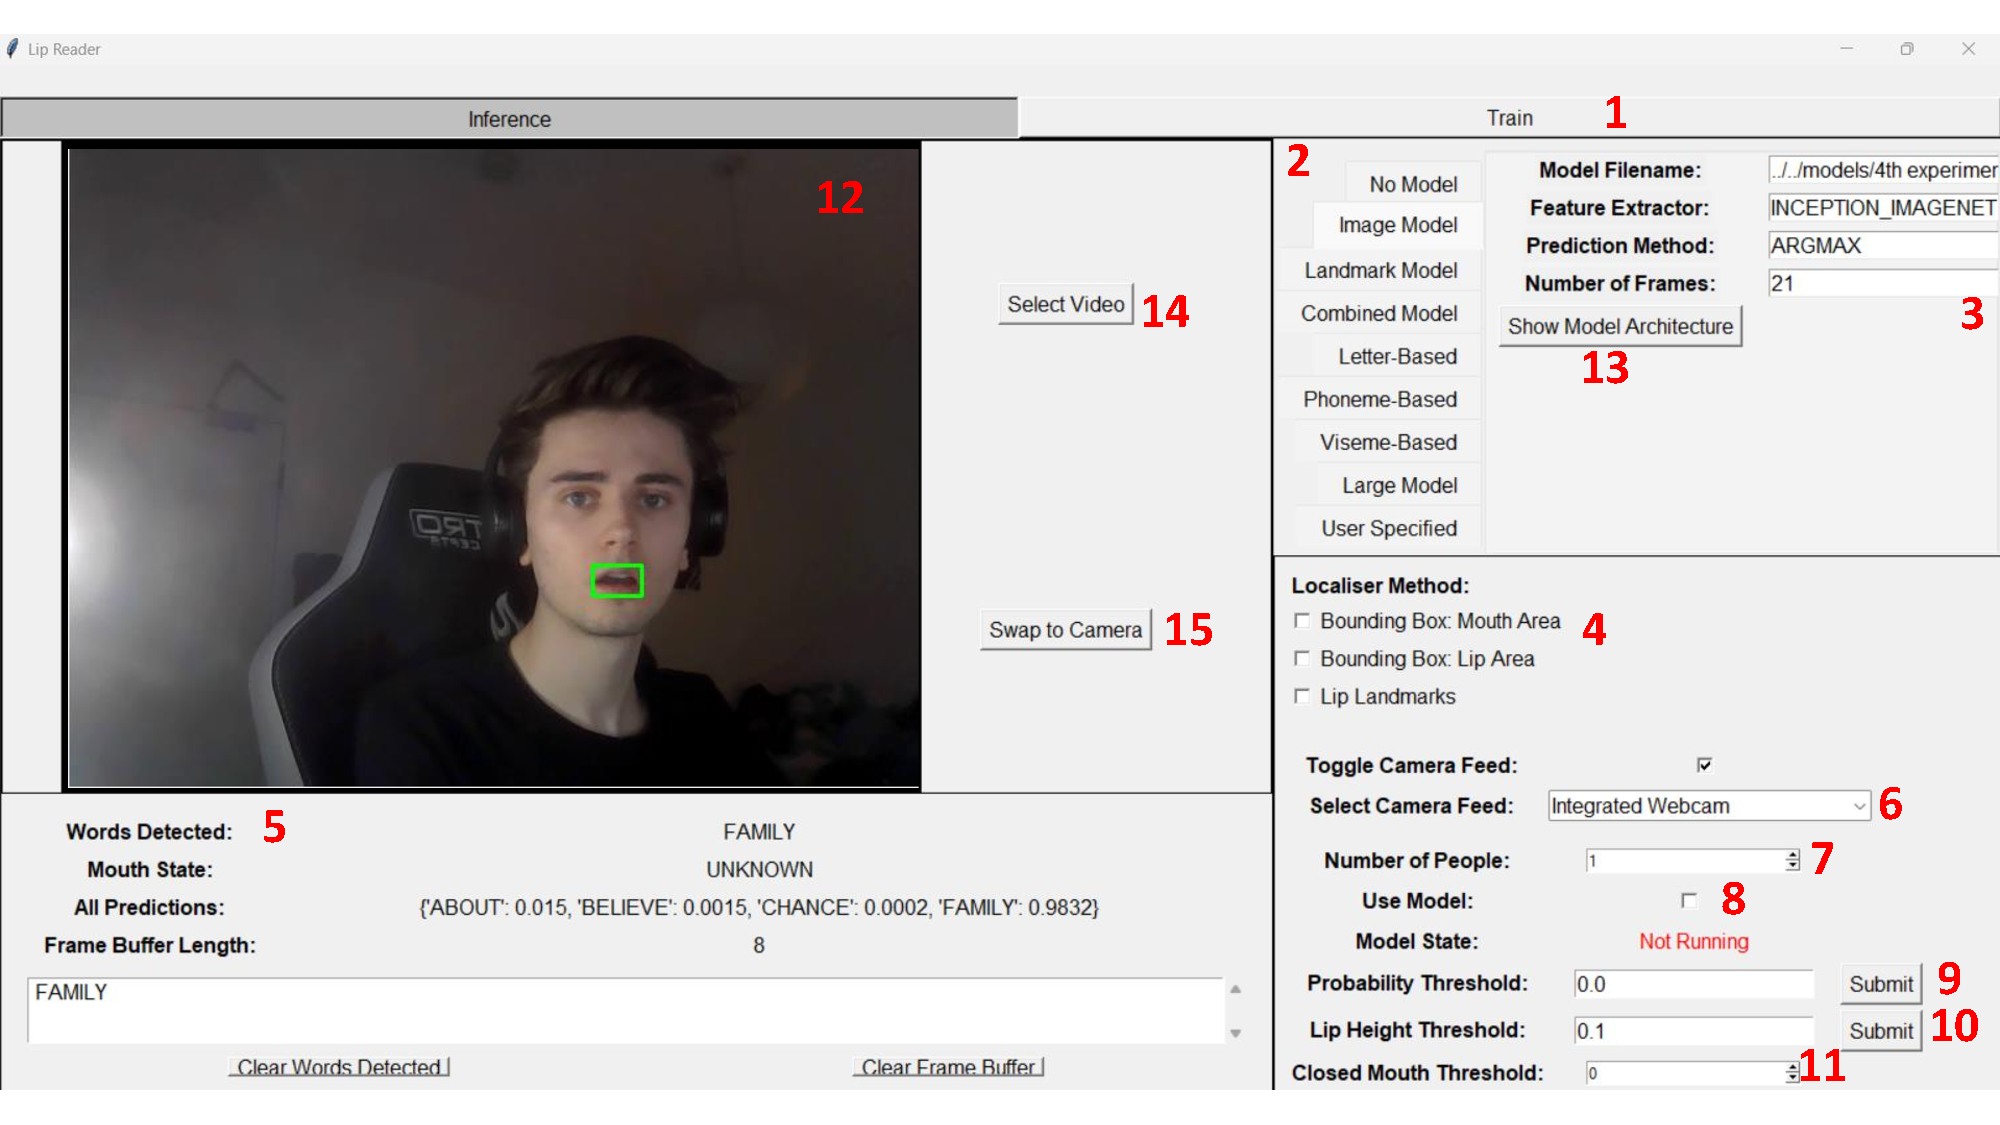
\includegraphics[width=0.5\textwidth]{Annotated GUI Inference.pdf}}
    \subfloat[\centering Training (\gls{fine-tuning}) Tab]{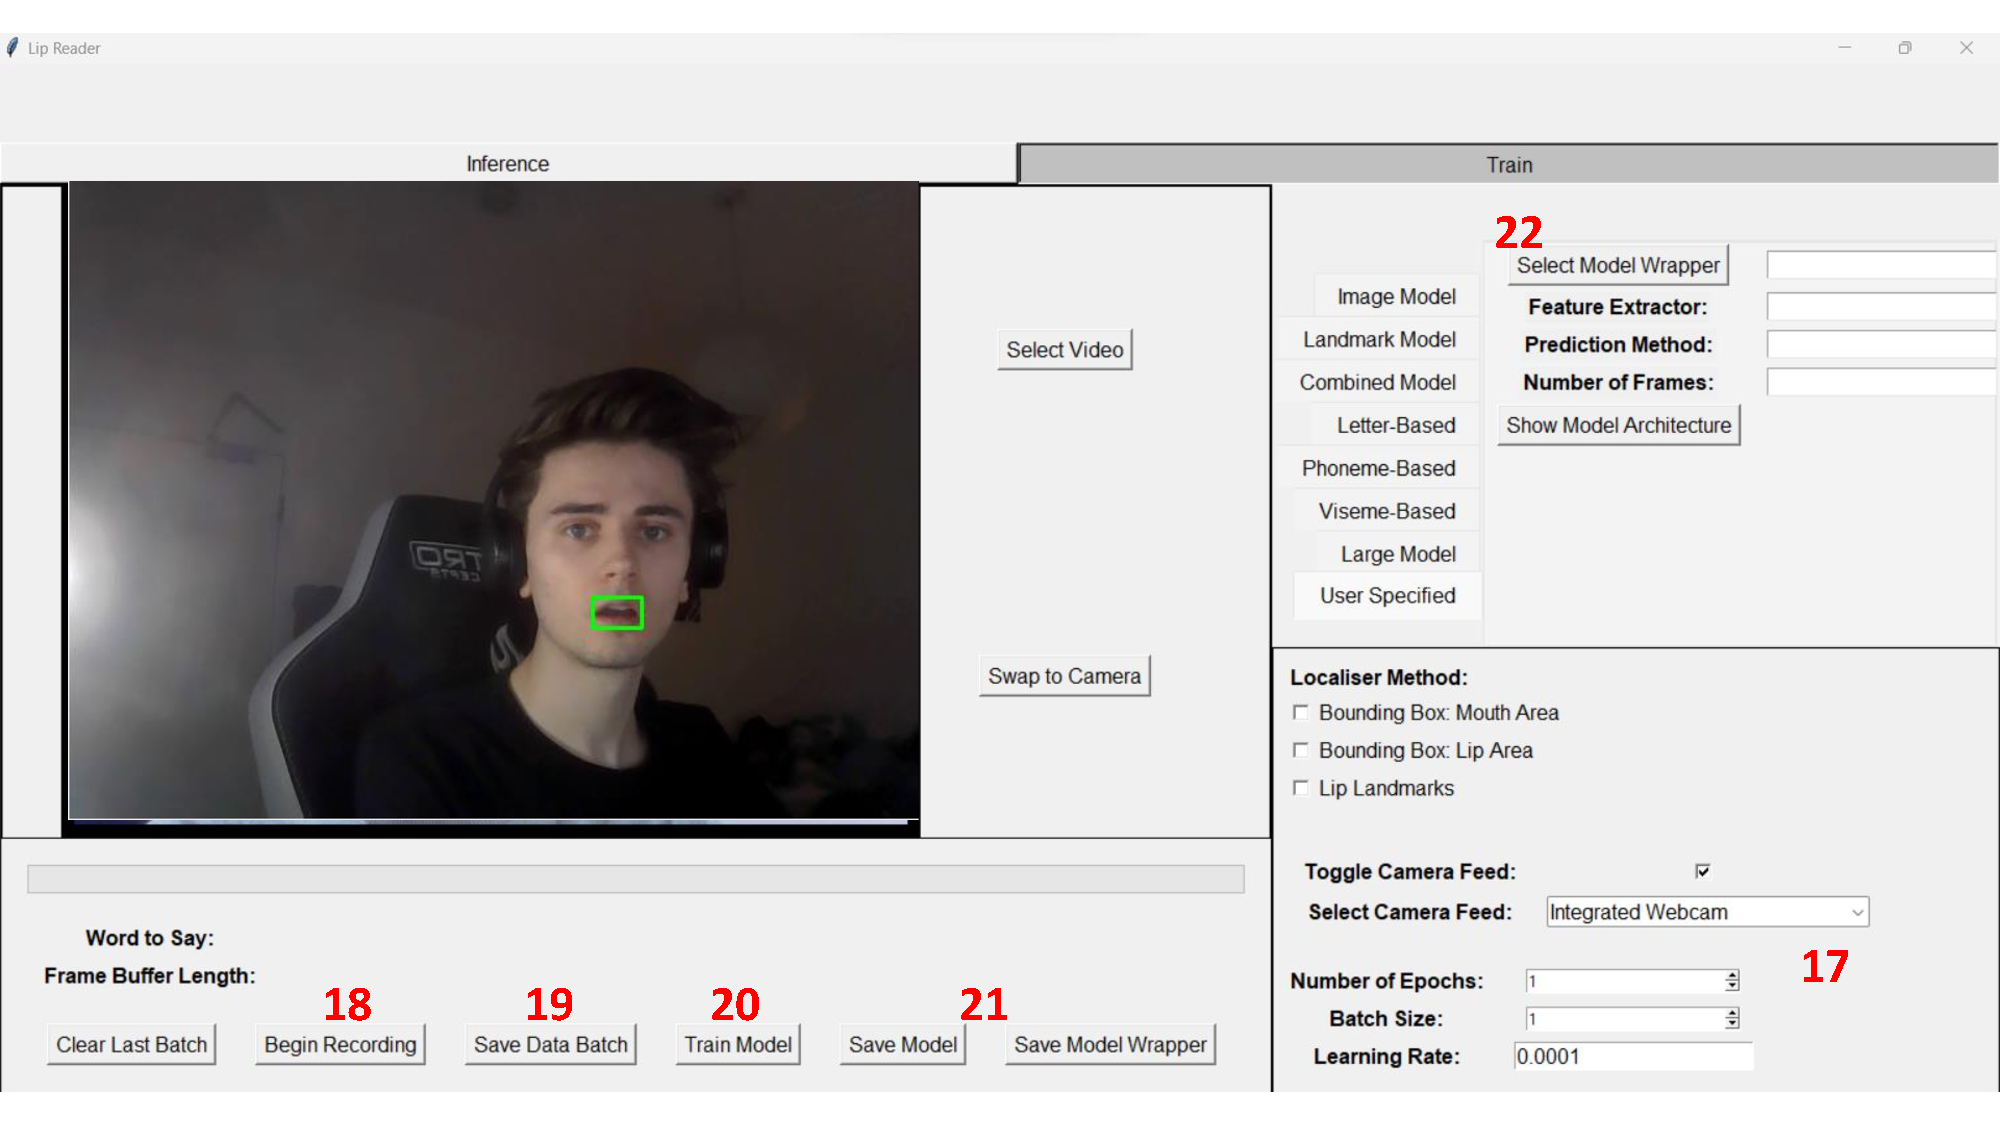
\includegraphics[width=0.5\textwidth]{Annotated GUI Train.pdf}}\\
\caption[The labelled \acrfull{gui}.]{The labelled \acrfull{gui}. This labels each of the primary features of the fully implemented \acrshort{gui}. Here both tabs for the \acrshort{gui} are shown: inference and training (or rather, \gls{fine-tuning}).}
\label{fig:annotated gui}
\end{figure}
The features of the \acrshort{gui} are presented below:
\begin{enumerate}
    \item \textbf{Mode Selector}: Used to change the interface between inference and training (or \gls{fine-tuning})
    \item \textbf{Model Selector}: Used to change between different trained models. Only a subset of the models are provided to select between. Note the change here that a vertical layout was employed rather than horizontal. This was to allow for better distinction between the different models
    \item \textbf{Model Properties}: This pane is used to give details about each of the different models
    \item \textbf{Localiser Method}: This configures display feed annotation, drawing bounding boxes around the lip or mouth area, or displaying the lip landmarks. This process is outlined more in Sections~\ref{sec: Visual Feature Extraction} and \ref{sec: Landmark Feature Extraction}
    \item \textbf{Prediction Frame}: This displays the current prediction, the past predictions and the frame buffer length (as it fills up). This displays the current mouth state (open or closed), the process for which is explained in Item~\ref{item: Lip Height Threshold} and Item~\ref{item: Closed Mouth Threshold}
    \item \textbf{Camera Feed Selection}: Python was used to detect all available cameras connected to the current device. These were then presented in a drop-down box for selection 
    \item \textbf{Number of People in Frame}: Used to configure MediaPipe to detect the correct number of people in the frame. Utilised to display bounding boxes for the lips of several people
    \item \textbf{Enable Model}: Used to begin running the model or pause it from making inference
    \item \textbf{Probability Threshold}: The threshold for prediction probabilities. Predictions below this predictions will be set to \textit{UNKNOWN}
    \item \textbf{Lip Height Threshold}: The threshold for the distance between the average of the upper landmarks and the average of the lower landmarks. Below this threshold the lips are considered to be together, and therefore closed, for the current frame \label{item: Lip Height Threshold}
    \item \textbf{Closed Mouth Threshold}: A threshold for the number of frames in a row that the mouth is closed for. If the number exceeds this value then predictions will stop being made as the lips are considered as being closed. This saves computation by having the model switch off for a person who isn't speaking. When set to 0 this feature is not used to stop predictions \label{item: Closed Mouth Threshold}
    \item \textbf{Display Area}: This displays the current feed of the selected camera
    \item \textbf{Model Architecture}: Clicking this button will open another window, displaying the model architecture of the currently selected model. This diagram is automatically generated in real-time using Keras util's plot\_model\footnote{\url{https://www.tensorflow.org/api_docs/python/tf/keras/utils/plot_model}} function
    \item \textbf{Select Video}: This creates a file dialogue box, allowing selection of a video file. This file will then be repeatedly played in the window and used for inference
    \item \textbf{Swap to Camera}: This swaps the feed back to the currently selected input stream
    \item \textbf{\Gls{fine-tuning} Configuration}: This area is used to modify and control the settings for model \gls{fine-tuning} such as the \acrshort{lr}, epochs and batch size \label{item: fine-tune settings}
    \item \textbf{Begin Recording}: Activates data collection, starting to collect frames from the input stream for the current word \label{item: begin recording} 
    \item \textbf{Save Data Batch}: This will temporarily save the data sample to be used for \gls{fine-tuning} later \label{item: save data} 
    \item \textbf{Train Model}: This model starts \gls{fine-tuning} of the model using the data \label{item: finetune} 
    \item \textbf{Model Saving}: These buttons are used to save the currently selected model or whole model wrapper to be loaded in and used through Item~\ref{item: load model}
    \item \textbf{Load Model}: Selecting the ``User Specified" model shows this feature. Clicking this button creates a dialogue, allowing a model wrapper file to be found and selected for use \label{item: load model} 
\end{enumerate}
One of the main, complex features of the \acrshort{gui} is that of stopping inference when the mouth is closed. This is controlled using Items~\ref{item: Closed Mouth Threshold} and \ref{item: Lip Height Threshold}. Item~\ref{item: Closed Mouth Threshold} controls the relative height between the upper and low lips. When this height is less than the threshold, the lips are considered closed. Item~\ref{item: Lip Height Threshold} controls inference associated with when the user has stopped speaking, stopping the model from predicting if it considers the speaker to have paused for a time.\\
Another feature worth further explanation is that of \gls{fine-tuning} lip reading models. To fine-tune the model, a user is presented with the classes of the currently selected model. They can select Item~\ref{item: begin recording} to begin recording data for \gls{fine-tuning} and Item~\ref{item: save data} to save that data internally. When Item~\ref{item: finetune} is selected \gls{fine-tuning} of the current model will begin. This will utilise the training settings configured within Item~\ref{item: fine-tune settings} to fine-tune the current model. This could take some time depending on the settings. The resulting model metrics will be printed to the interface and the user can then opt to save the new model using Item~\ref{item: save data}. %Chapter 3
%   Design: ~ 30%: 4500 words
        % Current: 5246 words
\chapter{Experimentation and Results}
\label{cha:results}
\graphicspath{ {./experiments/} }
This chapter presents various model architectures and their performance on lip reading. It contrasts them and explains the workflow to develop the best possible lip reading model.
A summary of the experiments that will be performed is presented in Table~\ref{table: experiment summary}.
\begin{table}[h]
\centering
\begin{tabular}{|c|p{100mm}|} 
 \hline
 Experiment & Description\\
 \hline
 1 & A basic \acrshort{cnn} architecture feeding into an \acrshort{lstm} was trialled. Visual features were used as input\\
 2 & Data augmentation and frame pruning were utilised during pre-processing\\ 
 3 & A pure \acrshort{bilstm} architecture was swapped in and assessed\\
 4 & Manual \acrshort{lr} scheduling was explored. Sub-experiments explored different hyperparameter settings\\
 5 & Landmark features were used as input to the model\\
 6 & Further methods for data augmentation were employed to reduce \gls{overfitting}\\
 7 & A \gls{transformer} architecture was trialled \\
 8 & A combination of landmark and visual features were used as input to the model\\
 \hline
 9 & Letters, \gls{phoneme}s and \gls{viseme}s were assessed, respectively, to find the best classes for lip reading \\
 \hline
\end{tabular}
\caption[A brief summary and description of the different experiments]{A brief summary and description of the different experiments. Note that a line divides the final three experiments due to a different loss, \acrshort{ctc} loss, being utilised.}
\label{table: experiment summary}
\end{table}
\section{Experiment 1: Base Architecture}
\label{sec: Experiment 1}
% Experiment 2
% Basic architecture. CNN followed by lstm
\subsection{Model Architecture}
\begin{figure}
\centering
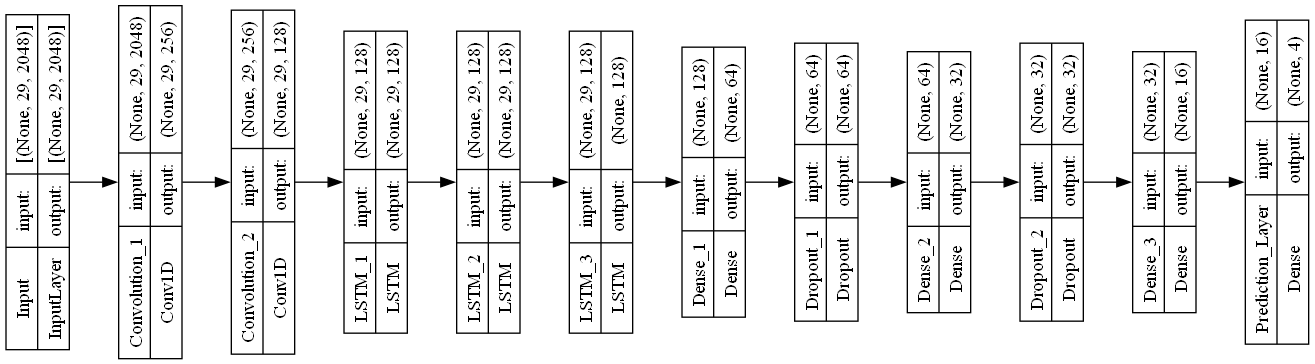
\includegraphics[width=0.9\textwidth]{model architectures/1 architecture.png}
\caption[Experiment 1 architecture]{Experiment 1 architecture. This depicts two 1D convolution layers, followed by three \acrshort{lstm} layers and then a set of dense layers with some dropout. The ``None" above refers to the batch size. Models are trained with batches of data which contain several samples of data. The 29 refers to the number of frames expected by the model. The final number for each layer is that layer's size.}
\label{fig:1 architecture}
\end{figure}
The first experiment used a basic model architecture as a basis to improve upon. The model architecture used, as shown in Figure~\ref{fig:1 architecture}, began with an input layer\footnote{\url{https://www.tensorflow.org/api_docs/python/tf/keras/layers/InputLayer}} to automatically configure the input shape accepted by the model. Two 1D convolutional\footnote{\url{https://keras.io/api/layers/convolution_layers/}} and three unidirectional \acrshort{lstm} layers\footnote{\url{https://keras.io/api/layers/recurrent_layers/lstm/}} followed this. Finally a series of dense\footnote{\url{https://keras.io/api/layers/core_layers/dense/}} and dropout layers\footnote{\url{https://keras.io/api/layers/regularization_layers/dropout/}} were employed before a prediction layer output the probabilities of the input sample belonging to each of the different classes within the dataset.\\
This architecture was inspired by Chung et al.~\cite{Lip-Reading-In-The-Wild} who suggested extending their architecture of \acrshort{cnn} to additionally include \acrshort{lstm} units.\\
1D convolution was used here as the input data only consisted of image feature vectors of the size (1, 2048). ReLU activation functions were used for each layer, excluding the final prediction layer which instead employed Softmax.\\
\Gls{dropout} layers were employed as a means of regularisation~\cite{regularization_for_DL, dropout_for_overfitting}, to avoid \gls{overfitting}. A value of 0.2 was used to drop 20\% of input units during training.\\
Categorical cross-entropy loss was used to train the model, outlined in Section~\ref{sec: Cross-Entropy Loss}. The classes used were the \gls{one_hot_encoding}s for the four word classes: \emph{about}, \emph{believe}, \emph{chance} and \emph{family}.\\
The model was trained for 100 epochs to allow for sufficient time for the model to capture nuances within the training data whilst maintaining a shorter training time. A batch size of 32 was used for similar reasons.\\
Finally, the Adam optimiser alone was used with a \acrshort{lr} of $1\times10^{-5}$. A very small \acrshort{lr} was used because lip reading is a very nuanced and subtle process.
\subsection{Results and Evaluation}
\begin{figure}
\centering
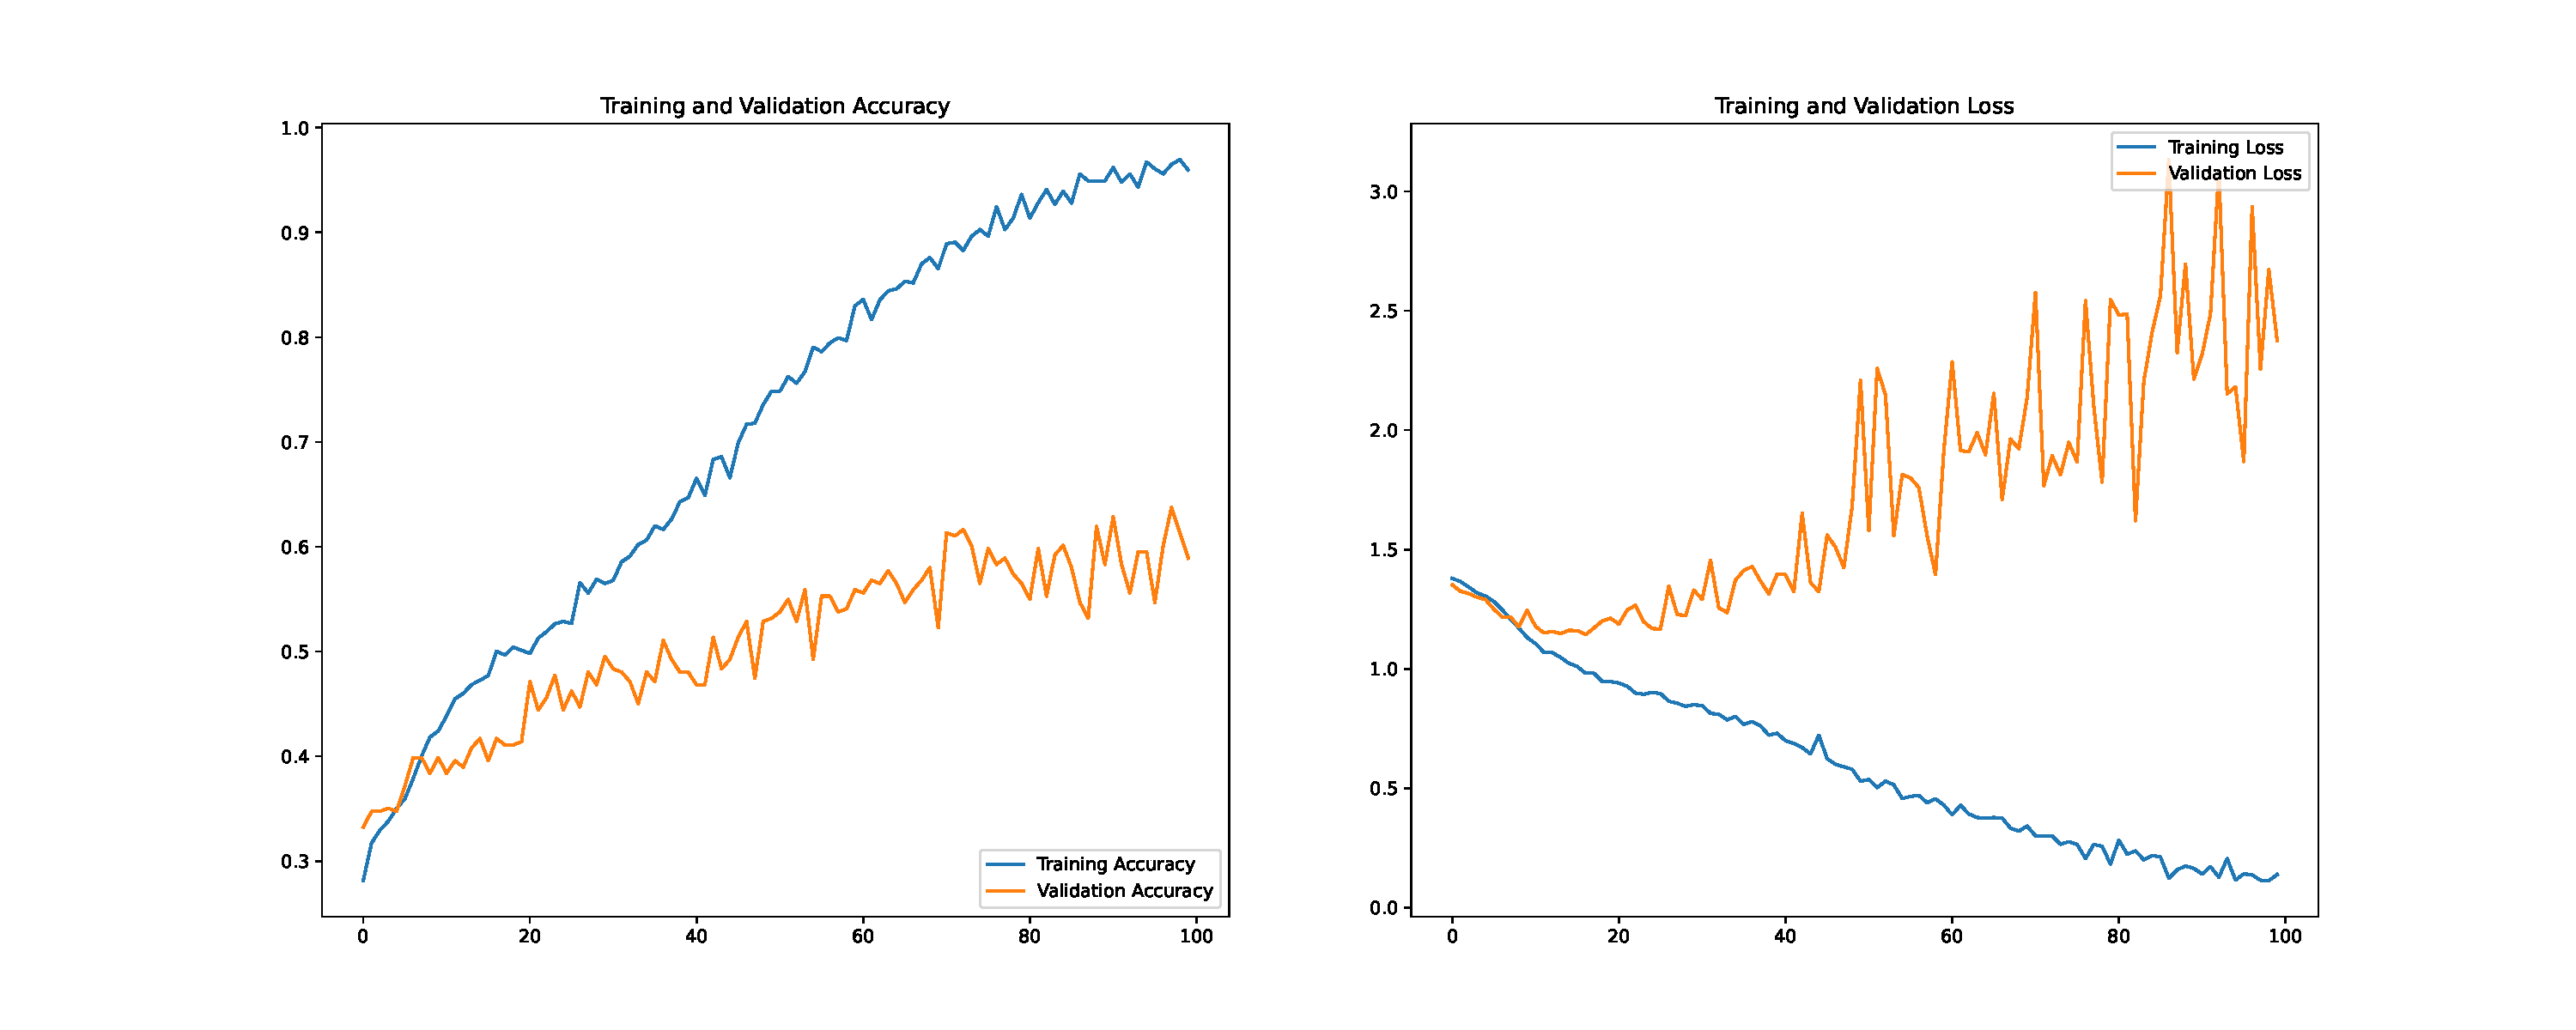
\includegraphics[width=1\textwidth]{metrics/1 metrics.pdf}
\caption[Experiment 1 results]{Experiment 1 results. This depicts training and testing accuracy and loss. Accuracy measures of the number of videos that were given the correct label of the word being spoken. Loss gives a measure of the categorical cross-entropy loss of the different predictions.}
\label{fig:1 results}
\end{figure}
\begin{table}
\centering
\begin{tabular}{|c|c|c|c|} 
 \hline
 Experiment &  Testing Accuracy & Testing Loss & \acrshort{wer} \\ [0.2ex] 
 \hline
 1 & \accuracyone & \lossone & \werone \\ 
 \hline
\end{tabular}
\caption[The testing accuracy, loss and \acrshort{wer} for experiment 1]{The testing accuracy, loss and \acrshort{wer} for experiment 1. These results were captured by running the model against a testing dataset: a dataset that was not used during training of the model.}
\label{table: 1 results}
\end{table}
The first experiment yielded promising results, as shown in Figure~\ref{fig:1 results} and Table~\ref{table: 1 results}. Clear \gls{overfitting} occurred early within training, evident by the training and testing accuracies and losses diverging early. There could be many potential causes of \gls{overfitting} such as there not being enough data, data being too noisy or the model being too complex. There are many potential ways to reduce \gls{overfitting}. These include \gls{data_augmentation}, data regularisation~\cite{regularization_for_DL, dropout_for_overfitting} or reducing the size and complexity of the model.\\
Due to the results of this experiment, the second experiment instead employed some \gls{data_augmentation} methods,  attempting to reduce noise within the data.
\section{Experiment 2: Frame Pruning}
\label{sec: Experiment 2}
% Experiment 3
% Added frame pruning & data_augmentation
\subsection{Model Architecture}
The same model architecture was used as in Section~\ref{sec: Experiment 1}. However, further data preprocessing was carried out before training, aiming to reduce \gls{overfitting}.\\
As outlined within Section~\ref{sec: LRW Dataset}, the structure of \gls{lrw} are 29 frame videos that contain multiple word utterances. Only the primary word utterances (\emph{about}, \emph{believe}, \emph{chance} or \emph{family}) within each video are labelled. Whilst this can be beneficial, this could result in \gls{overfitting}. This is because the model might fixate on commonly occurring words around the primary word, such as ``I believe" rather than ``believe". This could cause \gls{underfitting} if the data samples are too noisy, resulting in difficulty converging to a valid solution.\\
This experiment employed two methods to overcome \gls{overfitting} encountered within Section~\ref{sec: Experiment 1}: frame pruning and \gls{data_augmentation}.\\
Frame pruning was used to remove frames from the start and end of video data samples, focusing more on the central part of the video and thus the primary word utterance. This could reduce \gls{overfitting} as there is less noise present in the data.\\
The downside of frame pruning is that it could introduce \gls{underfitting} or worsen the performance of models. Indiscriminate removal of frames could remove intrinsic information from each data sample.\\
The method used for \gls{data_augmentation} was horizontal flipping. The frames for each video were horizontally flipped, and these new samples were added to the dataset. This had the effect of doubling the amount of data available for training, validation and testing. This method was used as it is one of the easiest \gls{data_augmentation} methods to implement~\cite{og_data_augmentation} whilst still creating diverse enough data.\\
The downside of this \gls{data_augmentation} method is that it could lead to \gls{overfitting}. After \gls{data_augmentation} there will be two copies of every \gls{lrw} sentence, possibly worsening the issue of noisy words. If the model has even more samples of ``I believe" it may become even more focused on the noisy ``I", regardless of frame flipping. This data augmentation method will preserve the structure of sentences; whilst the data might visually be different, it is not semantically diverse\\
Only 50 epochs were carried out for this training run, to conserve computational power. \Gls{overfitting} occurred early within the first training run and thus a high epoch number was not required to observe a similar result.
\subsection{Results and Evaluation}
\begin{figure}
\centering
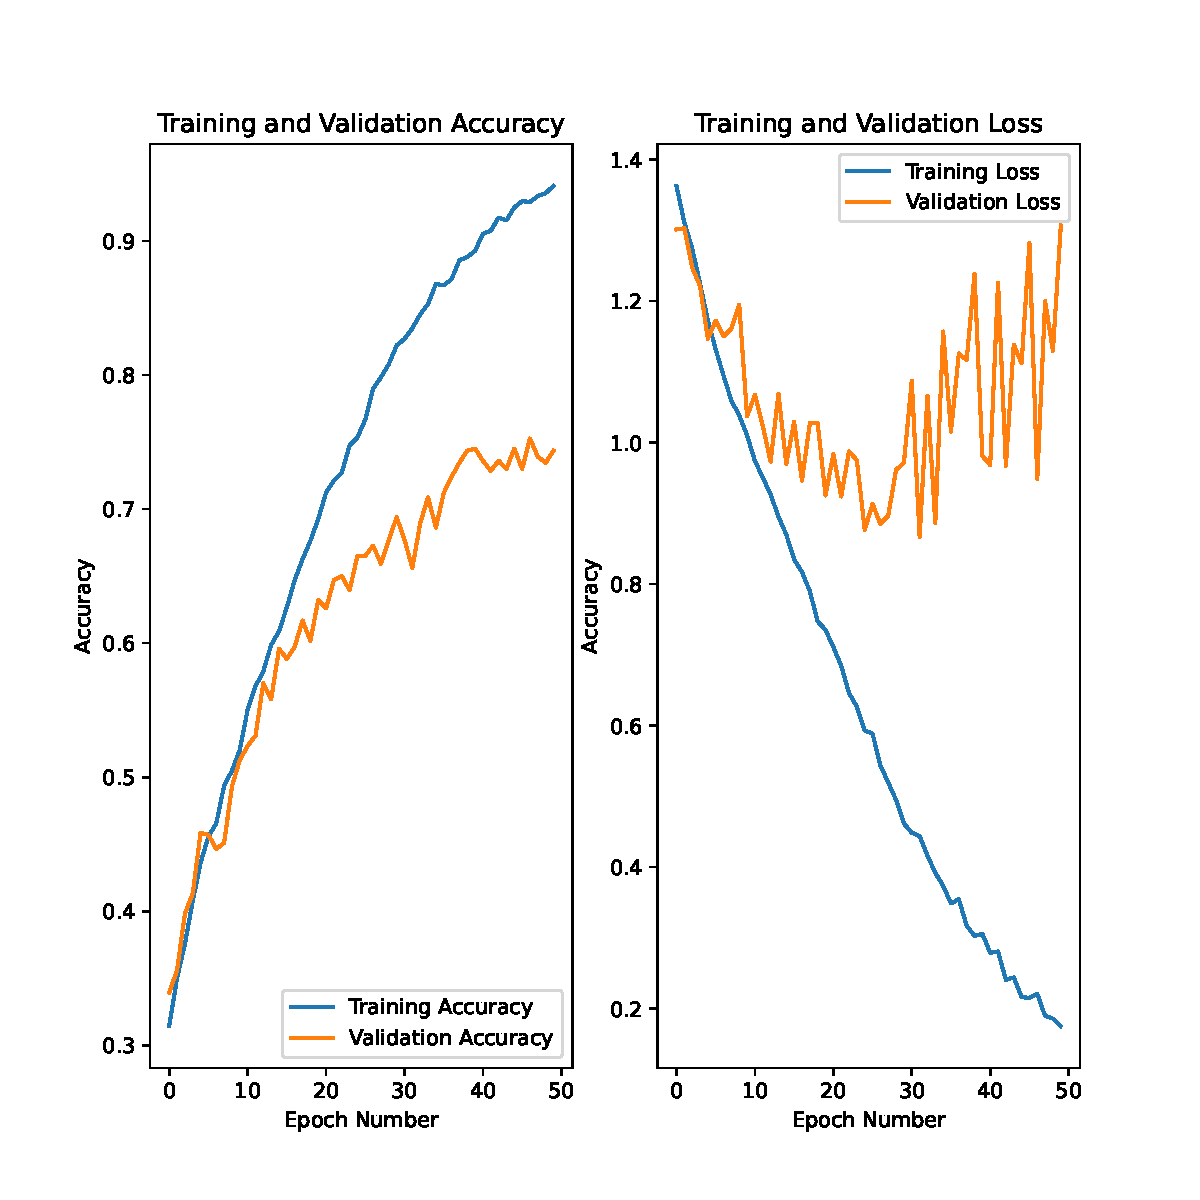
\includegraphics[width=0.5\textwidth]{metrics/2 metrics.pdf}
\caption[Experiment 2 results]{Experiment 2 results. This shows the effect of adding frame pruning and \gls{data_augmentation}.}
\label{fig:2 results}
\end{figure}
\begin{table}
\centering
\begin{tabular}{|c|c|c|c|} 
 \hline
 Experiment &  Testing Accuracy & Testing Loss & \acrshort{wer} \\ [0.2ex] 
 \hline
 2 & \accuracytwo & \losstwo & \wertwo \\ 
 \hline
\end{tabular}
\caption{The testing accuracy, loss and \acrshort{wer} for experiment 2.}
\label{table: 2 results}
\end{table}
As shown in Figure~\ref{fig:2 results} and Table~\ref{table: 2 results}, this model performed better than the previous experiment. Early stopping helped to reduce the effect of \gls{overfitting} and improve the accuracy of the model.\\
In conclusion, frame pruning and \gls{data_augmentation} did benefit the process; however, \gls{overfitting} was still occurring.
\section{Experiment 3: Bidirectional LSTM Architecture}
\label{sec: Experiment 3}
% Experiment 7
% Bi-lstm
\subsection{Model Architecture}
\begin{figure}
\centering
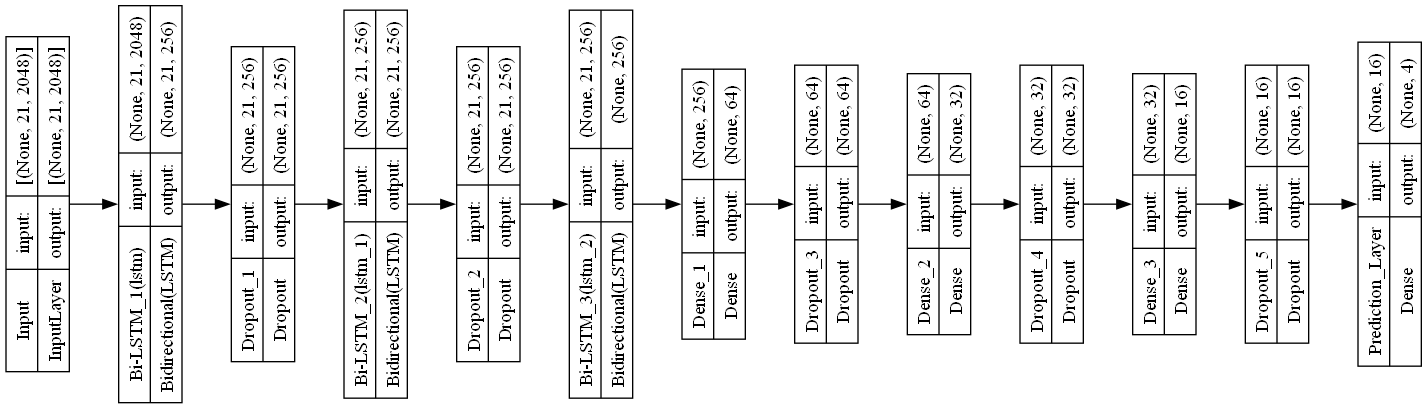
\includegraphics[width=0.9\textwidth]{model architectures/3 architecture.png}
\caption[Experiment 3 architecture]{Experiment 3 architecture. This depicts the \acrshort{bilstm} architecture employed for lip reading. The model took visual feature vectors as input to a series of \acrshort{bilstm} layers. \Gls{dropout} was employed after each layer to reduce the effect of \gls{overfitting}. ReLU activation functions were utilised for each layer except the final which employed Softmax.}
\label{fig:3 architecture}
\end{figure}
For this experiment, a different model architecture was investigated (see Figure~\ref{fig:3 architecture}). Rather than a \acrshort{cnn} combined with an \acrshort{lstm}, a pure \acrshort{bilstm}\footnote{\url{https://keras.io/api/layers/recurrent_layers/bidirectional/}} architecture was studied.\\
Typically, convolution is utilised for image or video data (2D or 3D data) to reduce the dimensionality of the data and looking at the relationship between image regions. However, for this experiment we have already employed a visual feature extractor, effectively skipping this step.\\
In the previous experiment, only unidirectional \acrshort{lstm} layers were utilised. Instead in this experiment, we employed \acrshort{bilstm} layers to capture both left and right context within the videos.\\
Training lasted for 150 epochs, allowing the model more time to train and learn the data since a simple model was being investigated. Otherwise, the details of this experiment (\acrshort{lr}, early stopping, loss, etc) remained the same as the previous one. The same activation functions of ReLU were employed within the \acrshort{bilstm} layers.
\subsection{Results and Evaluation}
\begin{figure}
\centering
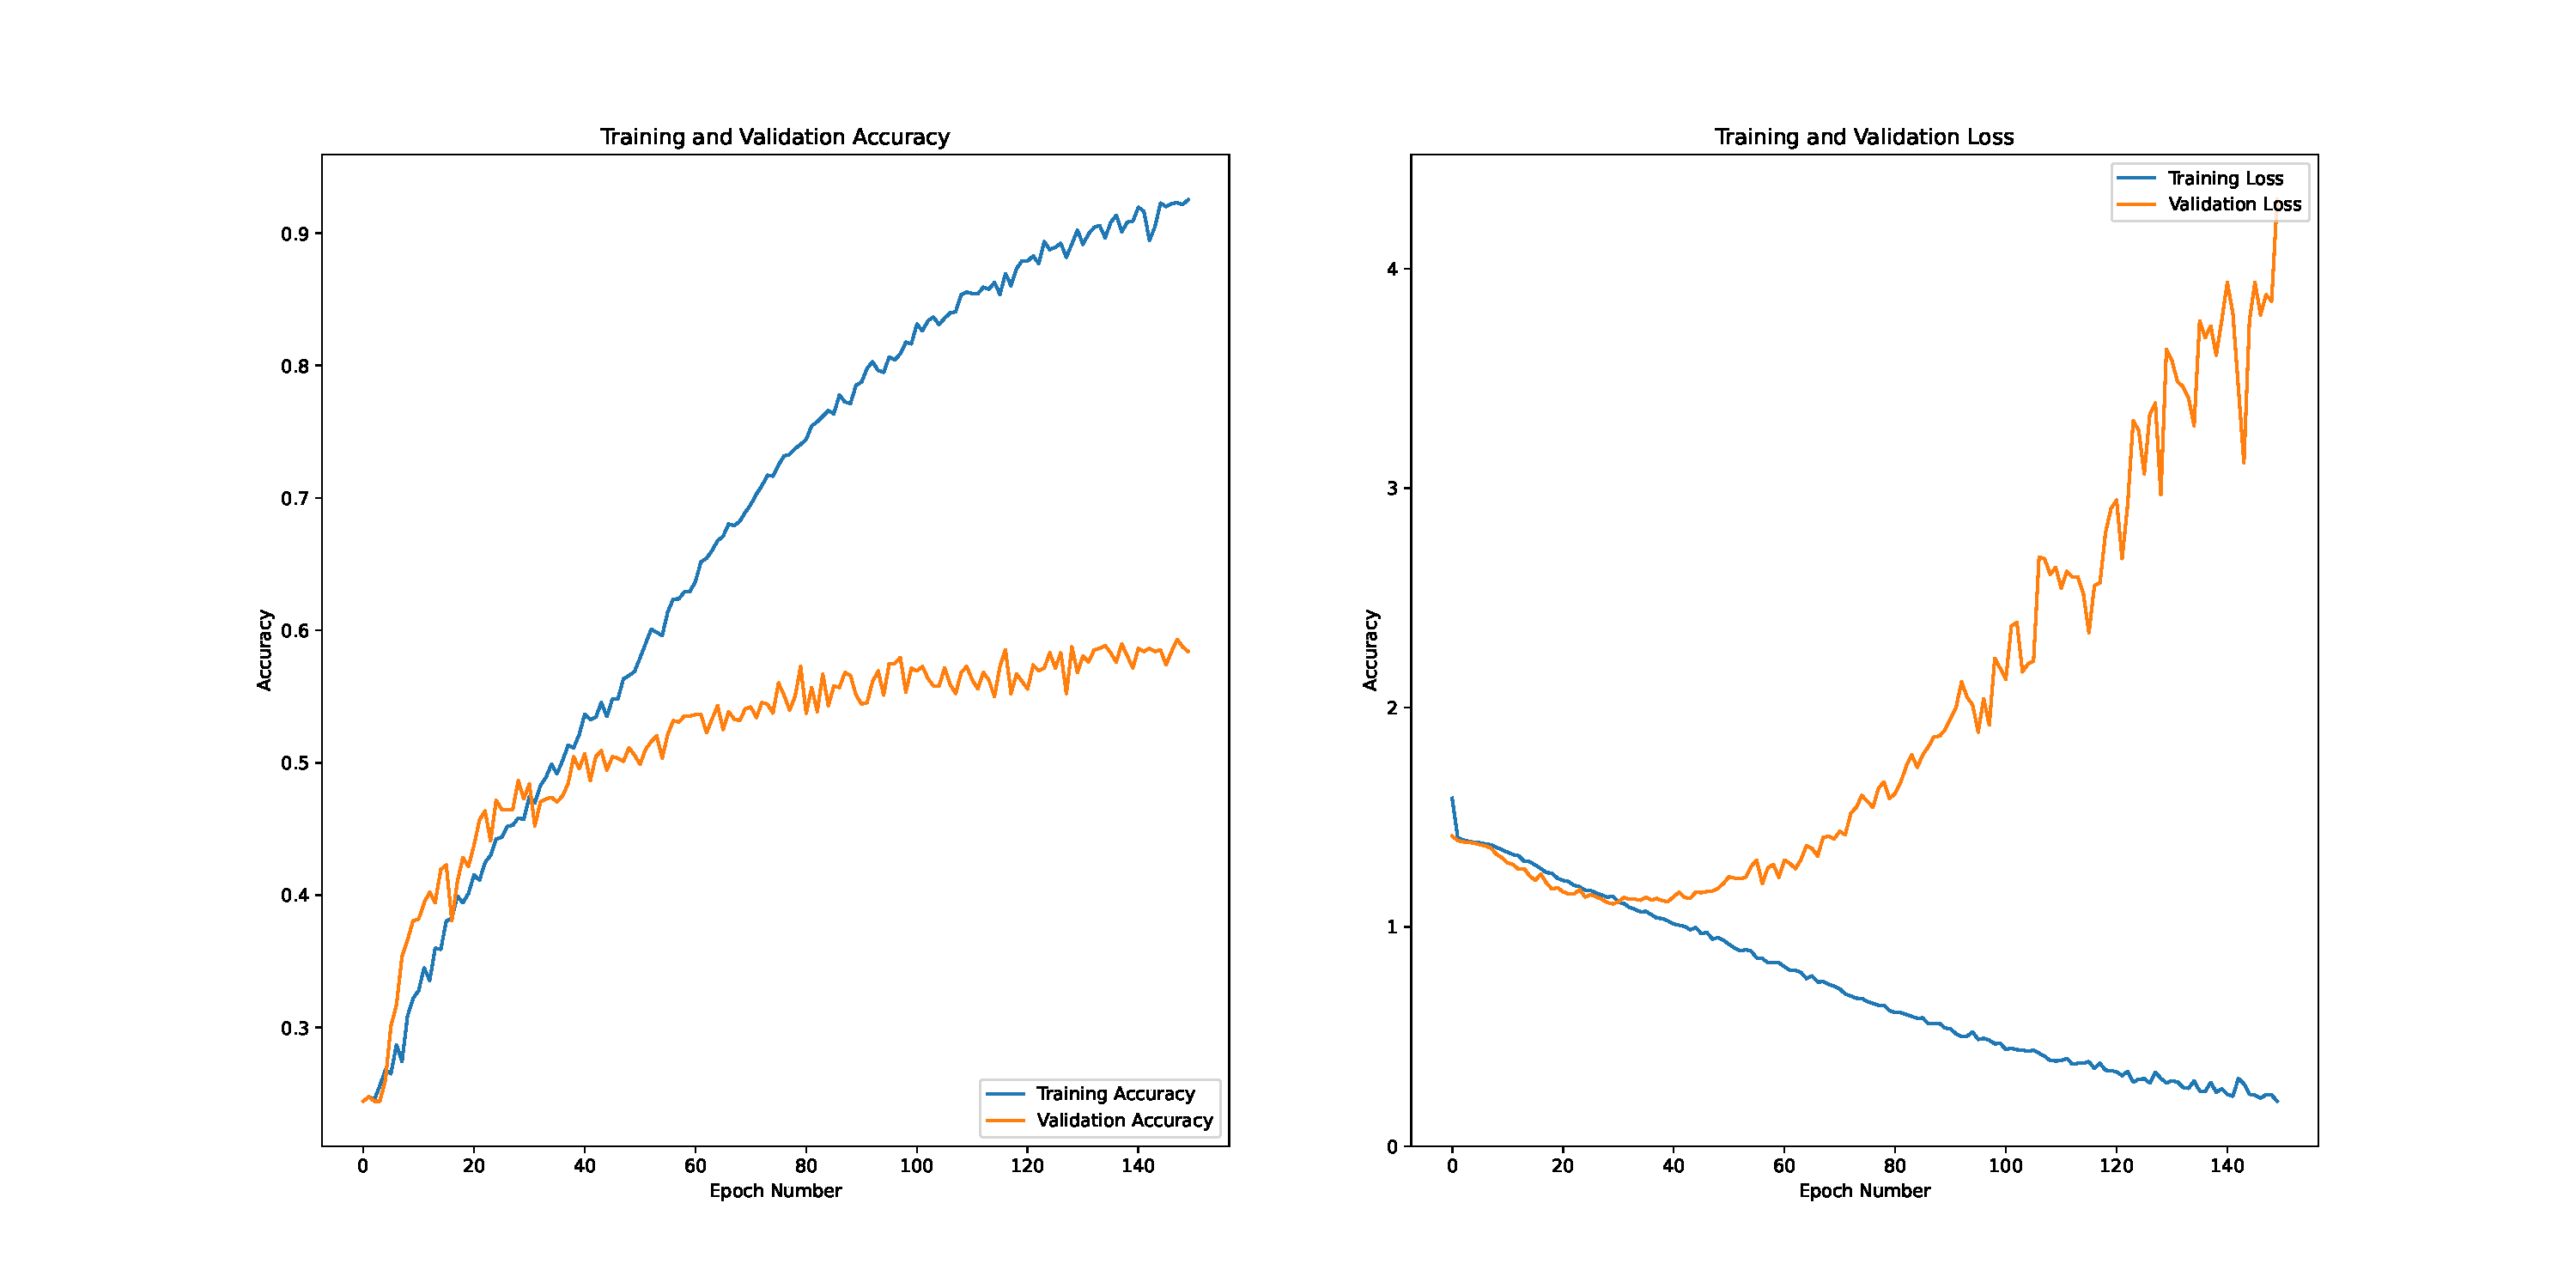
\includegraphics[width=1\textwidth]{metrics/3 metrics.pdf}
\caption[Experiment 3 results]{Experiment 3 results.}
\label{fig:3 results}
\end{figure}
\begin{table}
\centering
\begin{tabular}{|c|c|c|c|} 
 \hline
 Experiment &  Testing Accuracy & Testing Loss & \acrshort{wer} \\ [0.2ex] 
 \hline
 3 & \accuracythree & \lossthree & \werthree \\ 
 \hline
\end{tabular}
\caption{The testing accuracy, loss and \acrshort{wer} for experiment 3.}
\label{table: 3 results}
\end{table}
As shown in Figure~\ref{fig:3 results} and Table~\ref{table: 3 results}, this architecture actually performed worse than the previous models.\\
The maximum accuracy and minimum loss achieved were both lower than the models trained in the first and second experiments. However, \gls{overfitting} occurred later in training, giving promising results for this architecture.\\
Further experimentation was conducted on this architecture aiming to produce better results.
\section{Experiment 4: Manual Adaptive Learning Rate}
\label{sec: Experiment 4}
% Experiment 8
% Adaptive learning rate
\subsection{Model Architecture}
For this experiment, the same model architecture was used as in Section~\ref{sec: Experiment 3}; however, the \acrshort{lr} was changed.\\
Previously the Adam optimiser on its own had been employed to varying success. Instead, as mentioned in Section~\ref{sec: Learning Rate}, a combination of both the Adam optimiser and another \acrshort{lr} scheduling method is beneficial and thus was applied. For this experiment, Adam was used to control the \acrshort{lr} of parameters more precisely but the \acrshort{lr} was also altered manually.\\
Three primary experiments were carried out. In each, after 20 epochs the \acrshort{lr} was multiplied by a decimal value. The values used for the experiments were 0.9, 0.5 and 0.7.\\
A higher initial \acrshort{lr} of $1\times10^{-4}$ was used, compared with previous experiments. In most cases, a larger \acrshort{lr} should be used initially, decreasing this over time~\cite{batch-size-on-the-generalizability}. A large initial \acrshort{lr} allows the model to find the global minimum in the loss and then converge quickly as the \acrshort{lr} decreases.
\subsection{Results and Evaluation}
\begin{figure}
\centering
    \subfloat[\centering Experiment 4.1. \acrshort{lr} multiplier equals 0.9.]{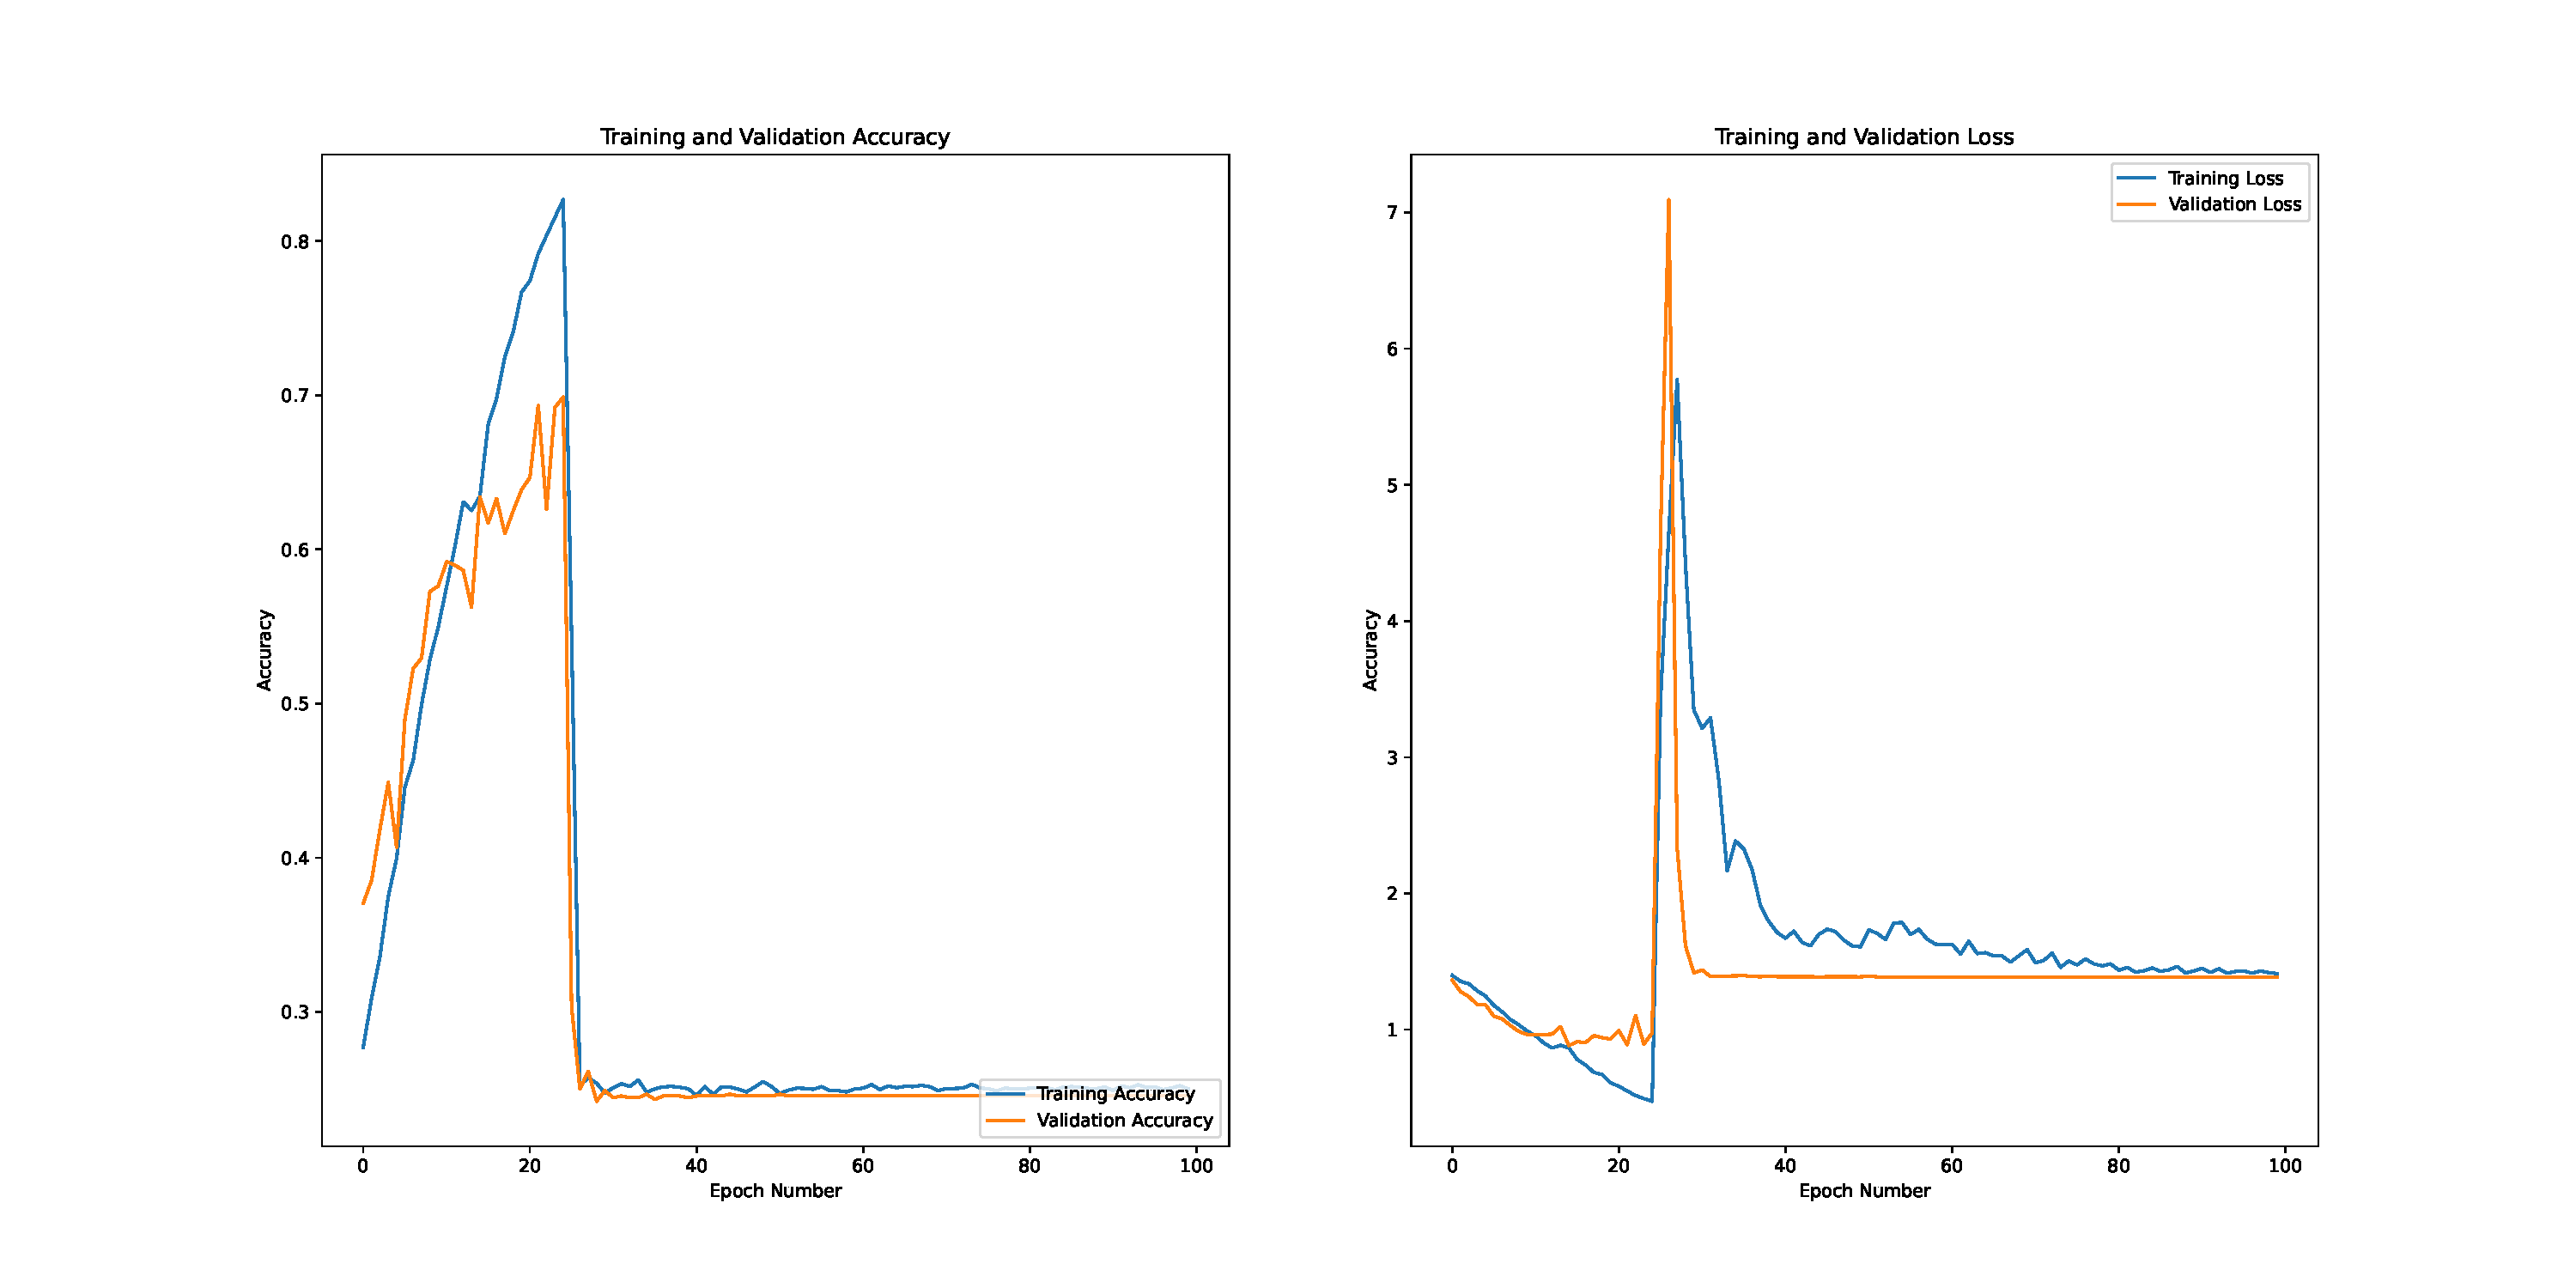
\includegraphics[width=0.5\textwidth]{metrics/4.1 metrics.pdf}}
    \subfloat[\centering Experiment 4.2. \acrshort{lr} multiplier equals 0.5.]{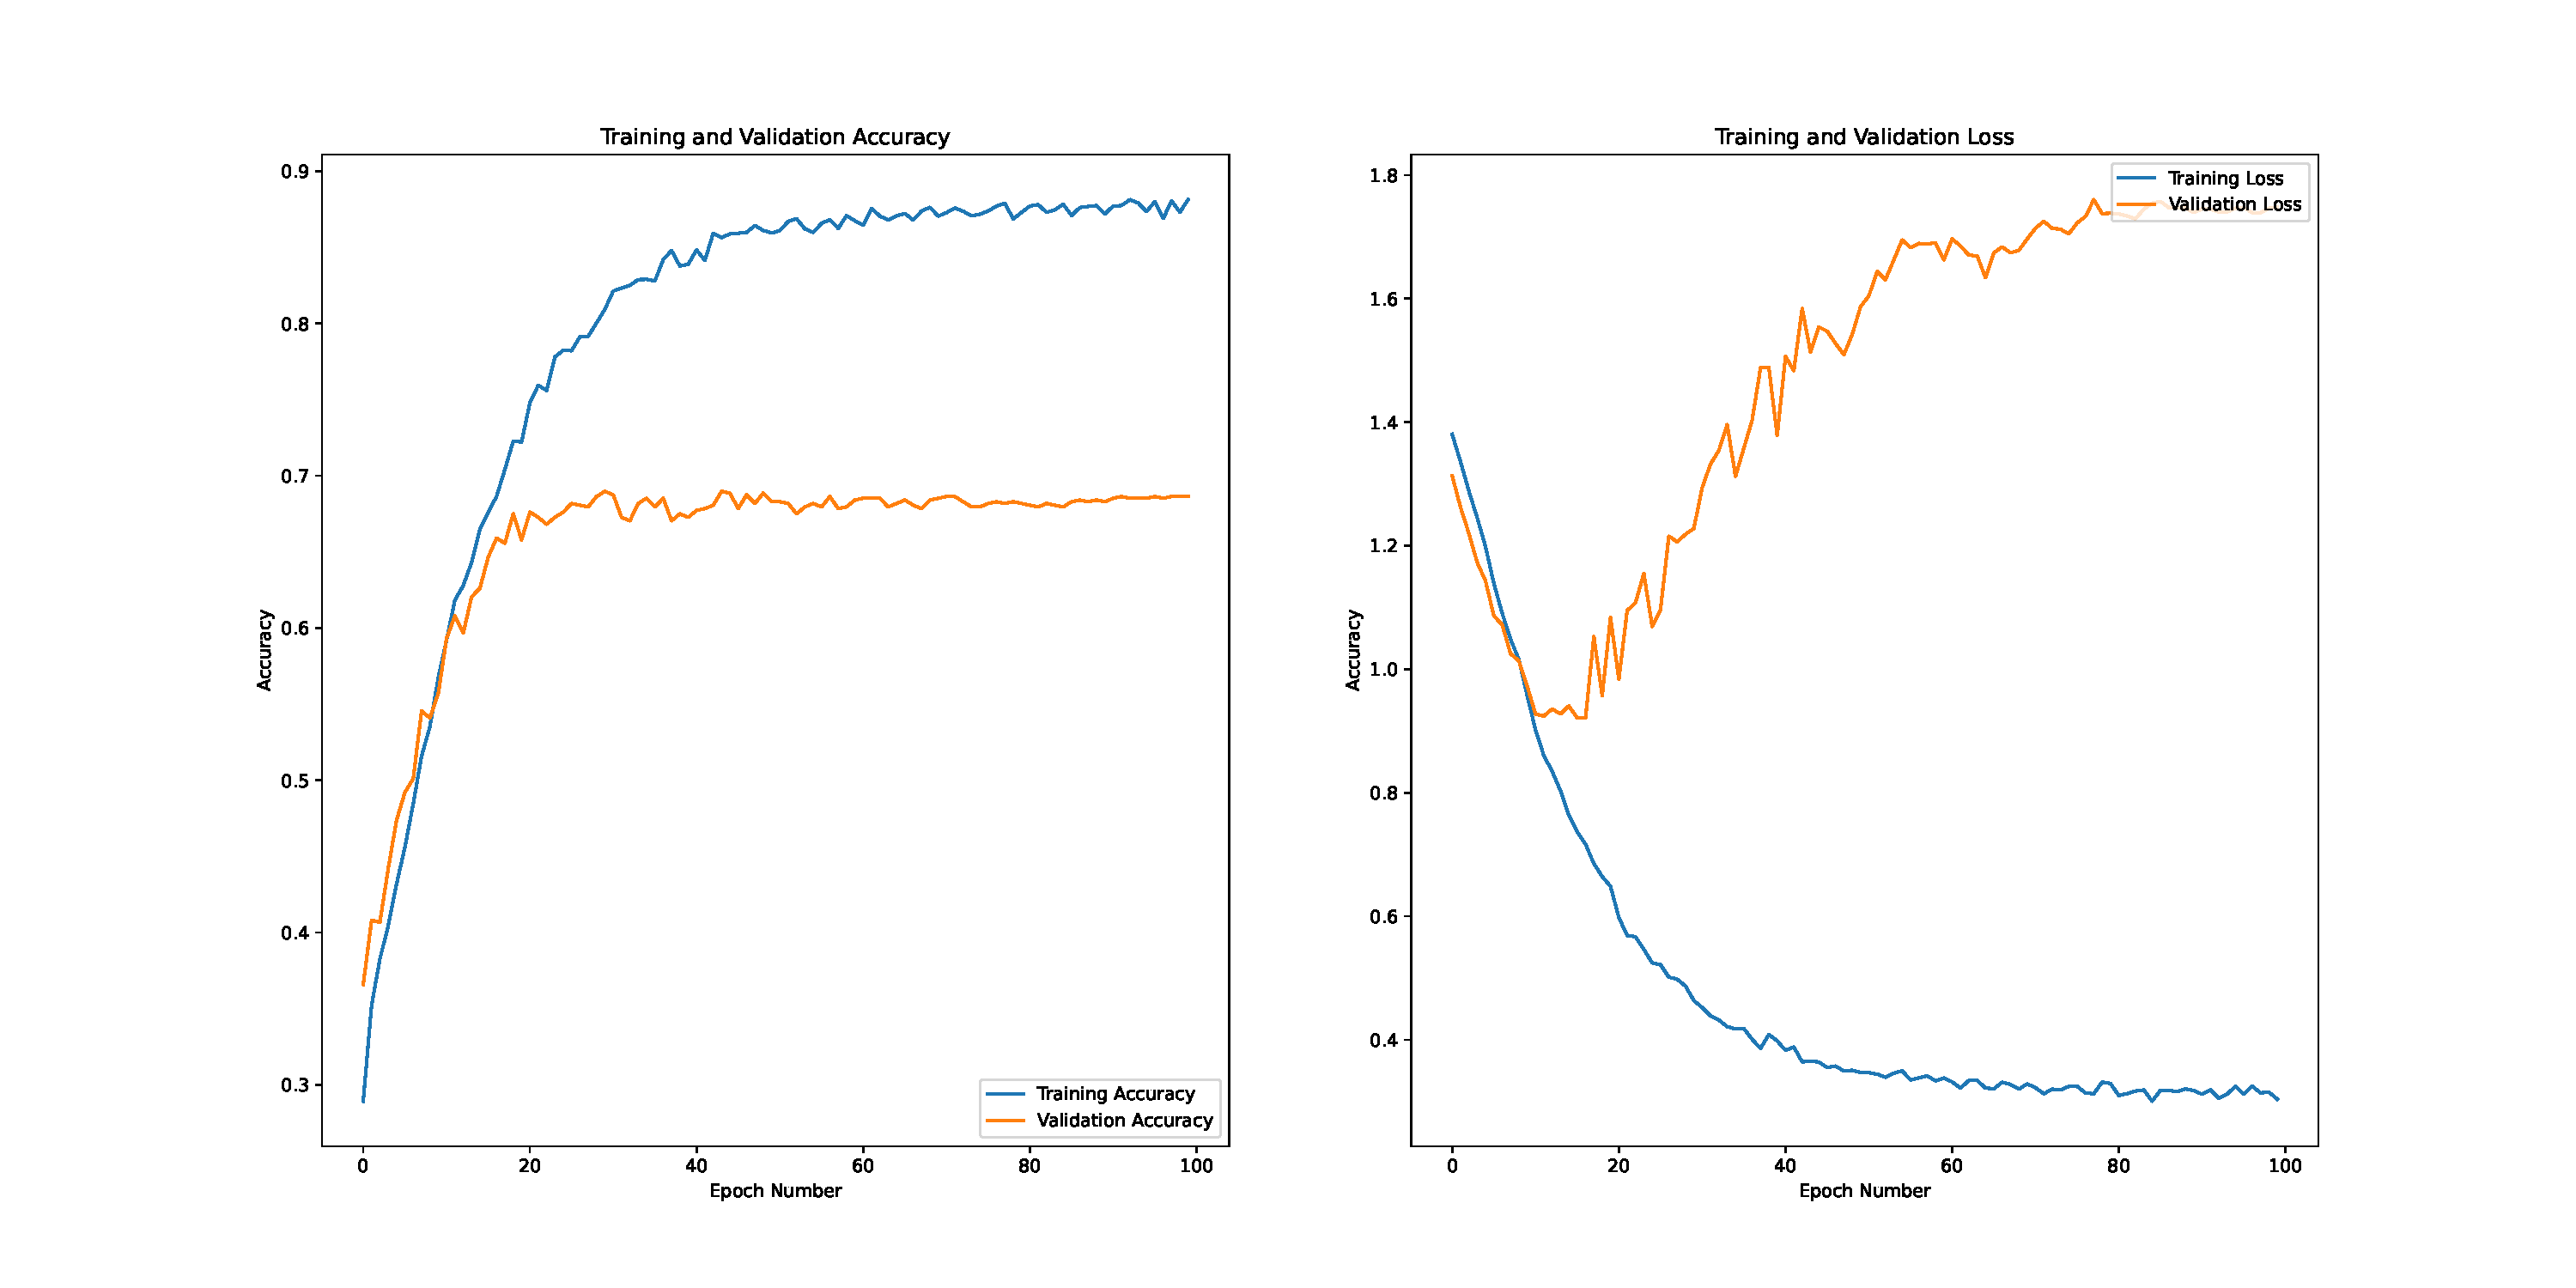
\includegraphics[width=0.5\textwidth]{metrics/4.2 metrics.pdf}}\\
    \subfloat[\centering Experiment 4.3. \acrshort{lr} multiplier equals 0.7.]{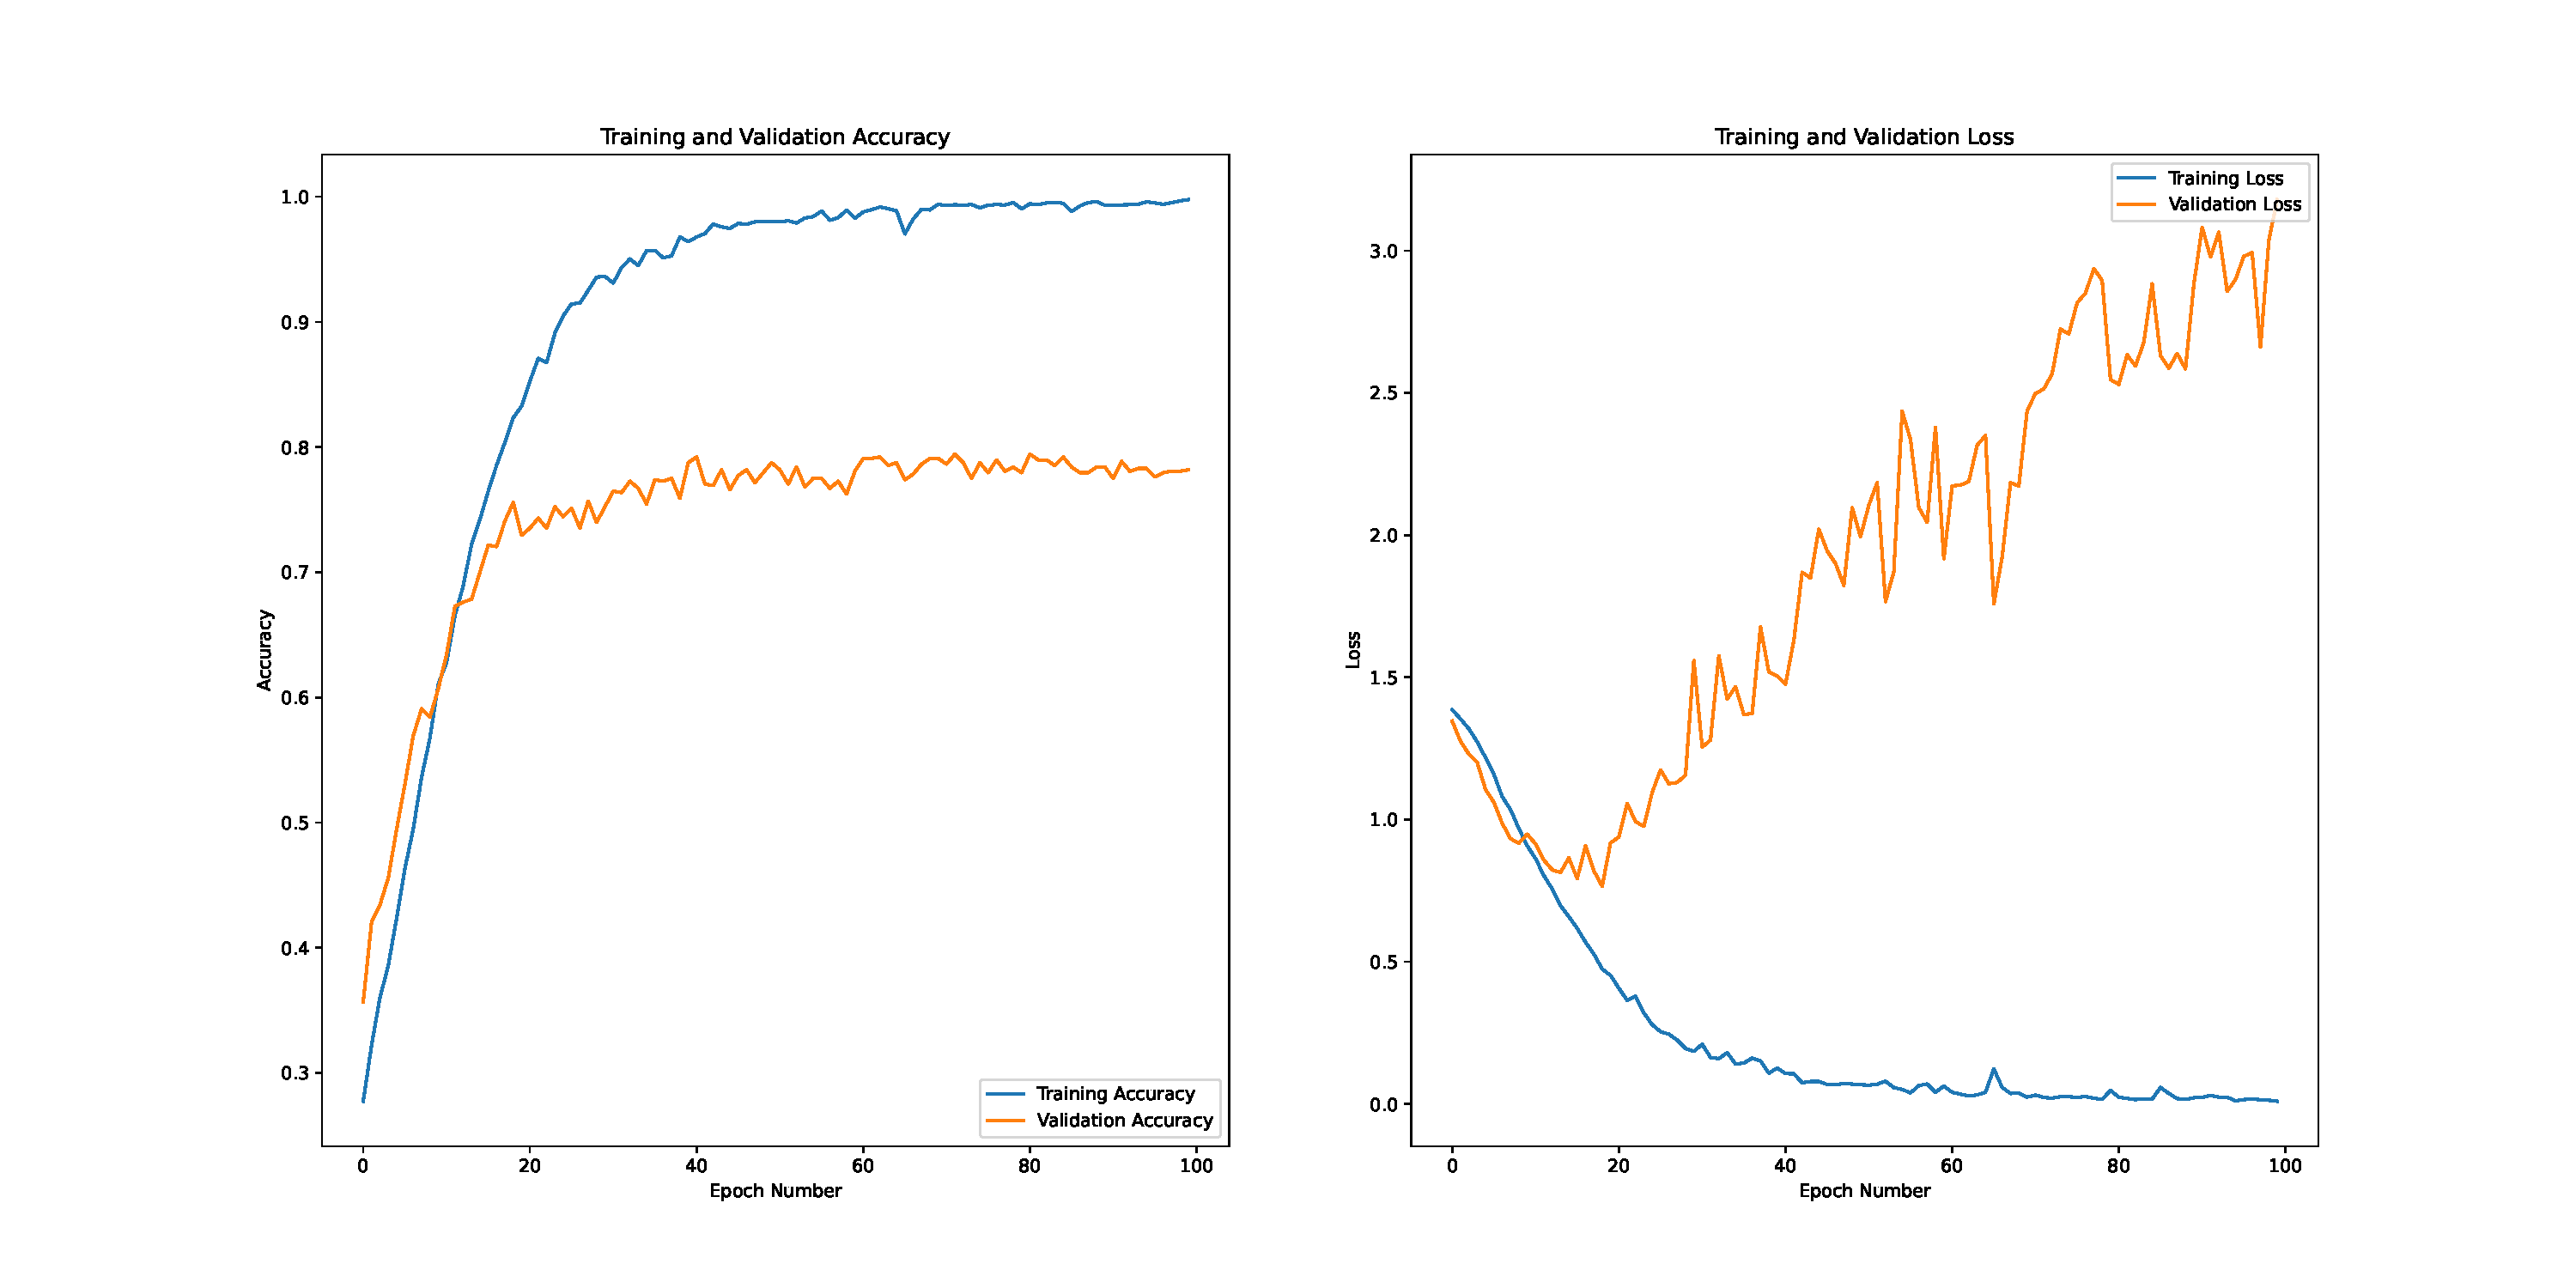
\includegraphics[width=0.5\textwidth]{metrics/4.3 metrics.pdf}}
\caption[Experiment 4 results]{Experiment 4 results. This depicts the three experiments with adaptive \acrshort{lr} via the Adam optimiser combined with a manual \acrshort{lr} change via a multiplier. All three experiments used an initial \acrshort{lr} of 0.0001 and multiplied the \acrshort{lr} every 20 epochs. Experiment 4.1 used a decay rate of 0.9, 4.2 used 0.5 and 4.3 used 0.7.}
\label{fig:4 results}
\end{figure}
\begin{table}
\centering
\begin{tabular}{|c|c|c|c|} 
 \hline
 Experiment &  Testing Accuracy & Testing Loss  & \acrshort{wer} \\ [0.2ex] 
 \hline
 4.1 & \accuracyfourone & \lossfourone & \werfourone \\
 4.2 & \accuracyfourtwo & \lossfourtwo & \werfourtwo \\
 4.3 & \accuracyfourthree & \lossfourthree & \werfourthree \\
 \hline
\end{tabular}
\caption{The testing accuracy, loss and \acrshort{wer} for experiment 4.}
\label{table: 4 results}
\end{table}
The results of the adaptive \acrshort{lr} experiment, represented in Figure~\ref{fig:4 results} and Table~\ref{table: 4 results}, show that altering the \acrshort{lr} significantly impacts the performance of models. The same model architecture but a different \acrshort{lr} scheduling method resulted in a much-improved model, as compared with Section~\ref{sec: Experiment 3} which just used the Adam optimiser.\\
The initial experiment, which employed 0.9 for the \acrshort{lr} multiplier, had an interesting performance. There is a large dip in performance where the model diverged and left the local minimum in the loss. The \acrshort{lr} was potentially changed too fast in this case.\\
A \acrshort{lr} multiplier of 0.5 reduced this effect, causing some \gls{overfitting} but not model divergence. Moreover, the accuracy and loss with this architecture spiked far less than with previous experiments and the testing metrics gave the best results seen yet.\\
A \acrshort{lr} multiplier of 0.7 strangely did not represent a middle-ground between the two experiments but instead a dip in performance. Because of this, the multiplier of 0.5 was applied to further experimentation.
\section{Experiment 5: Lip Landmarks}
\label{sec: Experiment 5}
% Experiment 8
% Only lip landmarks
\subsection{Model Architecture}
\begin{figure}
\centering
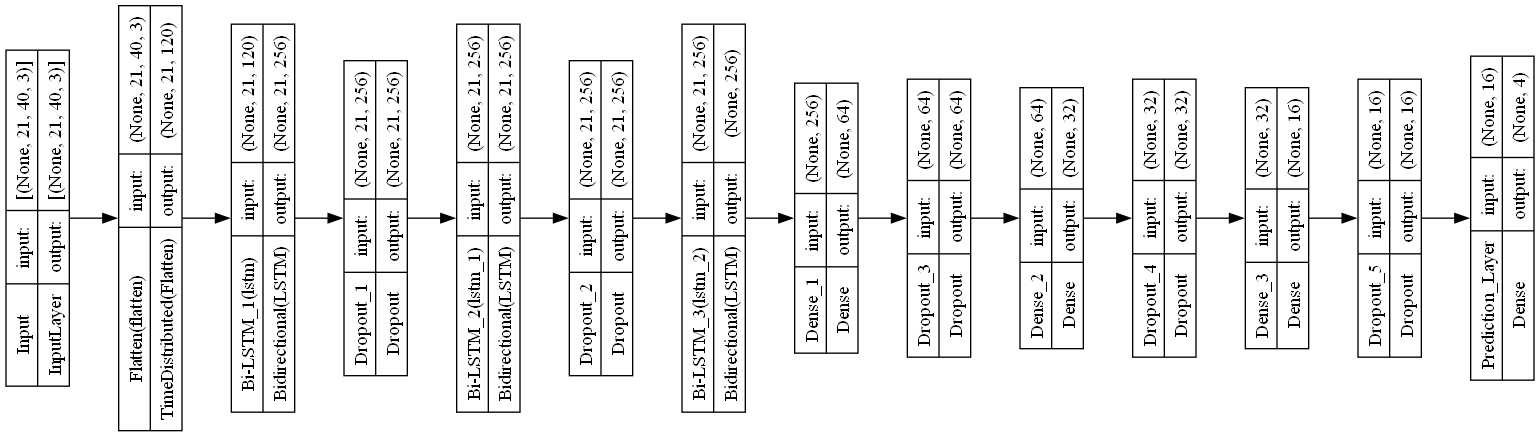
\includegraphics[width=0.9\textwidth]{model architectures/5 architecture.png}
\caption{Experiment 5 architecture.}
\label{fig:5 architecture}
\end{figure}
Previously, only visual features had been used for training. Alternatively, this experiment investigated the use of only landmark features as a model input.\\
As shown in Figure~\ref{fig:5 architecture}, the same model architecture was used as Section~\ref{sec: Experiment 4} except that the input size of the model was changed. Rather than accepting 2048 long feature vectors, the model had an input size of 120. This was formed of the 40 lip landmarks, represented with $(X, Y, Z)$ coordinates, as specified in Section~\ref{sec: Landmark Feature Extraction}.\\
Similarly to Section~\ref{sec: Experiment 4}, a set of sub-experiments were carried out to find the optimal performance of this architecture. The same model was used initially, to better compared with the previous experiment. The \acrshort{lr} was then altered to find optimal performance.\\
Various methods were utilised to schedule and vary the \acrshort{lr} throughout training. Whilst manual \acrshort{lr} scheduling had already been investigated, other settings were trialled. The Adam optimiser was employed for each experiment.\\
Experiment~5.1 used the same \acrshort{lr} scheduling as in experiment~4.2. Experiments~5.2 to 5.4 used different, manual \acrshort{lr} scheduling methods and 5.5 used exponential decay, as explained in Section~\ref{sec: Learning Rate}. Keras' exponential decay\footnote{\url{https://keras.io/api/optimizers/learning_rate_schedules/exponential_decay/}} was used to implement the decay method.
\subsection{Results and Evaluation}
\begin{figure}
\centering
    \subfloat[\centering Experiment 5.1.]{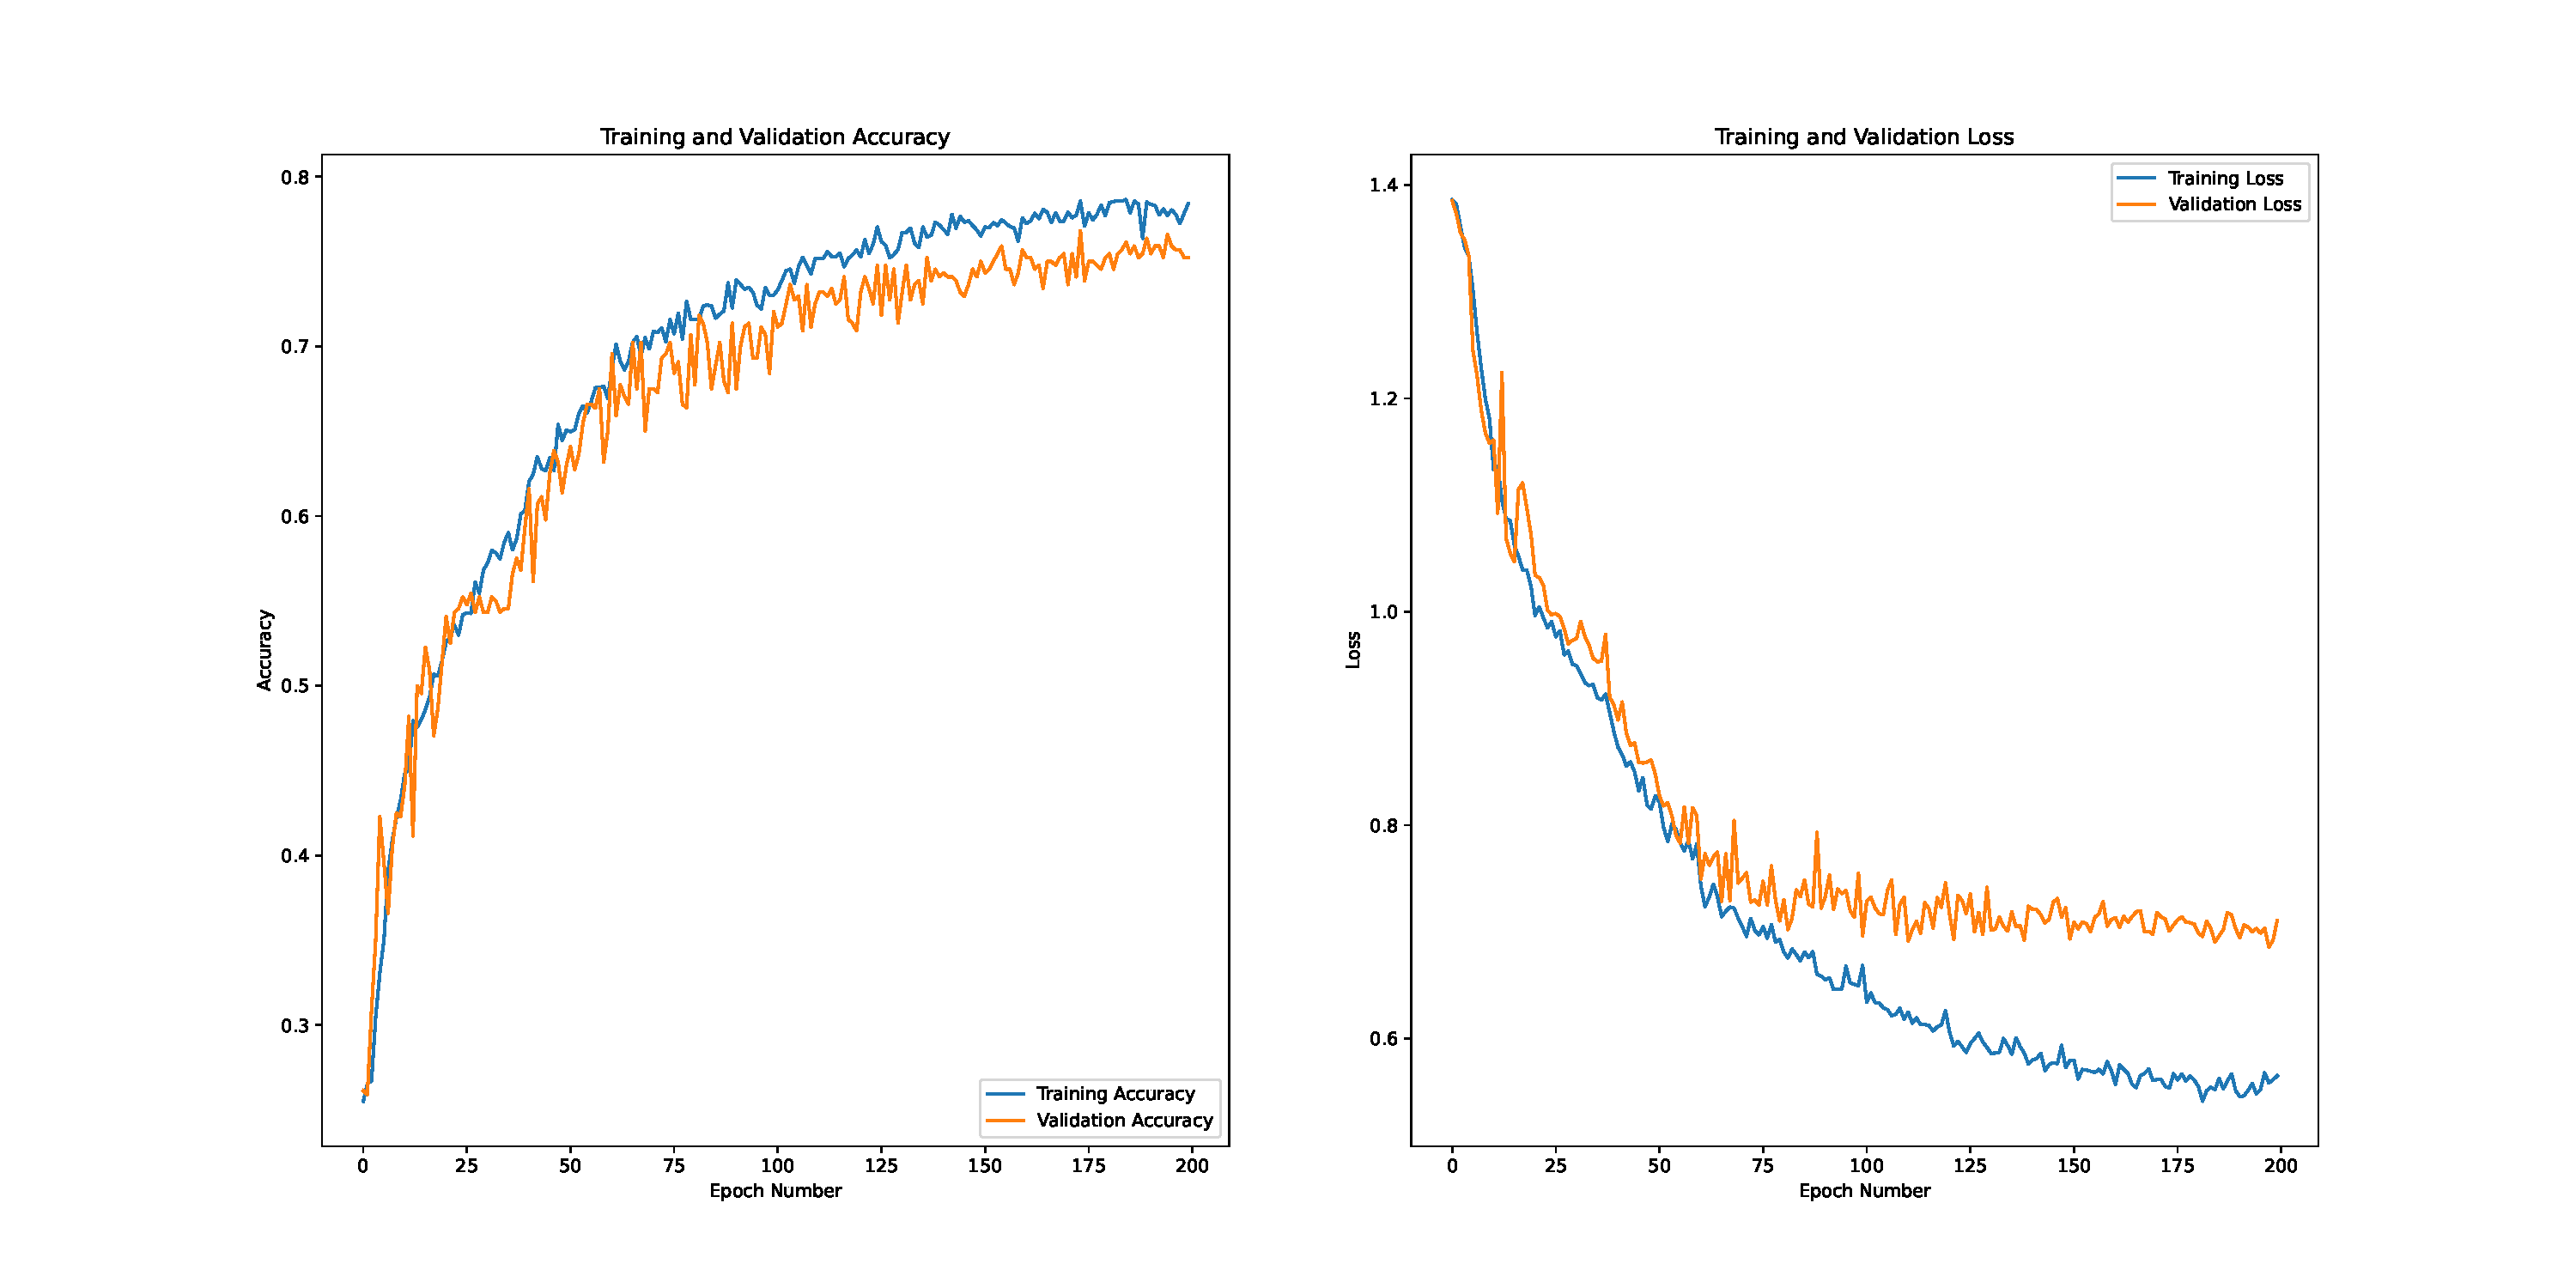
\includegraphics[width=0.5\textwidth]{metrics/5.1 metrics.pdf}}
    \subfloat[\centering Experiment 5.2.]{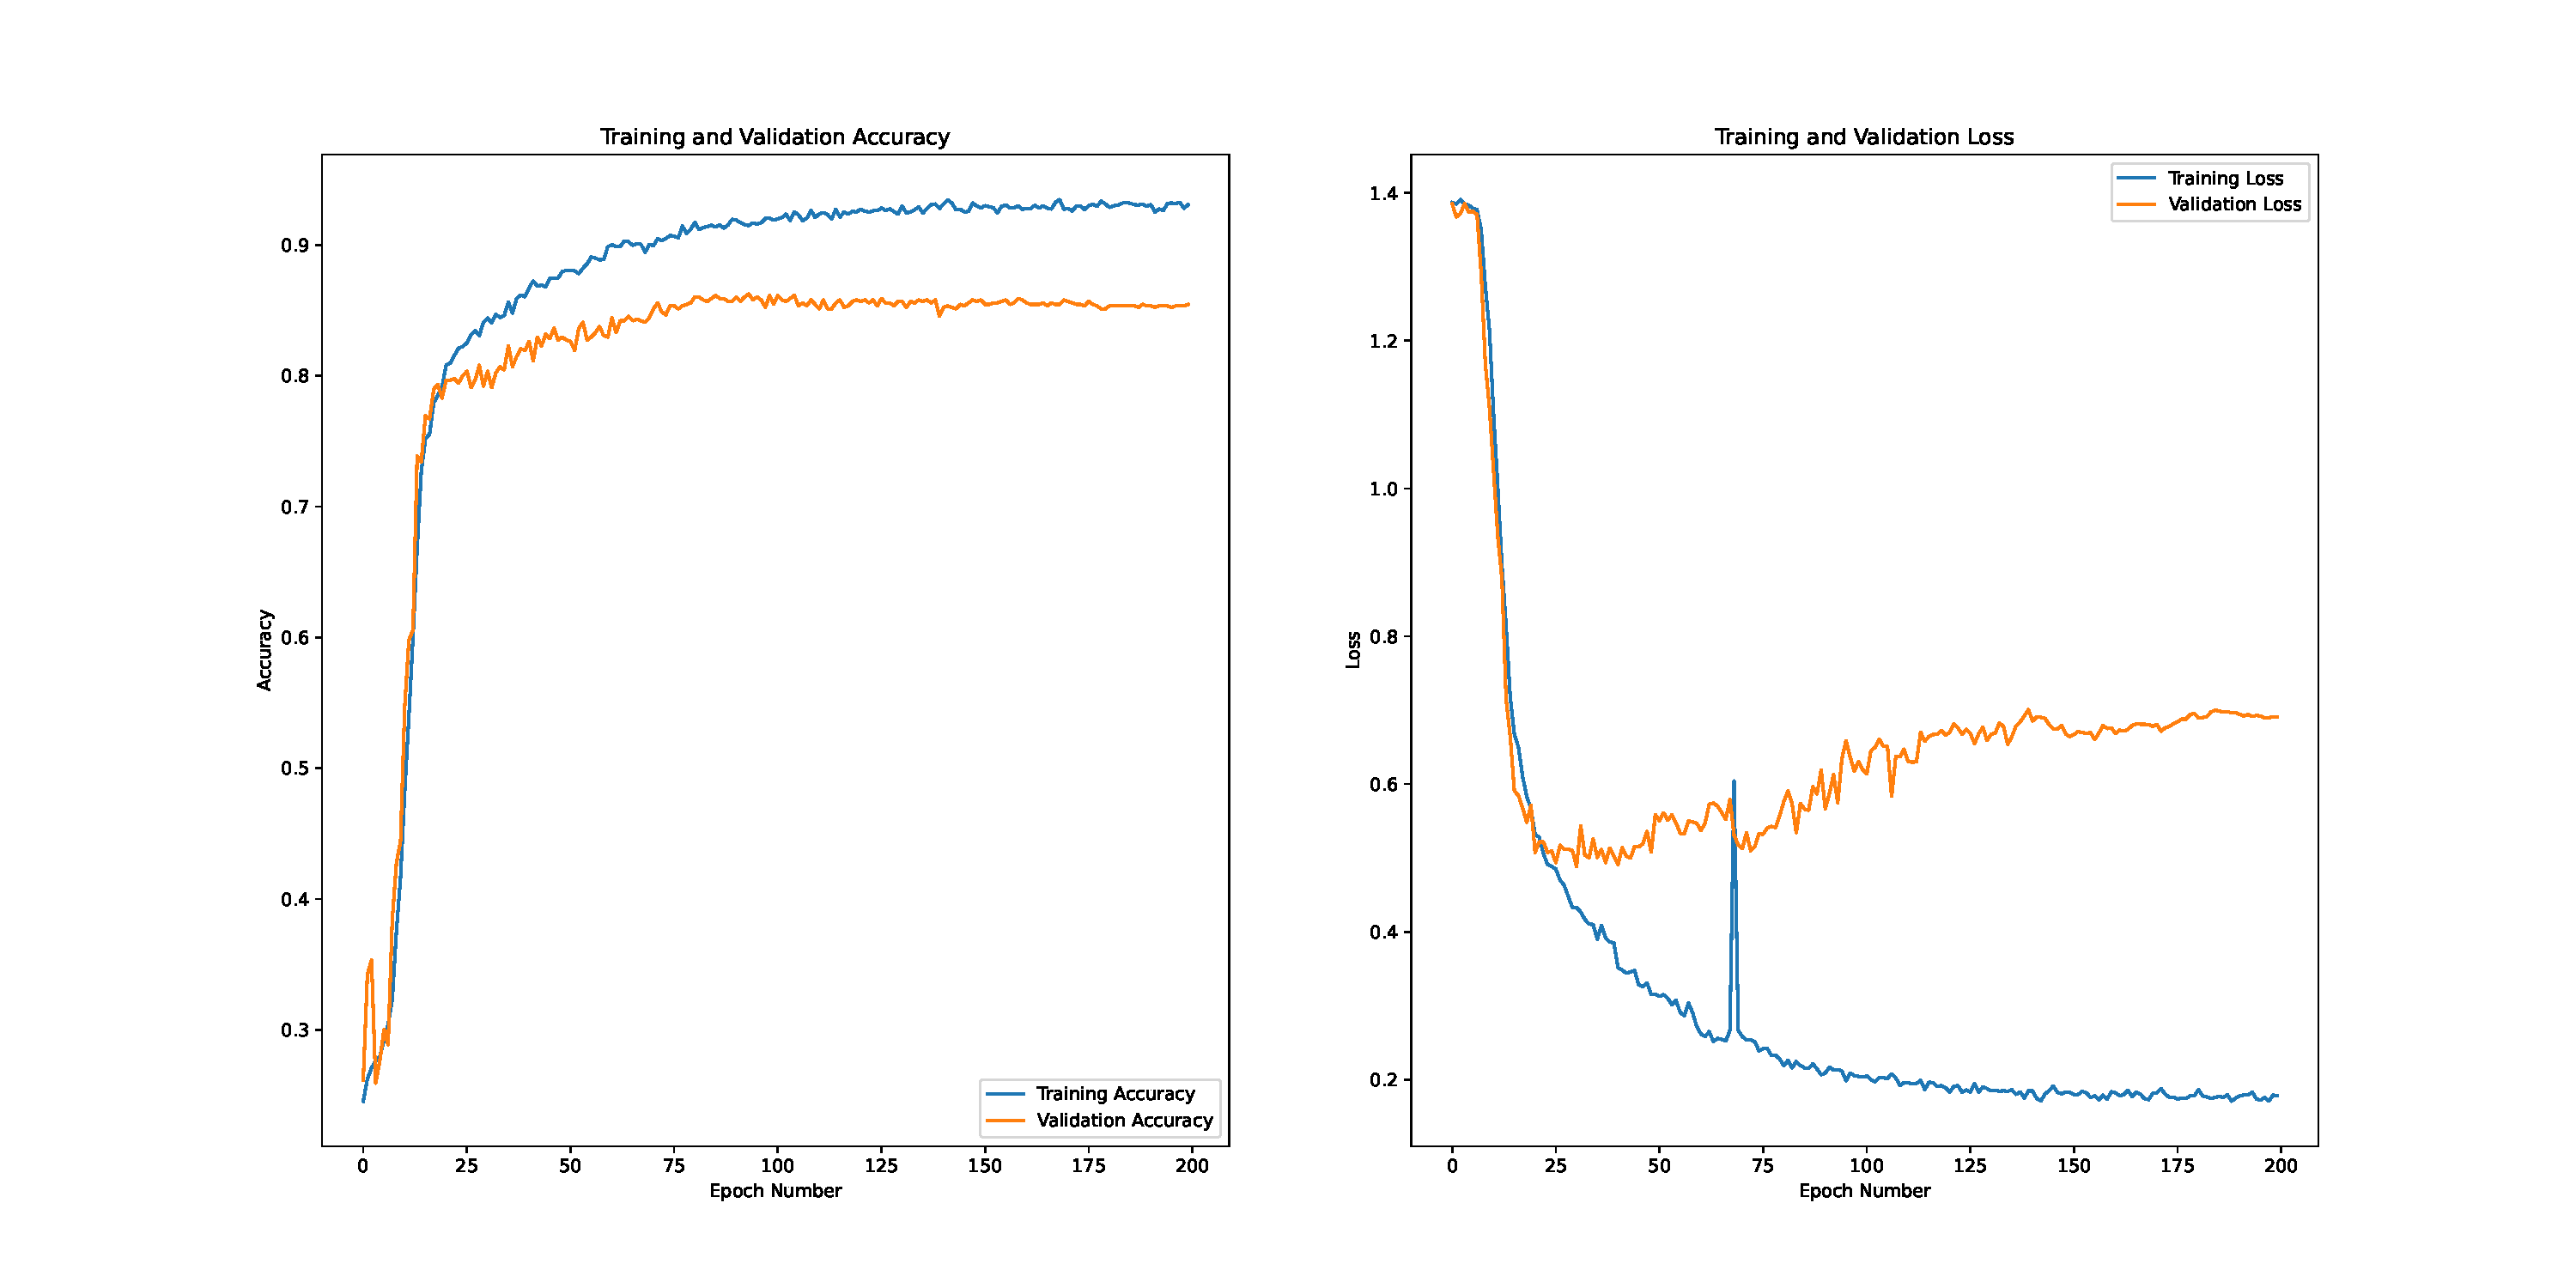
\includegraphics[width=0.5\textwidth]{metrics/5.2 metrics.pdf}}\\
    \subfloat[\centering Experiment 5.3.]{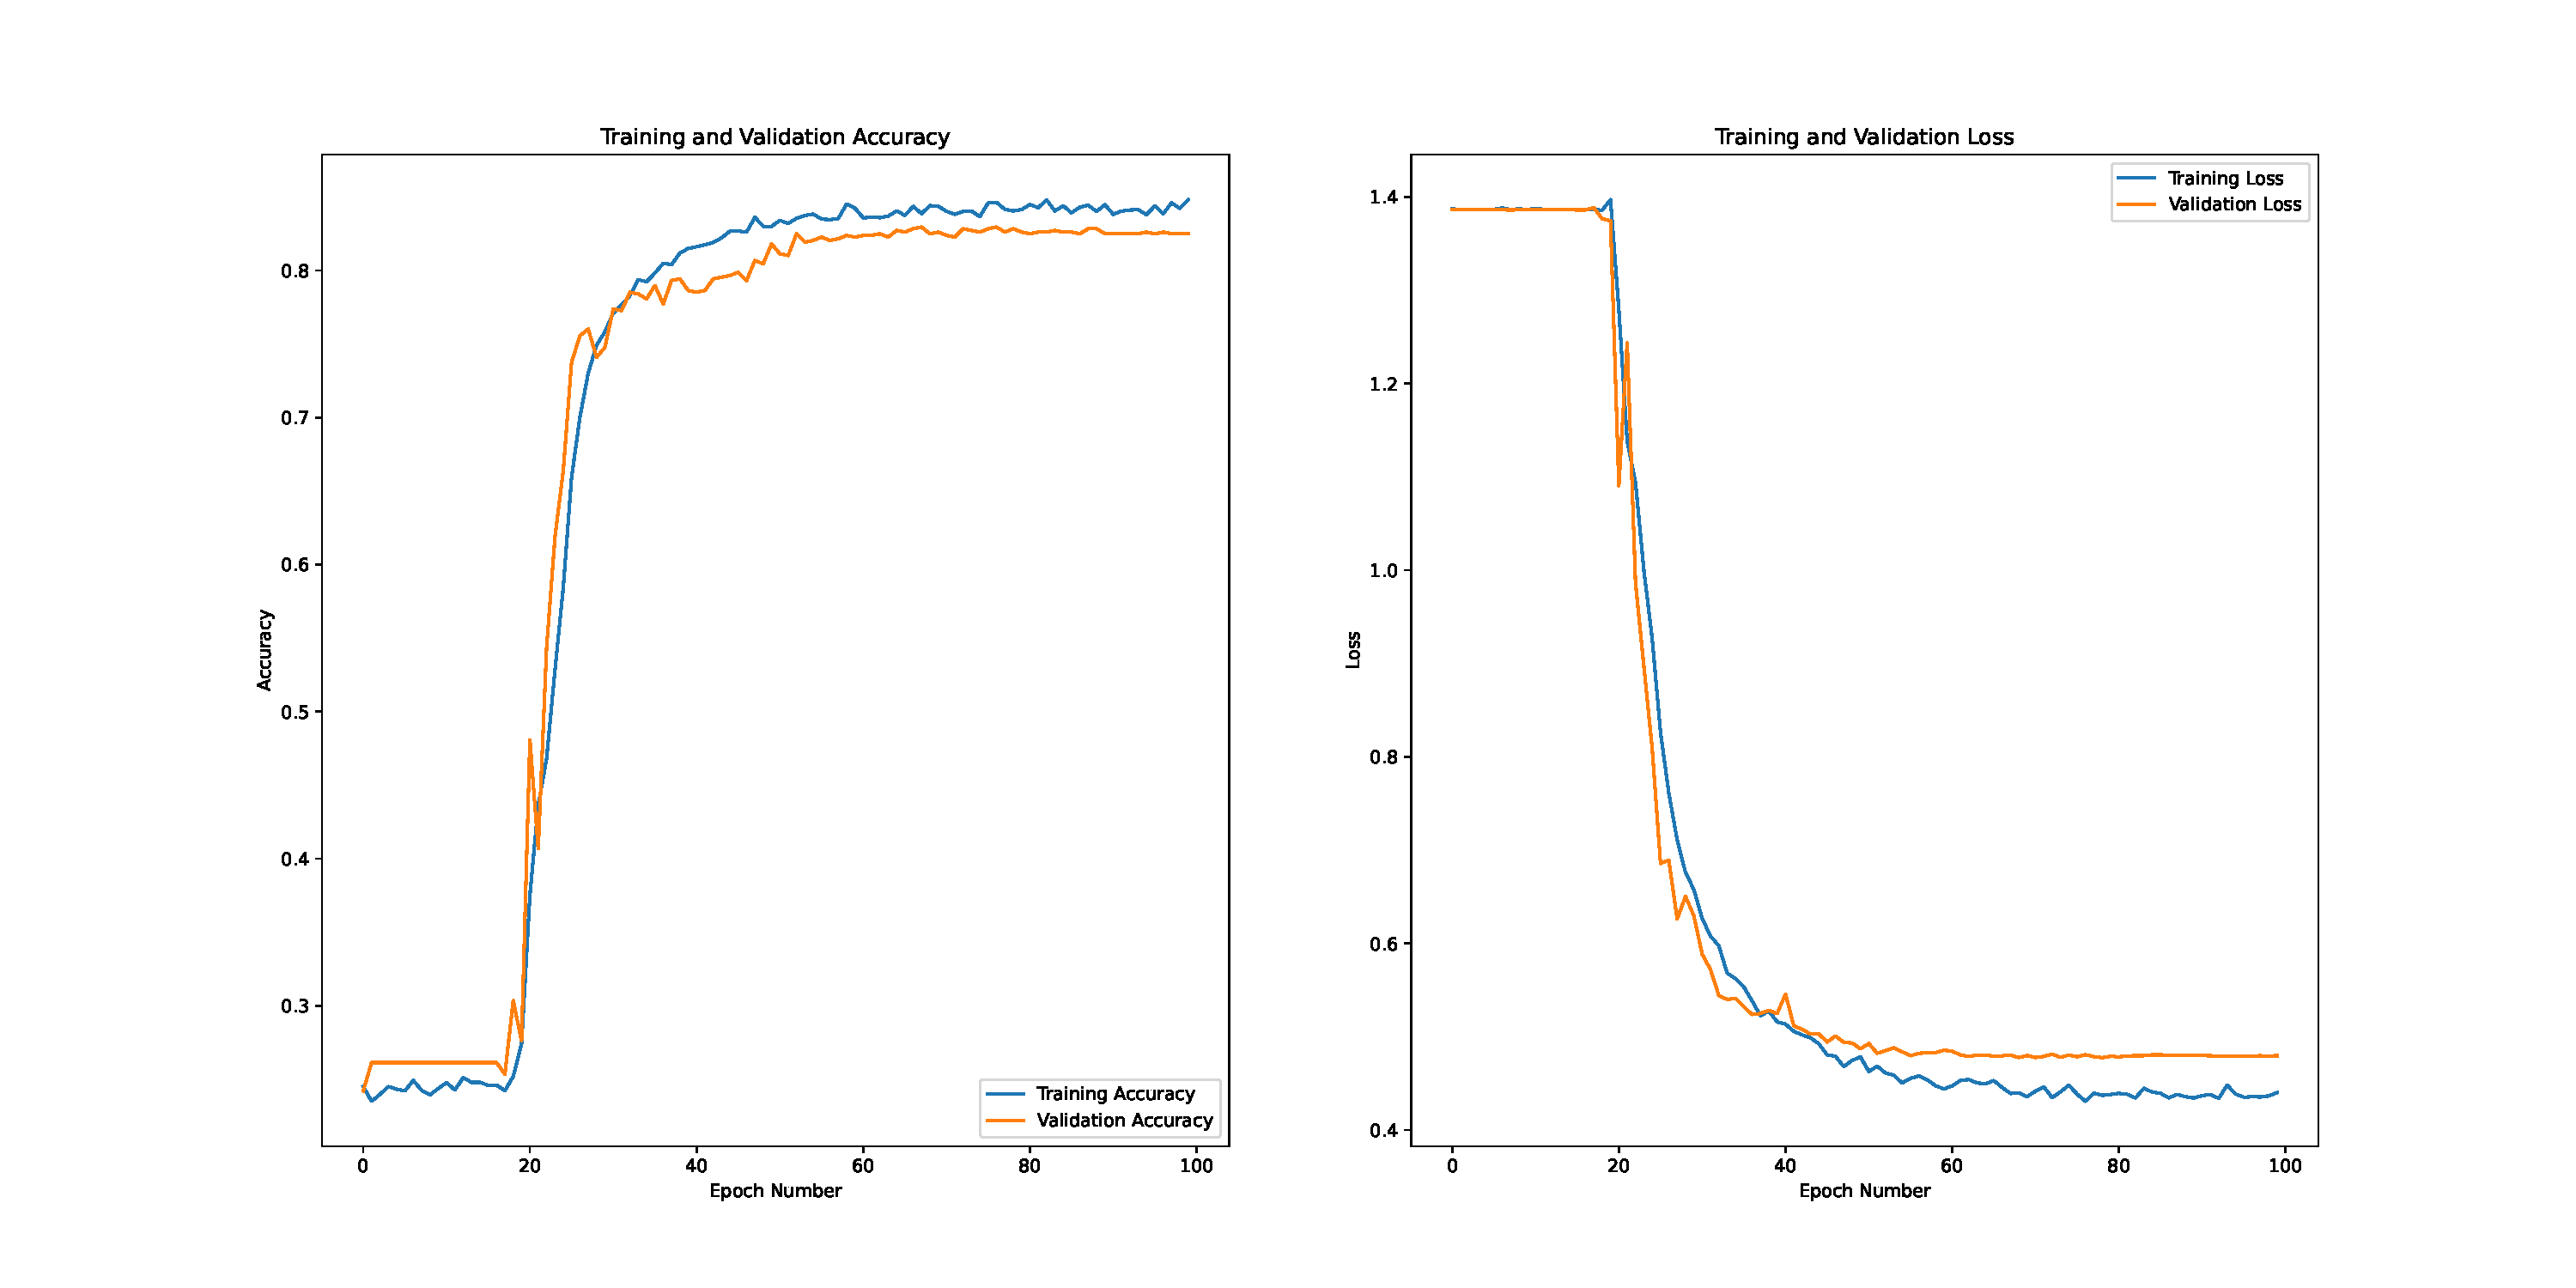
\includegraphics[width=0.5\textwidth]{metrics/5.3 metrics.pdf}}
    \subfloat[\centering Experiment 5.4.]{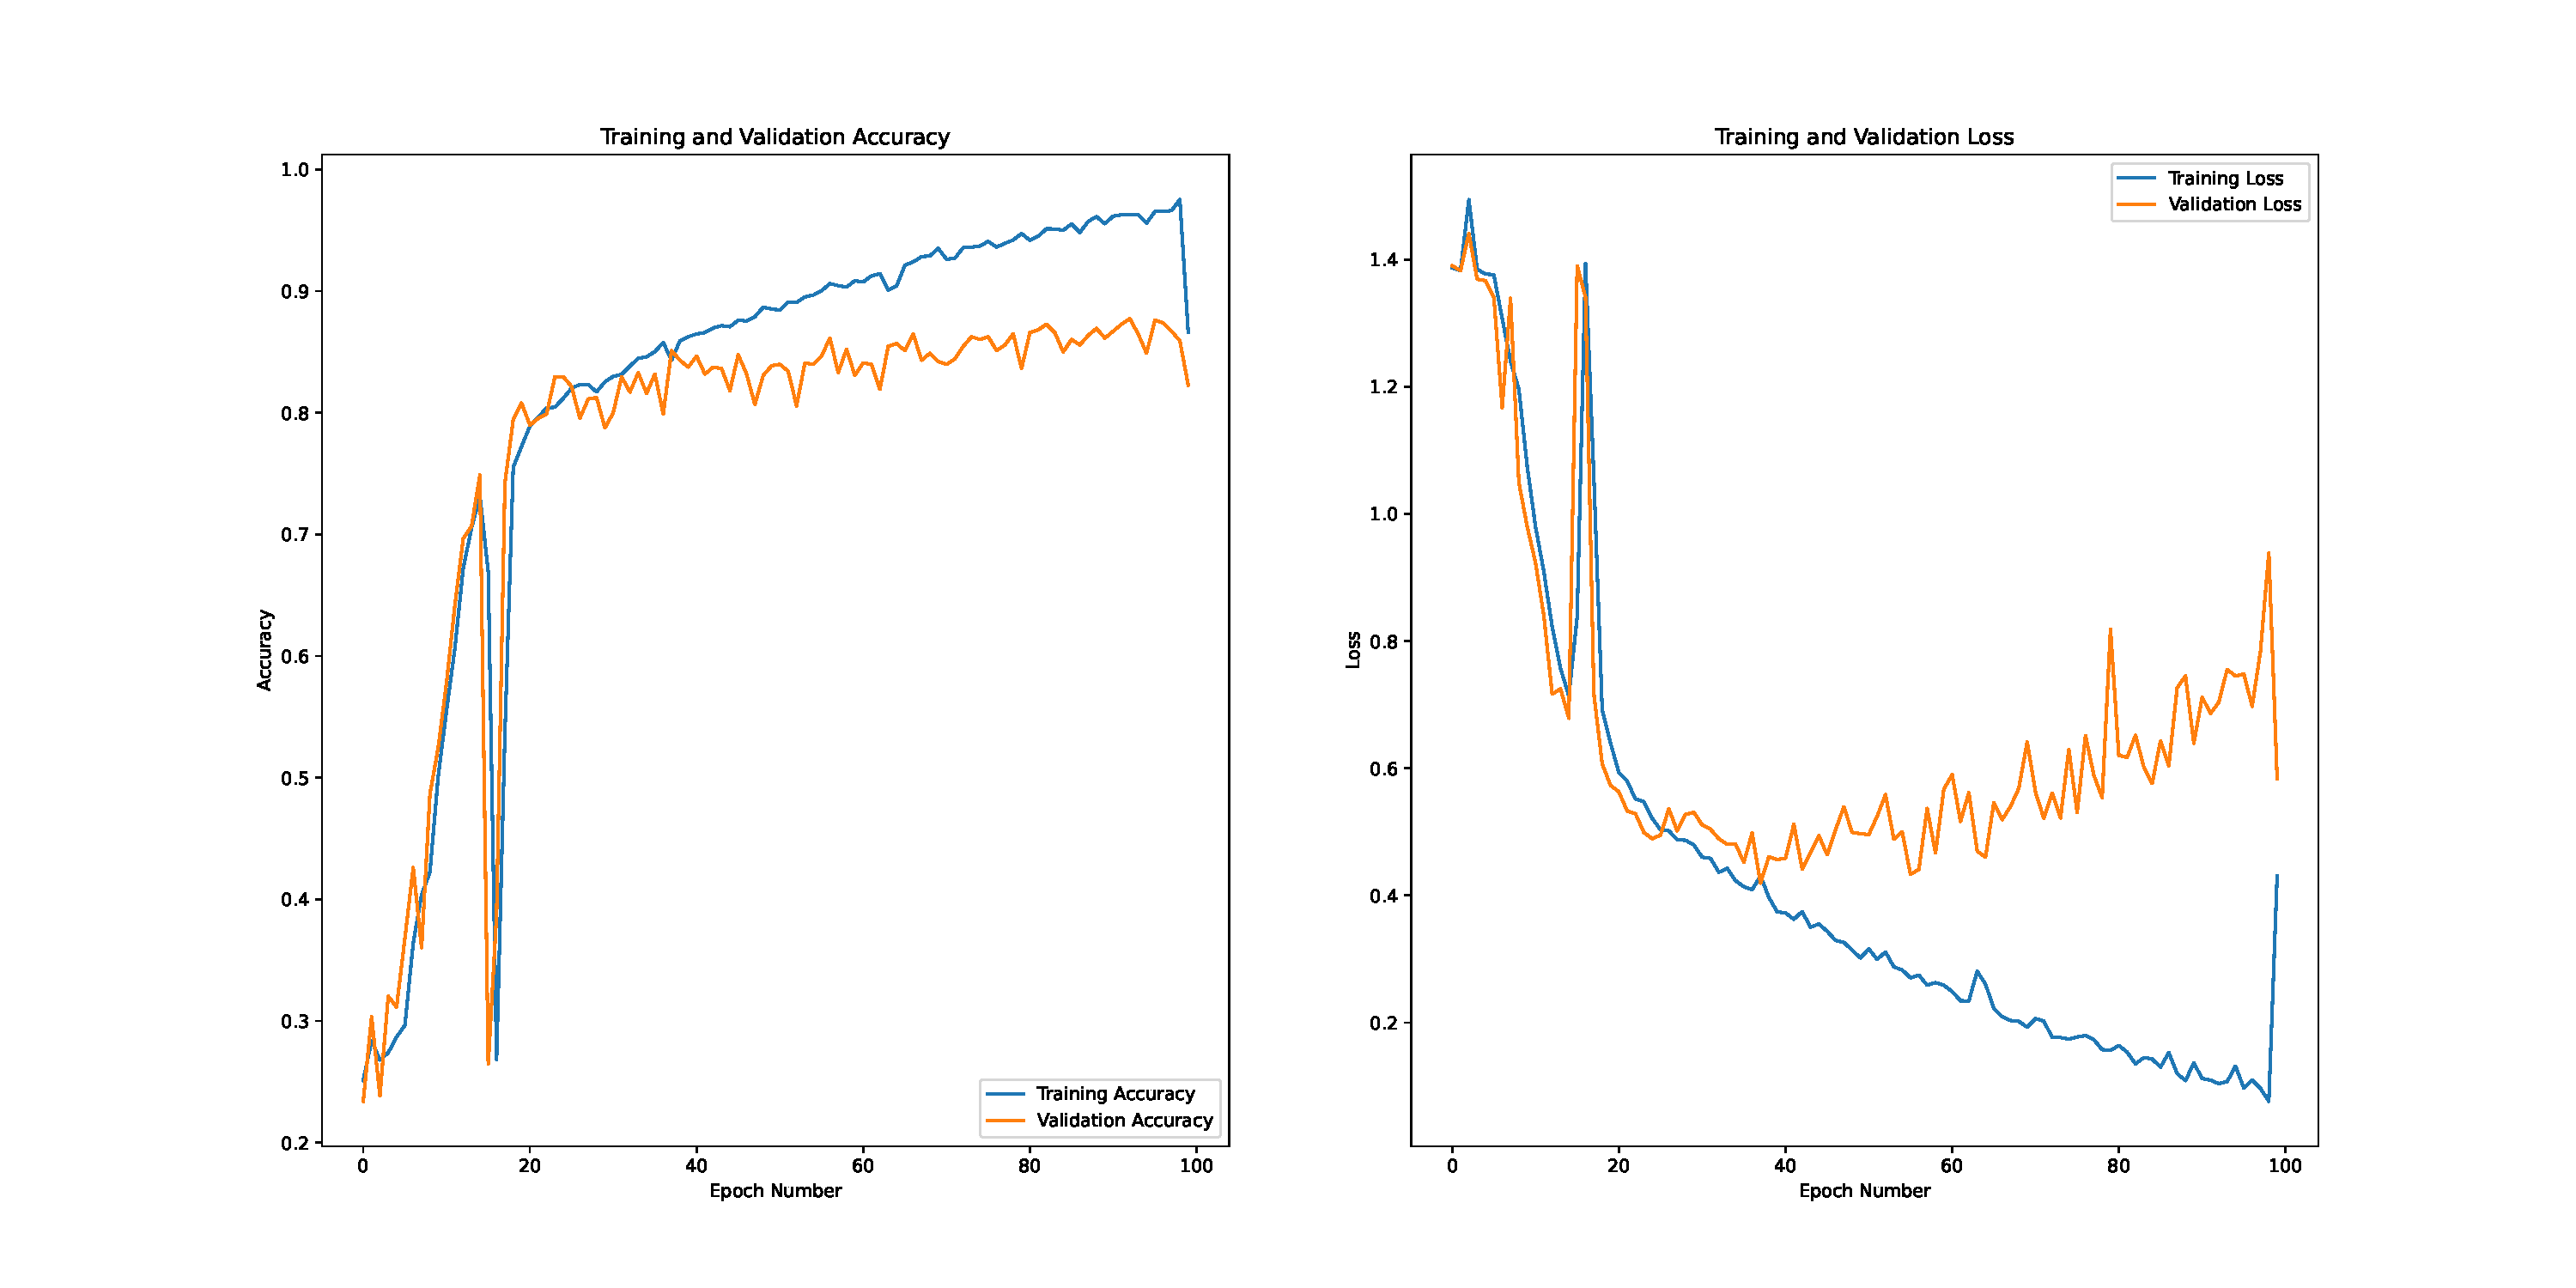
\includegraphics[width=0.5\textwidth]{metrics/5.4 metrics.pdf}}\\
    \subfloat[\centering Experiment 5.5.]{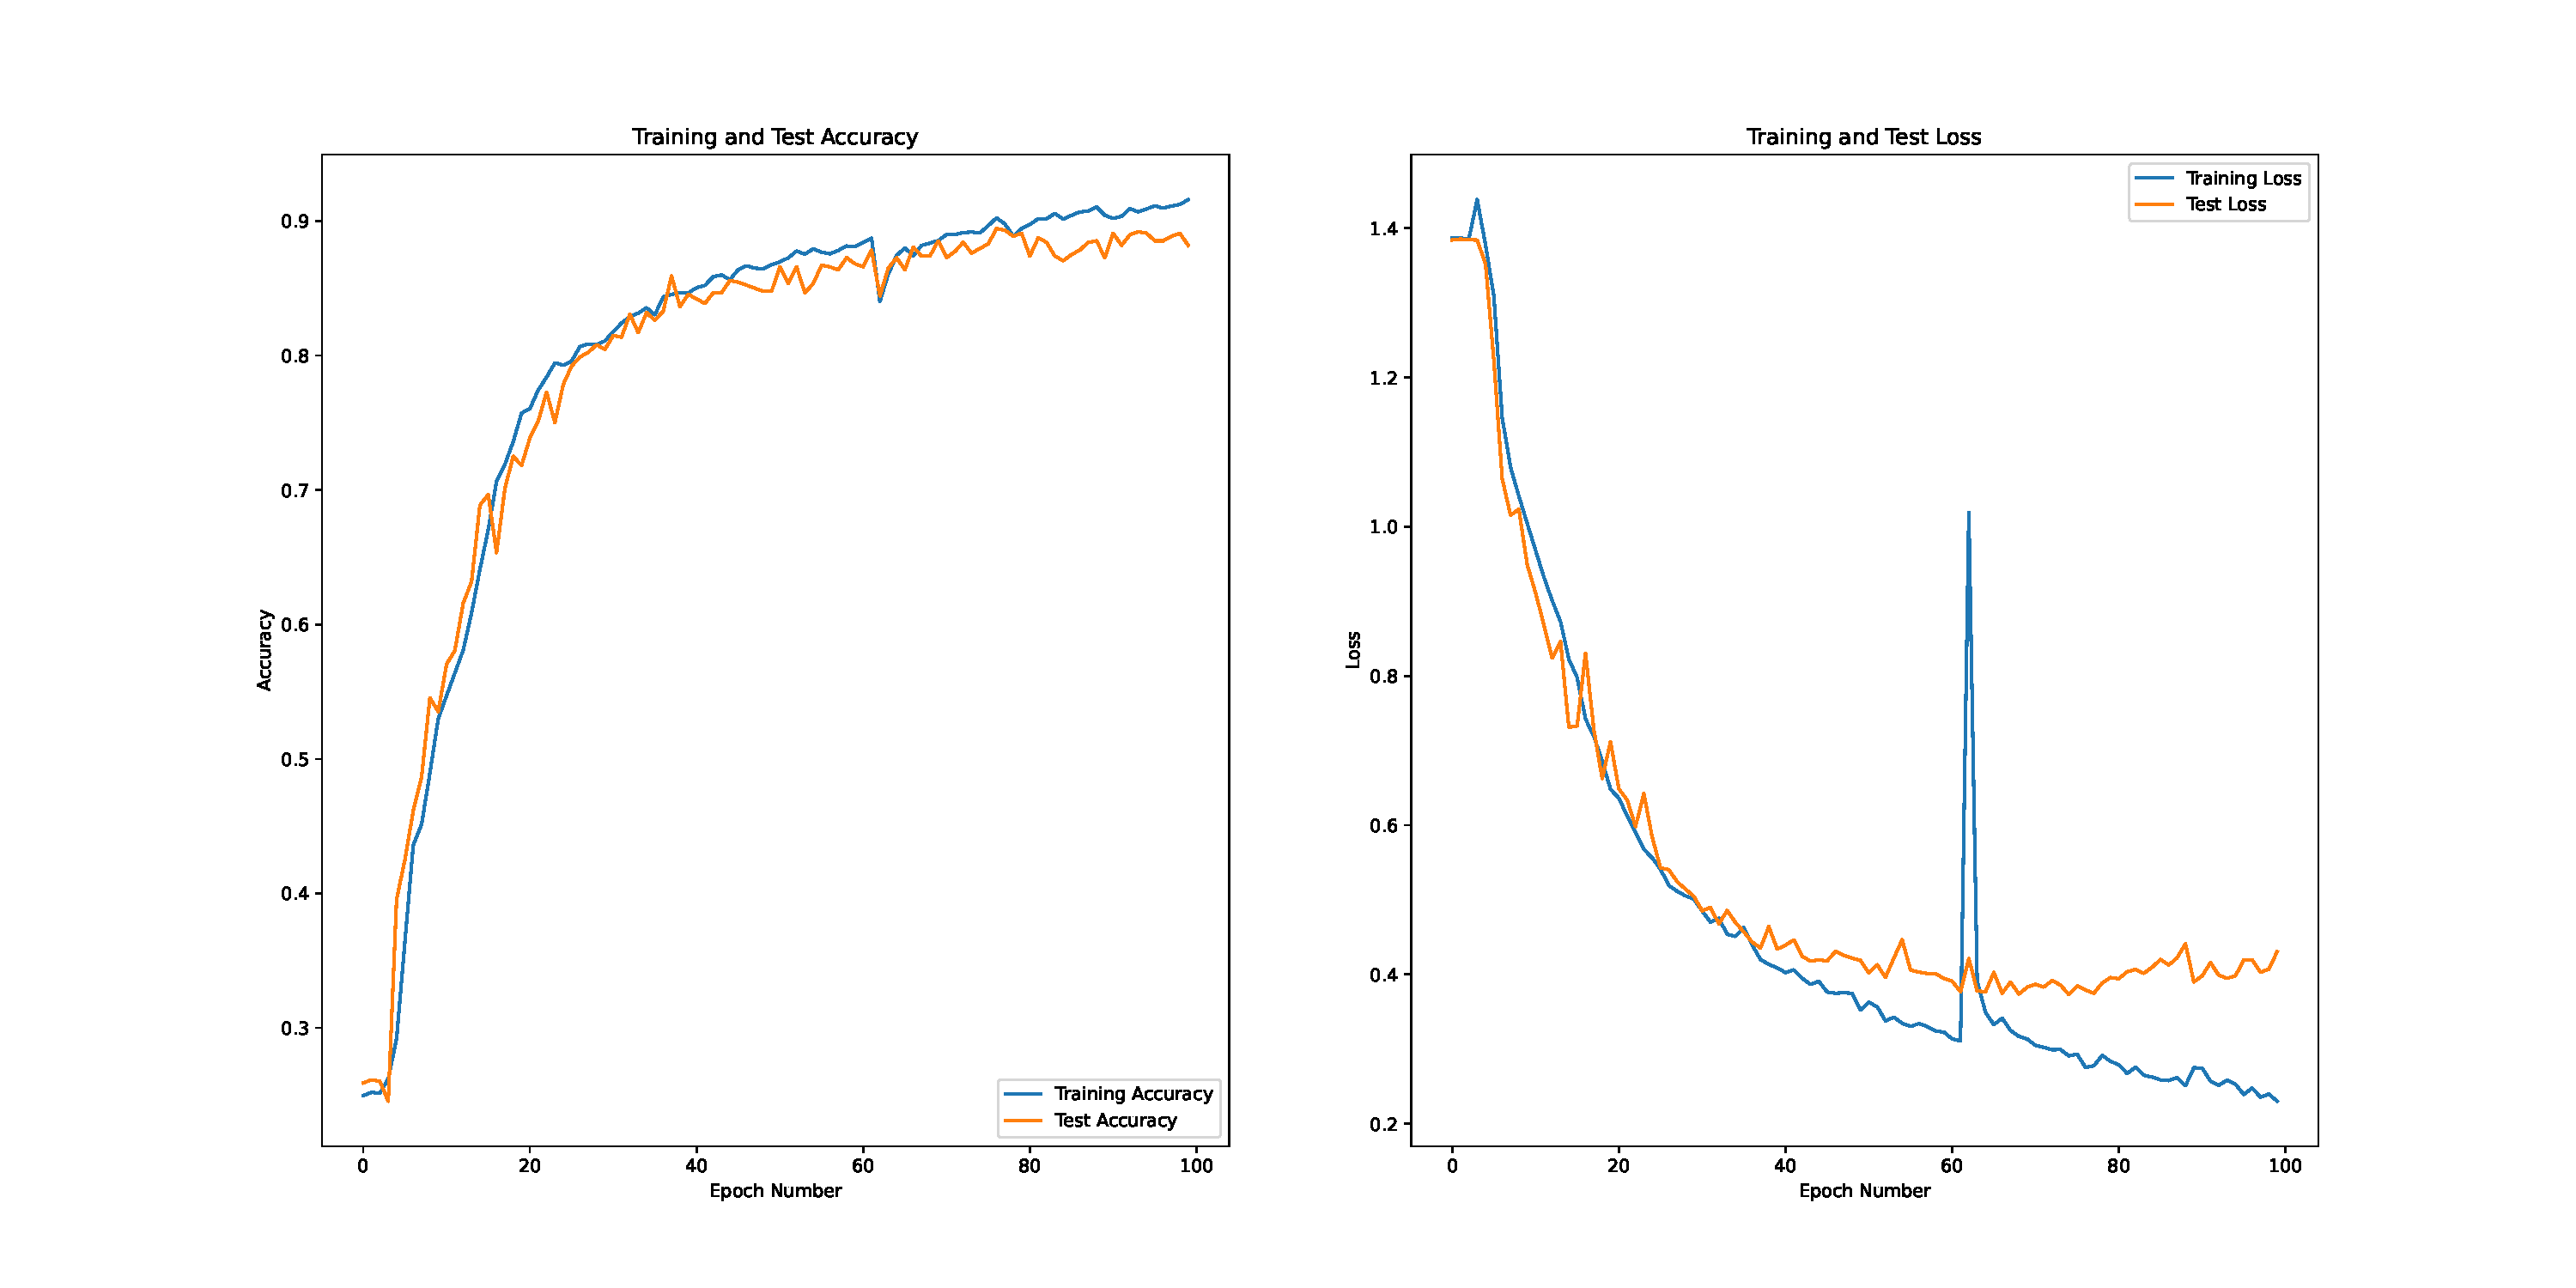
\includegraphics[width=0.5\textwidth]{metrics/5.5 metrics.pdf}}
\caption[Experiment 5 results]{Experiment 5 results. This depicts experiments~5.1, 5.2, 5.3, 5.4 and 5.5. Each of these experiments utilised the same model architecture but varying \acrshort{lr} scheduling methods. 5.1--5.4 utilised manual methods of changing the \acrshort{lr} whilst 5.5 showcased exponential decay.}
\label{fig:5 results}
\end{figure}
\begin{table}
\centering
\begin{tabular}{|c|p{35mm}|c|c|c|} 
 \hline
 Experiment & \acrshort{lr} Configuration & Testing Accuracy & Testing Loss & \acrshort{wer} \\ [0.2ex] 
 \hline
 5.1 & \textbf{Scheduler}: Manual\newline \textbf{Initial \acrshort{lr}}: 0.0001\newline \textbf{Change steps}: 20\newline \textbf{\acrshort{lr} change}: 0.5& \accuracyfiveone & \lossfiveone & \werfiveone \\ 
 \hline
 5.2 & \textbf{Scheduler}: Manual\newline \textbf{Initial \acrshort{lr}}: 0.001\newline \textbf{Change steps}: 20\newline \textbf{\acrshort{lr} change}: 0.5& \accuracyfivetwo & \lossfivetwo & \werfivetwo \\ 
 \hline
 5.3 & \textbf{Scheduler}: Manual\newline \textbf{Initial \acrshort{lr}}: 0.001\newline \textbf{Change steps}: 30\newline \textbf{\acrshort{lr} change}: $e^{-0.1}$& \accuracyfivethree & \lossfivethree & \werfivethree \\ 
 \hline
 5.4 & \textbf{Scheduler}: Manual\newline \textbf{Initial \acrshort{lr}}: 0.001\newline \textbf{Change steps}: 30\newline \textbf{\acrshort{lr} change}: $e^{-0.01}$ & \accuracyfivefour & \lossfivefour & \werfivefour \\ \hline
 5.5 & \textbf{Scheduler}: Exponential decay\newline \textbf{Initial \acrshort{lr}}: 0.001\newline \textbf{Decay steps}: 275\newline \textbf{Decay rate}: 0.9 & \accuracyfivefive & \lossfivefive & \werfivefive \\ 
 \hline
\end{tabular}
\caption[The testing accuracy, loss and \acrshort{wer} for experiment 5]{The testing accuracy, loss and \acrshort{wer} for experiment 5. This shows the settings for each of the different sub-experiments and the resulting testing accuracy and loss.}
\label{table: 5 results}
\end{table}
Although experiment~5.1 did not have improved performance compared with experiment~4.2, the findings from this experiment showed that landmark features are a suitable input for training lip reading models.\\
The reduced performance could be related to the reduced size of the input feature vectors or due to MediaPipe's accuracy. A low probability threshold was utilised during data generation and therefore it could be that the lip landmarks were less accurate than desired. This problem is not present when using visual features, which are just crops of the mouth region.\\
After this finding, different values for the \acrshort{lr} scheduling were assessed to optimise this model further, the results for which are represented within Figure~\ref{fig:5 results} and Table~\ref{table: 5 results}.\\
The next four experiments showed the impact of tuning the scheduler's parameters, significantly altering the performance of the model. When manually altering the \acrshort{lr}, starting with a higher initial \acrshort{lr} and a larger decay rate (leading to smaller changes in the \acrshort{lr}) performed better. Furthermore, Exponential decay performed very well, producing one of the best models in this research yet.\\
The \acrshort{lr} setting presented in experiment~5.4 performed the best. However, the \acrshort{lr} scheduler from experiment~5.5 was taken forwards. Although this model had worse testing metrics, the spiking within the accuracy and loss was far decreased compared with the other methods. Additionally, \gls{overfitting} appeared to have been diminished. This reliability is more useful than hyperparameters configured for a specific experiment. Experiment~5.5's \acrshort{lr} scheduling is more general and thus will be carried forward, rather than the settings for experiment~5.5.
\section{Experiment 6: Data Augmentation}
\label{sec: Experiment 6}
% Experiment 11
% More \gls{data_augmentation} 
\subsection{Model Architecture}
In Section~\ref{sec: Experiment 5}, although \gls{overfitting} was reduced, there was still divergence among the loss and accuracy in the later epochs. Thus, further methods of \gls{data_augmentation} were assessed to reduce this effect.\\
The method of \gls{data_augmentation} that was employed was a set of random rotations. Each of the data samples were randomly rotated and the new samples were added again to the dataset, to bolster the amount of training data. The same rotation was applied to each lip landmark within a frame, and each frame of a given video. The rotations were in the range $[-\frac{\pi}{8}, -0.1]$ and $[0.1, \frac{\pi}{8}]$. This was to ensure that the generated samples were not too similar to the originals. Normally, viewers will be upright and not rotated, so rotations were kept minimal.\\
Otherwise, the architecture for this experiment was identical to experiment~5.5.
\subsection{Results and Evaluation}
\begin{figure}
\centering
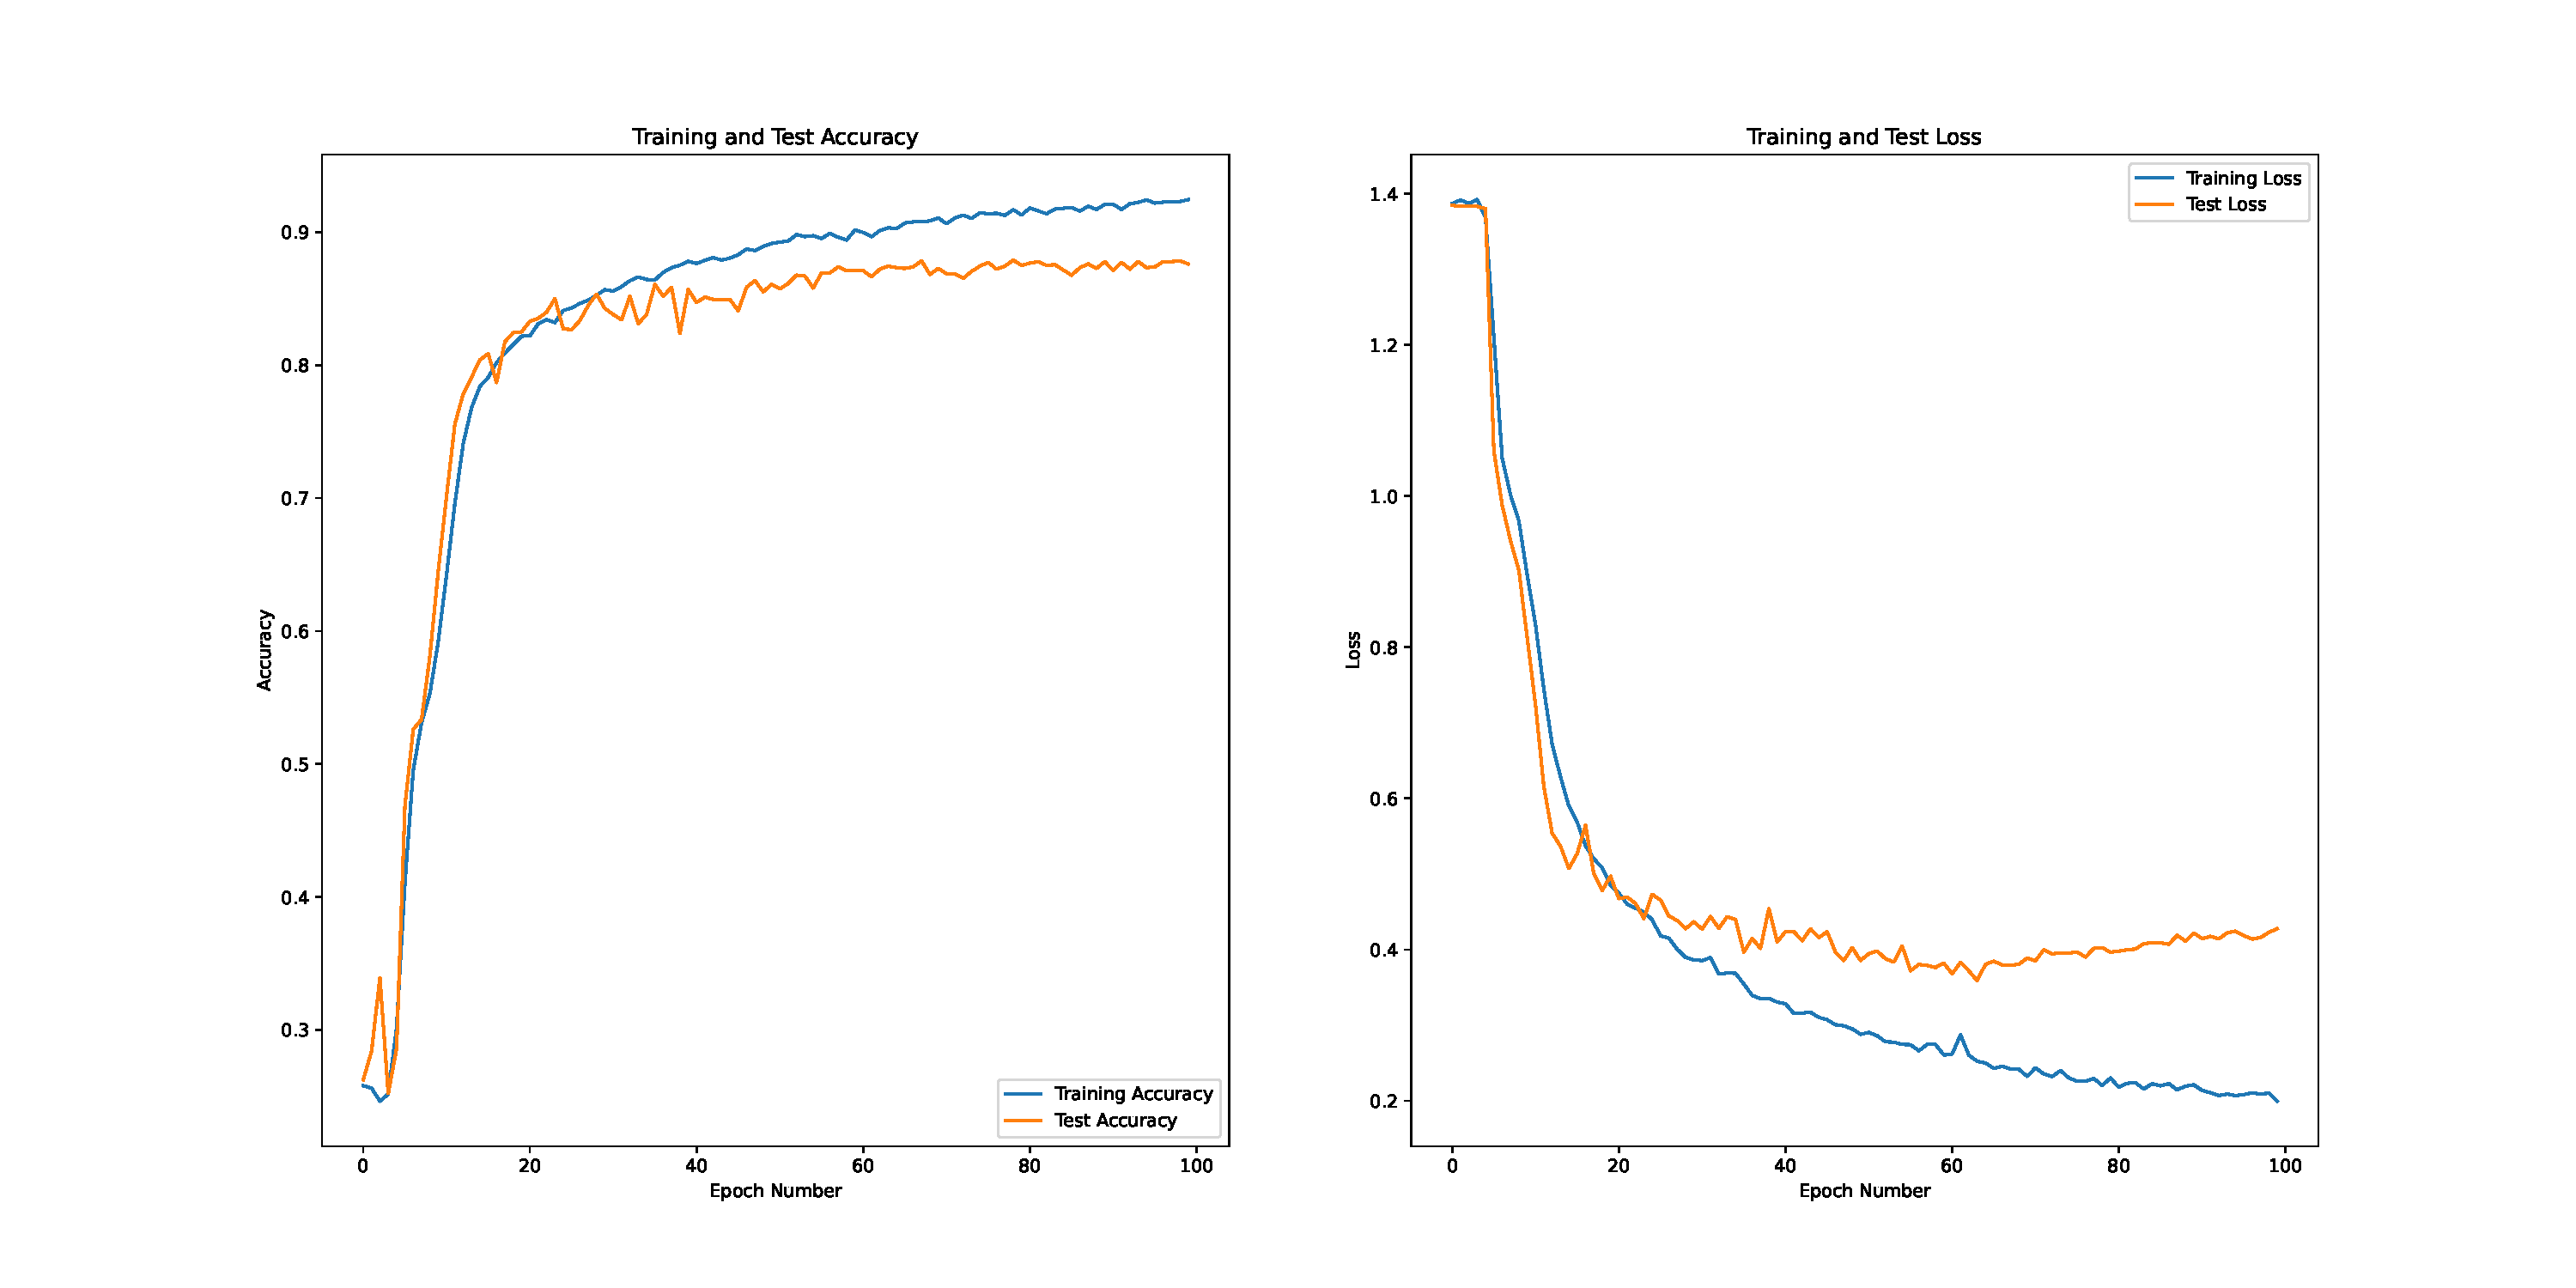
\includegraphics[width=1\textwidth]{metrics/6 metrics.pdf}
\caption[Experiment 6 results]{Experiment 6 results. This shows the impact of a further set of \gls{data_augmentation}s: landmark rotations. The result of this shows decreased performance and a more overfit model.}
\label{fig:6 results}
\end{figure}
\begin{table}
\centering
\begin{tabular}{|c|c|c|c|} 
 \hline
 Experiment &  Testing Accuracy & Testing Loss & \acrshort{wer} \\ [0.2ex] 
 \hline
 6 & \accuracysix & \losssix & \wersix \\ 
 \hline
\end{tabular}
\caption[The testing accuracy, loss and \acrshort{wer} for experiment 6]{The testing accuracy, loss and \acrshort{wer} for experiment 6.}
\label{table: 6 results}
\end{table}
Shown in Figure~\ref{fig:6 results} and Table~\ref{table: 6 results}, the results of this experiment reflected reduced performance, showing that the \gls{data_augmentation} was not beneficial. This may be due to the random rotations not being drastic enough or the amount of \gls{data_augmentation} being too much.\\
Previous to this experiment, each data sample was technically in the dataset twice already: having been augmented once. Random rotations meant that single data samples, although augmented, were presented to the model up to four times. Consequently, \gls{overfitting} could have been due to the structure of the sentences within the data samples, and repeated samples with these structures. Repeated noise might have been causing \gls{overfitting}. Consequently, this extra \gls{data_augmentation} method was not applied to further experiments.
\section{Experiment 7: Transformer Architecture}
\label{sec: Experiment 7}
% Experiment 12a
% Attention/transformer 
\subsection{Model Architecture}
\begin{figure}
\centering
\includegraphics[width=0.9\textwidth]{model architectures/7 architecture.png}
\caption[Experiment 7 architecture]{Experiment 7 architecture. This comprised of an input layer accepting landmark features followed by a series of three encoder blocks. Encoder blocks were made up of multi-head attention blocks and \emph{Add\&Norm} layers. Finally, a feed-forward network was used at the end, before the final hidden representation was fed into a prediction layer.}
\label{fig:7 architecture}
\end{figure}
For this experiment a different model architecture was used, shown in Figure~\ref{fig:7 architecture}. The mechanism of attention, explained in Section~\ref{sec: Attention}, was employed to construct an encoder \gls{transformer} architecture.\\
Landmark features were input and combined with a positional encoding layer\footnote{\url{https://keras.io/api/layers/core_layers/embedding/}}. The output of this was fed into a series of encoder blocks, made up of multi-head attention\footnote{\url{https://keras.io/api/layers/attention_layers/multi_head_attention/}} and \emph{Add\&Norm} layers\footnote{\url{https://keras.io/api/layers/normalization_layers/layer_normalization/}}. The output from this was then fed into a simple feed-forward network and then a dense layer for classification. The purpose of this experiment was to investigate the potential benefits of attention and a \gls{transformer} architecture for lip reading.\\
The same \acrshort{lr} scheduling and batch size was used as experiment 5.5.
\subsection{Results and Evaluation}
\begin{figure}
\centering
\includegraphics[width=1\textwidth]{metrics/7 metrics.pdf}
\caption{Experiment 7 results}
\label{fig:7 results}
\end{figure}
\begin{table}
\centering
\begin{tabular}{|c|c|c|c|} 
 \hline
 Experiment &  Testing Accuracy & Testing Loss & \acrshort{wer} \\ [0.2ex] 
 \hline
 7 & \accuracyseven & \lossseven & \werseven \\ % Original transformer architecture
 \hline
\end{tabular}
\caption{The testing accuracy, loss and \acrshort{wer} for experiment 7.}
\label{table: 7 results}
\end{table}
Shown in Figure~\ref{fig:7 results} and Table~\ref{table: 7 results}, the resulting model performed worse than previous models. \Gls{overfitting} occurred but, as a proof of concept, the \gls{transformer} architecture for lip reading was highly successful. Therefore, further experimentation was carried out to assess this architecture further.
\section{Experiment 8: Image and Landmarks}
\label{sec: Experiment 8}
% Experiment 12c
% Image & landmark data combined
\subsection{Model Architecture}
\begin{figure}
\centering
\includegraphics[width=1\textwidth]{model architectures/8 architecture.png}
\caption[Experiment 8 architecture]{Experiment 8 architecture. This architecture was based on the work of Xue et al.~\cite{lipreading_with_attention}. The model took both visual and landmark features as input to an encoder. The encoder employed self-attention and \emph{Add\&Norm} on either input before using cross-attention between them. The output was then fed into a series of convolutional layers and the prediction layer.}
\label{fig:8 architecture}
\end{figure}
For this experiment, the \gls{transformer} architecture was adapted to improve performance. Inspired by Xue et al.~\cite{lipreading_with_attention}, both visual and landmark features were utilised as inputs to a model, to investigate their potential combined benefit.\\ 
As depicted within Figure~\ref{fig:8 architecture}, visual and landmark features were fed into independent self-attention blocks. These blocks consisted of dot-product self-attention\footnote{\url{https://keras.io/api/layers/attention_layers/attention/}} and \emph{Add\&Norm} layers\footnote{\url{https://keras.io/api/layers/normalization_layers/layer_normalization/}}. The two streams were then fed into similar cross-attention blocks. These blocks instead used the query from one input stream and the key from the alternate stream, hence comparing the two streams and, therefore, formulating cross-attention. The output from this was passed through a further \emph{Add\&Norm} layer before being input into a \acrshort{cnn}. Xue et al. utilised a series of \acrshort{gru} units but our research found that convolutional layers performed better.\\
The same \acrshort{lr} scheduler was used as in experiment 5.5 for better comparison of the new model architecture.
\subsection{Results and Evaluation}
\begin{figure}
\centering
\includegraphics[width=1\textwidth]{metrics/8 metrics.pdf}
\caption{Experiment 8 results}
\label{fig:8 results}
\end{figure}
\begin{table}
\centering
\begin{tabular}{|c|c|c|c|} 
 \hline
 Experiment &  Testing Accuracy & Testing Loss & \acrshort{wer} \\ [0.2ex] 
 \hline
 8 & \accuracyeight & \losseight & \wereight\\
 \hline
\end{tabular}
\caption{The testing accuracy, loss and \acrshort{wer} for experiment 8.}
\label{table: 8 results}
\end{table}
As depicted in Figure~\ref{fig:8 results} and Table~\ref{table: 8 results}, this model architecture produced one of the best performances for lip reading yet. Utilising both landmark and visual features with this \gls{transformer} architecture provides another, different solution for lip reading.\\
The performance of this model was not as good as experiment 5.4 and so further experimentation was carried out.
\section{Experiment 9: CTC Loss}
\label{sec: Experiment 9}
% Experiment 13a,b,c
% CTC loss: 
% Same architecture but different loss measure
\subsection{Model Architecture}
For this experiment, the same model architecture was used as experiment 8, however, the classes and loss metric were changed.\\
Outlined in Section~\ref{sec: CTC Loss}, \acrshort{ctc} loss is a useful loss metric capable of drawing connections between two sequences when this alignment is unknown~\cite{exploration-of-CTC-acoustic-models}. This fits the task of aligning a set of letters, \gls{phoneme}s or \gls{viseme}s to a sequence of video frames.\\
This experiment focused on experimenting with \acrshort{ctc} loss to make three different models capable of predicting the letter, \gls{phoneme} and \gls{viseme} uttered in each frame.\\
Because a different loss metric has been used to train these models, they cannot be directly compared to the previous experiments. Different loss metrics mean that we must independently inspect these models and their performance with lip reading.\\
Different class labels were used for these experiments, changing from \gls{single-label} to \gls{multi-label}. For experiment 9.1 these were the letters for the word uttered, experiment 9.2 used the \gls{phoneme}s and experiment 9.3 used the \gls{viseme}s. This transformed the classes from 1D \gls{one_hot_encoding}s to instead 1D vectors of class numbers.\\
The same \acrshort{lr} scheduling method was used as in experiment 5.5.
\subsection{Results and Evaluation}
\begin{figure}
\centering
    \subfloat[\centering Letter based model]{\includegraphics[width=0.5\textwidth]{metrics/9.1 metrics.pdf}}
    \subfloat[\centering \Gls{phoneme} based model]{\includegraphics[width=0.5\textwidth]{metrics/9.2 metrics.pdf}}\\
    \subfloat[\centering\Gls{viseme} based model]{\includegraphics[width=0.5\textwidth]{metrics/9.3 metrics.pdf}}
\caption[Experiment 9 results]{Experiment 9 results. Three different sub-experiments were conducted, using \acrshort{ctc} loss, to compare using the letters, \gls{phoneme}s and \gls{viseme}s as classes for lip reading.}
\label{fig:9 results}
\end{figure}
\begin{table}
\centering
\begin{tabular}{|c|c|c|c|c|} 
 \hline
 Experiment & Class Types &  Testing Accuracy & Testing Loss & \acrshort{wer} \\ [0.2ex] 
 \hline
 9.1 & Letter & \accuracynineone & \lossnineone & \wernineone \\
 9.2 & \Gls{phoneme} & \accuracyninetwo & \lossninetwo & \werninetwo \\
 9.3 &\Gls{viseme} & \accuracyninethree & \lossninethree & \werninethree \\
 \hline
\end{tabular}
\caption[The testing accuracy, loss and \acrshort{wer} for experiment 9]{The testing accuracy, loss and \acrshort{wer} for experiment 9. Three different sub-experiments were conducted, using \acrshort{ctc} loss, to compare using the letters, \gls{phoneme}s and \gls{viseme}s as classes for lip reading.}
\label{table: 9 results}
\end{table}
The findings of this experiment, presented within Table~\ref{table: 9 results} and Figure~\ref{fig:9 results}, are incredibly interesting. As suspected, the best class for lip reading was indeed \gls{viseme}-based, followed by \gls{phoneme}-based and finally letter-based. This is intuitive as many letters in the English language are not pronounced or are pronounced differently depending on the context. For example, the ``h" in ``her" and ``there" are very different.\\
\Gls{phoneme}-based lip reading presented the worst accuracy but better loss and \acrshort{wer} compared with the other methods. A potential reason for this may be some \gls{phoneme}s not being visually represented. Especially in the English lexicon, many sounds are spoken quickly, skipped or pronounced without changes to the facial position. Consequently, the model may struggle to distinguish some words based on their \gls{phoneme}s.\\
The finding that \gls{viseme}-based learning is useful for lip reading is incredibly important and shows the impact of focusing on visual aspects of speech. Furthermore, this proof of concept shows that many visual-only lip reading systems could be improved and made more generic and able to process far more words by looking at their sub-words, particularly their \gls{viseme}s.\\ %Chapter 4
%   Results: ~ 27.5%: 4125 words
        % Current: 2767 words
\chapter{Conclusion}
\label{cha:conclusion}
\section{Summary of Achievements}
\begin{table}[h!]
\centering
\begin{tabular}{|c|c|c|c|c|} 
 \hline
 Experiment & Summary &  Val Accuracy & Val Loss & \acrshort{wer} \\ [0.2ex] 
 \hline
 4.2 & Visual-based & \accuracyfourtwo & \lossfourtwo & \werfourtwo \\
 5.4 & Landmark-based \acrshort{bilstm} & \accuracyfivefour & \lossfivefour & \werfivefour \\
 8 & Landmark, Visual \Gls{transformer} & \accuracyeight & \losseight & \wereight \\
 \hline
  9.1 & Letter-based with \acrshort{ctc} loss & \accuracynineone & \lossnineone & \wernineone \\
 9.2 & Phoneme-based with \acrshort{ctc} loss & \accuracyninetwo & \lossninetwo & \werninetwo \\
 9.3 & Viseme-based with \acrshort{ctc} loss & \accuracyninethree & \lossninethree & \werninethree \\
 \hline
\end{tabular}
\caption[The final models presented for lip reading]{The final models presented for lip reading. This shows the testing accuracy, loss and \acrshort{wer} achieved for the best lip reading models trained within this research. There is slight variation within the design, architecture and training of these models, outlined within the relevant sections above.}
\label{table: final models}
\end{table}
In this research, we aimed to compare different methods of using \acrlong{ml} and \acrlong{cv} for visual-only lip reading.\\
We started by developing a data generation pipeline to preprocess data from the BBC into a format that could be trained upon. The \gls{lrw} dataset was selected due to its reliability and because it suited the independent word recognition task studied here.\\
Various architectures were trained, compared, and modified to create the best lip reading solution. First, simple architectures such as \acrfull{cnn} and \acrfull{bilstm} networks were investigated, but later more complex \gls{transformer} architectures were used to great success. The \acrfull{lr} was significantly varied and exploited to create the best possible models. From this research, it was discovered that \gls{transformer} architectures and \acrshort{bilstm} networks performed the best for lip reading. It was also found that a combination of landmark and visual inputs can improve lip reading performance.\\
Finally, \acrfull{ctc} loss was used to train lip reading \acrshort{ann}s capable of processing each independent frame, distinguishing each sub-word and predicting the letter, \gls{phoneme} or \gls{viseme} uttered. These models were compared to find the best solution for frame-to-frame lip reading which was, as hypothesised, \gls{viseme}-based prediction.\\
Overall, seventeen experiments were conducted. A summary of the best models developed for lip reading is displayed in Table~\ref{table: final models}, displaying up to 97\% accuracy, less than 10\% loss and a \acrfull{wer} of just 13.7\%. A summary of all of the results of these experiments is shown in Table~\ref{table: all models}.\\
Overall, all of the objectives established in Section~\ref{sec:Aims and Objectives} were achieved. An efficient, configurable and automatic data generation pipeline was developed, making it easier to extend this work in the future. Various \acrshort{ann} architectures were designed, trained and objectively compared to find the best solution for lip reading. A \acrfull{gui} was also developed to showcase the different models and alter the processing of their outputs. Additionally, the \acrshort{gui}'s extensional aim was achieved by incorporating model fine-tuning, which improved lip reading performance for specific users.
\section{Critical Reflection}
As with any project, it is crucial to reflect upon its inherent strengths and weaknesses. This reflection aims to highlight potential areas of improvement whilst implementing lip reading using \acrfull{ml}.\\
One major limitation of this work was the size of the data involved. Much of the training and experimentation was limited to a small subset of words. This decision was taken to shorten the potential long training times, reduce the required data storage and avoid some difficult issues such as with high-dimensional classification. The small word set allowed further focus on the task at hand. Whilst the findings from this experiment were conducted with rigorous adherence to the scientific method, and with a large amount of data, further words could have been incorporated to offer better reliability, additional comparison of model performance and create a more general model suitable for wider application. Future improvements could extend the vocabulary, trying a larger set of words and potentially comparing sub-word and word-level classification. This work could take the achievements found with the \gls{transformer} architecture and \acrshort{ctc} loss, extending them to a wider dataset.\\
Another limitation of this work was the intrinsic nature of model evaluation. Testing and evaluation were primarily completed using data from the \gls{lrw} dataset, with some testing via the \acrshort{gui}. Extrinsic evaluation, on completely unseen and different data, would give a better understanding of the generalisability, application and true performance of the lip reading models. All data within the \gls{lrw} dataset is similar, making the analysis less reliable. Future work could validate these models against external data from a setting that is completely unseen. This would give additional information as to the usefulness of models and provide further insight as to methods for further improving model performance.\\
Finally, due to timing constraints, and it not being the true focus of the project, the \acrshort{gui} was not as usable or aesthetic as it could have been. The aims of this project were primarily around lip reading research and model comparison, rather than developing an efficient application. Further time could extend this \acrshort{gui} into a more usable application, with user evaluation even being carried out to maximise the user experience of a formal lip reading application.
\section{Future Work}
The research conducted in this study offers numerous avenues for potential applications. This section will explain some potential extensions or uses of the work.\\
Firstly, and the most obvious, would be to extend the experiments conducted within this research. Models could be trained to recognise wider word sets, different model architectures could be trialled or further parameter settings could be assessed. Continually, new architectures are found that perform better in specific situations. Creating different model architectures, training them for lip reading and comparing their performance would help to extend the research further. The experiments above have various parameters that could be investigated in more depth.\\
Some suggestions for variations on experiments include:
\begin{itemize}
    \item During data preprocessing, utilise a larger set of MediaPipe landmarks than the forty selected for this research. An entirely different facial landmark system could be investigated, such as the solution provided by DLib
    \item During data preprocessing, crop a larger region of the mouth or face
    \item Compare different visual feature extractors and their performance during training
    \item Expand the word set for training
    \item Expand testing to an unseen task or different dataset
    \item Train a specific visual feature extractor for human faces, rather than employing a pretrained extractor
\end{itemize}
Next, whilst this approach was research-centered, further work could use the findings here to develop an application built around lip reading. Hardware could specifically be made to help people with hearing loss on the go. For example, a pair of glasses could be made to employ lip reading in real-time. Uni-directional microphones could be used to focus on a single person and collect audio to be paired with visual features. This technology could improve closed caption generation, could generate audio in a visual-only medium or improve security. Many security cameras are outdated, giving no audio, so such a model could help law enforcement to listen to criminal activity from such cameras.\\
In summary, there are various ways this research could be extended. Lip reading is crucial to everyday communication and \acrlong{ml} presents a new way forwards that could greatly improve audio processing, give insight into teaching lip reading and help people with \acrfull{dhl}.             %Chapter 5
%   Conclusion: ~ 5%: 750 words
        % Current: 1038 words

  \bibliography{refs}    % this causes the references to be listed

\bibliographystyle{abbrv}
%% the bibliography style determines the format  in which both citations and references are printed,
%% other possible values are plain and abbrv
%%
%% If you want more control of the format of your citations you might want to take a look at
%% natbib.sty, which should be part of any standard LaTeX installation
%%
%% University regulations simply require that your citation style be consistent, so see what style
%% your supervisor recommends.

% Appendices start here

\appendix
\chapter{Model Metric Summary}
\label{cha: Appendix}
% \section{Model Metric Summary}
\begin{table}[h!]
\centering
\begin{tabular}{|c|c|c|c|} 
 \hline
 Experiment &  Validation Accuracy & Validation Loss & \acrshort{wer} \\ [0.2ex] 
 \hline
 1 & \accuracyone & \lossone & \werone \\
 2 & \accuracytwo & \losstwo & \wertwo \\ 
 3 & \accuracythree & \lossthree & \werthree \\
 4.1 & \accuracyfourone & \lossfourone & \werfourone \\
 4.2 & \accuracyfourtwo & \lossfourtwo & \werfourtwo \\
 4.3 & \accuracyfourthree & \lossfourthree & \werfourthree \\
 5.1 & \accuracyfiveone & \lossfiveone & \werfiveone \\
 5.2 & \accuracyfivetwo & \lossfivetwo & \werfivetwo \\ 
 5.3 & \accuracyfivethree & \lossfivethree & \werfivethree \\
 5.4 & \accuracyfivefour & \lossfivefour & \werfivefour \\
 5.5 & \accuracyfivefive & \lossfivefive & \werfivefive \\
 6 & \accuracysix & \losssix & \wersix \\
 7 & \accuracyseven & \lossseven & \werseven \\
 8 & \accuracyeight & \losseight & \wereight \\
 \hline
 9.1 & \accuracynineone & \lossnineone & \wernineone \\
 9.2 & \accuracyninetwo & \lossninetwo & \werninetwo \\
 9.3 & \accuracyninethree & \lossninethree & \werninethree \\
 \hline
\end{tabular}
\caption[Comparative metrics for all models trained]{Comparative metrics for all models trained. This shows the validation accuracy, loss and \acrshort{wer} (where applicable) for all different trained models. Note that lines are used between models that cannot be compared either due to a different training data, loss metrics or otherwise.}
\label{table: all models}
\end{table}

\end{document}
